\documentclass{atlasnote} 
\graphicspath{{figures/20140510_Prelim/}}
\usepackage{atlasphysics}
\usepackage{subfigure}
\usepackage{mathrsfs}
\usepackage{xspace}            % for correct spacing after commands
\usepackage{bm}                % bold math
\usepackage[pdfauthor={ATLAS Collaboration}, pdftitle={Tagging and suppression of pileup jets}, bookmarks=true, breaklinks = true, colorlinks=true,
            linkcolor=blue, citecolor=magenta]{hyperref} % bookmarks  


%% --------  Style ----------------
\makeatletter 
% -- Make maths in section titles go automatically bold --
\DeclareRobustCommand*{\bfseries}{%
  \not@math@alphabet\bfseries\mathbf
  \fontseries\bfdefault\selectfont
  \boldmath
}

% -- make subsubsection font size to be large   --
\renewcommand\subsubsection{\@startsection{subsubsection}{3}{\z@}%
                                     {-3.25ex\@plus -1ex \@minus -.2ex}%
                                     {1.5ex \@plus .2ex}%
                                     {\normalfont\large\bfseries}}
% -- make paragraph text to start in a new line --
\renewcommand\paragraph{\@startsection{paragraph}{4}{\z@}%
                                    {-3.25ex \@plus -1ex \@minus -.2ex}%
                                    {1.2ex \@plus .2ex}%
                                    {\normalfont\normalsize\bfseries}}

\makeatother 
%-----------------------------------

%%%%%%%%%%%%%%%%%%%%%%%%%%%%%%%%%%%%
%           Title page             % 
%%%%%%%%%%%%%%%%%%%%%%%%%%%%%%%%%%%%

\skipbeforetitle{100pt}

% Title
\title{Tagging and suppression of pileup jets with the ATLAS detector}

% if multiple authors/affiliations are needed, use the authblk package
\usepackage{authblk}
\renewcommand\Authands{, } % avoid ``. and'' for last author
\renewcommand\Affilfont{\itshape\small} % affiliation formatting

\author{The ATLAS Collaboration}

\atlasnote{ATLAS-CONF-2014-018}

% Date: if not given, uses current date
%\date{\today}

% Draft version: if given, adds draft version on front page, a
% 'DRAFT' box on top of each other page, and line numbers to easy
% commenting. Comment or remove in final version.
% \draftversion{8.0}

% Journal: adds a 
%\journal{Phys. Lett. B} 

% Abstract
\abstracttext{
The suppression of pileup jets has been a crucial component of many 
physics analyses using 2012 LHC proton-proton collisions. In ATLAS, 
tracking information has been used to calculate a variable called the 
jet-vertex-fraction, which is the fraction of the total momentum of 
tracks in the jet which is associated with the primary vertex. Imposing a 
lower limit on this variable rejects the majority of pileup jets, but leads to 
hard-scatter jet efficiencies that depend on the number of 
reconstructed primary vertices in the event (\NPV). In this note, 
new track-based variables to suppress pileup jets are developed in 
such a way that the resulting hard-scatter jet efficiency is stable as 
a function of \NPV. A multivariate combination of two such variables 
called the jet-vertex-tagger (\JVT) is constructed. 
The modeling of \JVT is tested in $\Zboson(\to\mu\mu)$+jets as well as in 
semileptonic \ttbar events. 
The efficiencies of different \JVT criteria are measured in data and compared to simulation.
In addition, it is 
shown that jet-vertex association can be applied to large-$R$ jets, 
providing a track-based grooming technique that is as powerful as 
calorimeter-based trimming but based on complementary tracking 
information. Finally, the performance of track-based grooming is 
compared with the recently proposed jet cleansing algorithm. 
\newline\newline
\textit{
Revised figure 18 with respect to the version of May 12, 2014
}
}

%%%%%%%%%%%%%%%%%%%%%%%%%%%%%%%%%%%%
%            Defines               %
%%%%%%%%%%%%%%%%%%%%%%%%%%%%%%%%%%%%

% % counters
\newcounter{fixme}
\newcommand{\fixme}[1]{{\it{\textbf{Fixme~\arabic{fixme}~(#1)}}}\addtocounter{fixme}{1}}
% \newcounter{idea}
% \newcommand{\idea}[1]{{\it{\textbf{\textcolor{Cerulean}{Idea~\Roman{idea}~(#1)}}}\\}\addtocounter{idea}{1}}
% 
% i.e. and so on
\newcommand {\ie}{\mbox{i.e.}\xspace}     %i.e.
\newcommand {\vs}{\mbox{vs.}\xspace}     %i.e.
\newcommand {\hc}{\mbox{h.c.}\xspace}     %i.e.
\newcommand {\eg}{\mbox{e.g.}\xspace}     %e.g.

% misc
\newcommand{\bfit}[1]{\textit{\textbf{#1}}}
\newcommand{\Eqref}[1]{Eqn.~\eqref{#1}}
\newcommand{\Figref}[1]{Fig.~\ref{#1}}
\newcommand{\beq}{\begin{equation}}
\newcommand{\eeq}{\end{equation}}
\newcommand{\sign}{\ensuremath{\text{sign}\xspace}}

% particles 
\renewcommand{\Zboson}{\ensuremath{Z}\xspace}
\newcommand{\Higgs}{\ensuremath{H}\xspace}
\renewcommand{\Wboson}{\ensuremath{W}\xspace}
\newcommand{\proton}{\ensuremath{{\mathrm{p}}\xspace}}
\newcommand{\pq}{\ensuremath{{\mathrm{q}}\xspace}}
\newcommand{\pb}{\ensuremath{{\mathrm{b}}\xspace}}
\newcommand{\pbbar}{\ensuremath{{\mathrm{\bar{b}}}\xspace}}
\renewcommand{\ttbar}{\ensuremath{{\mathrm{t\bar{t}}}}\xspace}

%units
\newcommand{\unit}[1]{\ensuremath{\,\text{#1}}\xspace}
\newcommand{\Unit}[1]{\ensuremath{\,\rm{$#1$}}\xspace}
\newcommand{\Lumino}{20.3\unit{\ifb}}
\renewcommand{\GeV}{\ensuremath{\,\text{Ge\hspace{-.08em}V}}\xspace}
\renewcommand{\TeV}{\ensuremath{\,\text{Te\hspace{-.08em}V}}\xspace}

% subequations
\newcommand{\eqn}[2]{\begin{subequations}\label{#1} #2 \end{subequations}}

% kinematic variables
\newcommand{\MTtwo}{\ensuremath{M_\mathrm{T2}}\xspace}
\newcommand{\JVF}{\ensuremath{{\rm JVF}}\xspace}
\newcommand{\JVT}{\ensuremath{{\rm JVT}}\xspace}
\newcommand{\cJVF}{\ensuremath{{\rm corrJVF}}\xspace}
\newcommand{\RpT}{\ensuremath{R_\mathrm{pT}}\xspace}
\newcommand{\PURpT}{\ensuremath{R_\mathrm{pT}^{\mathrm{PU}}}\xspace}
\newcommand{\NPV}{\ensuremath{N_\mathrm{Vtx}}\xspace}
\newcommand{\NPVtruth}{\ensuremath{N_\mathrm{Vtx}^{\rm truth}}\xspace}
\renewcommand{\pT}{\ensuremath{p_{\mathrm{T}}}\xspace}
\newcommand{\nPUtrk}{\ensuremath{n_\mathrm{trk}^\mathrm{PU}}\xspace}
 
% generators
\newcommand{\HERWIG}         {\mbox{\small\textsc{HERWIG}}}
\newcommand{\HDECAY}         {\mbox{\small\textsc{HDECAY}}}
\newcommand{\ggWWp}         {\mbox{\small\textsc{GG2WW}}}
\newcommand{\DIPHOX}         {\mbox{\small\textsc{DIPHOX}}}
\newcommand{\AR}         {\mbox{\small\textsc{ARIADNE}}}
\newcommand{\ALPGEN}         {\mbox{\small\textsc{Alpgen}}}
\newcommand{\PY}         {\mbox{\small\textsc{PYTHIA}}}
\newcommand{\JSv}        {\mbox{\small\textsc{JETSET\ 7.405}}}
\newcommand{\HWo}        {\mbox{\small\textsc{HERWIG\ 5.8}}}
\newcommand{\HWn}        {\mbox{\small\textsc{HERWIG\ 5.9}}}
\newcommand{\ARv}        {\mbox{\small\textsc{ARIADNE\ 4.05}}}
\newcommand{\PYv}        {\mbox{\small\textsc{PYTHIA\ 5.7}}}
\newcommand{\MADGRAPH}   {\textsc{MadGraph}\xspace}
\newcommand{\Sherpa}   {\textsc{Sherpa}\xspace}
\newcommand{\MADGRAPHv}   {\textsc{MadGraph}\ 5v1.1\xspace}
\newcommand{\BRIDGE}   {\textsc{Bridge}\xspace}
\newcommand{\PYTHIA}    {\textsc{Pythia}\xspace}
\newcommand{\PYTHIAeight}    {\textsc{Pythia8}\xspace}
\newcommand{\DELPHES}   {\textsc{Delphes}\xspace}
\newcommand{\GEANTfour} {{\textsc{geant4}}\xspace}
\newcommand{\JetPhox}    {\textsc{JetPhox\ 1.3.0}\xspace}
\newcommand{\Powheg}    {\textsc{PowHeg}\xspace}
\newcommand{\Fastjet}   {\textsc{Fastjet\ 2.4.3}\xspace}

% other programs
\newcommand{\SOFTSUSY}         {\mbox{\small\textsc{SoftSusy}}\xspace}
\newcommand{\PROSPINO}         {\mbox{\small\textsc{Prospino}}\xspace}

\newcommand{\ATLAS}{{\textsc ATLAS}\xspace}



%%%%%%%%%%%%%%%%%%%%%%%%%%%%%%%%%%%%
%            Content               % 
%%%%%%%%%%%%%%%%%%%%%%%%%%%%%%%%%%%%

\begin{document}

% ------------- Introduction -----------------------
\section{Introduction}
At the Large Hadron Collider (LHC) the collisions of proton (p) bunches result not only in hard-scatter (signal) pp interactions, but also
in additional collisions accompanying the signal. Such additional low transverse momentum pp collisions are referred 
to as {\it pileup} interactions. We differentiate between {\it in-time} and {\it out-of-time} pileup. While in-time 
pileup arises from additional pp interactions in the current bunch-crossing, out-of-time pileup refers to energy deposits in the ATLAS 
calorimeter~\cite{ATLAS:JINST} from previous and following bunch crossings relative to the triggered event.
For this note, in-time and out-of-time pileup will be referred to collectively as pileup.

The additional transverse energy flow from pileup interactions 
is typically subtracted on average from the signal interaction of interest. 
Local fluctuations in the pileup activity, however, 
may result in spurious pileup jets.
In Ref.~\cite{ATLASConfNote:PUcorrection} it was shown that pileup jets can be 
effectively removed by a minimal jet-vertex-fraction (\JVF) requirement. 
The \JVF variable is defined as the scalar transverse momentum (\pT) 
sum of the tracks that are associated with the jet and originate from the hard-scatter vertex divided by the scalar \pT sum of all associated tracks:
%---------
\begin{equation}
\JVF = \frac{\sum_k{\pT^{{\rm trk}_k}({\rm PV}_0)}}{\sum_l \pT^{{\rm trk}_l}({\rm PV}_0) + \sum_{n\geq1}\sum_l \pT^{{\rm trk}_l}({\rm PV}_n)} 
\label{eq:JVF}
\end{equation}
%---------
Here, $\rm PV_0$ is the hard-scatter vertex (see section~\ref{sec:OS}) and $\rm PV_j$, $j\geq1$ corresponds to primary vertices due to pileup interactions in the same bunch crossing. 
\JVF is bound between 0 and 1, but a value of $-1$ is assigned to jets with no associated tracks. 
It measures the fractional \pT from tracks associated with the hard-scatter vertex. 
As the denominator of \JVF increases with the number of reconstructed primary vertices in the event 
(\NPV\footnote{%
The vertex reconstruction efficiency depends on the average number of interactions per bunch crossing $\mu$ and ranges between $80\%$ 
and $50\%$ for $\mu = 0$ to $\mu = 40$~\cite{ATLAS-CONF-2012-042}.}), due to an increase in the number of pileup tracks associated with the jet, 
the mean \JVF for signal jets is shifted to smaller values, as shown in \Figref{fig:JVFdist_NPVdependence}.
The explicit pileup dependence of \JVF results in an \NPV dependent jet efficiency when a minimal \JVF criterion is 
imposed to reject pileup jets. This effect is illustrated in Figure~\ref{fig:JVF_NPVdependence} for jets in three different \pT bins requiring $\JVF > 0.5$. 
%------------------------
\begin{figure}[!htbp]
  \centering
  \subfigure[]{
      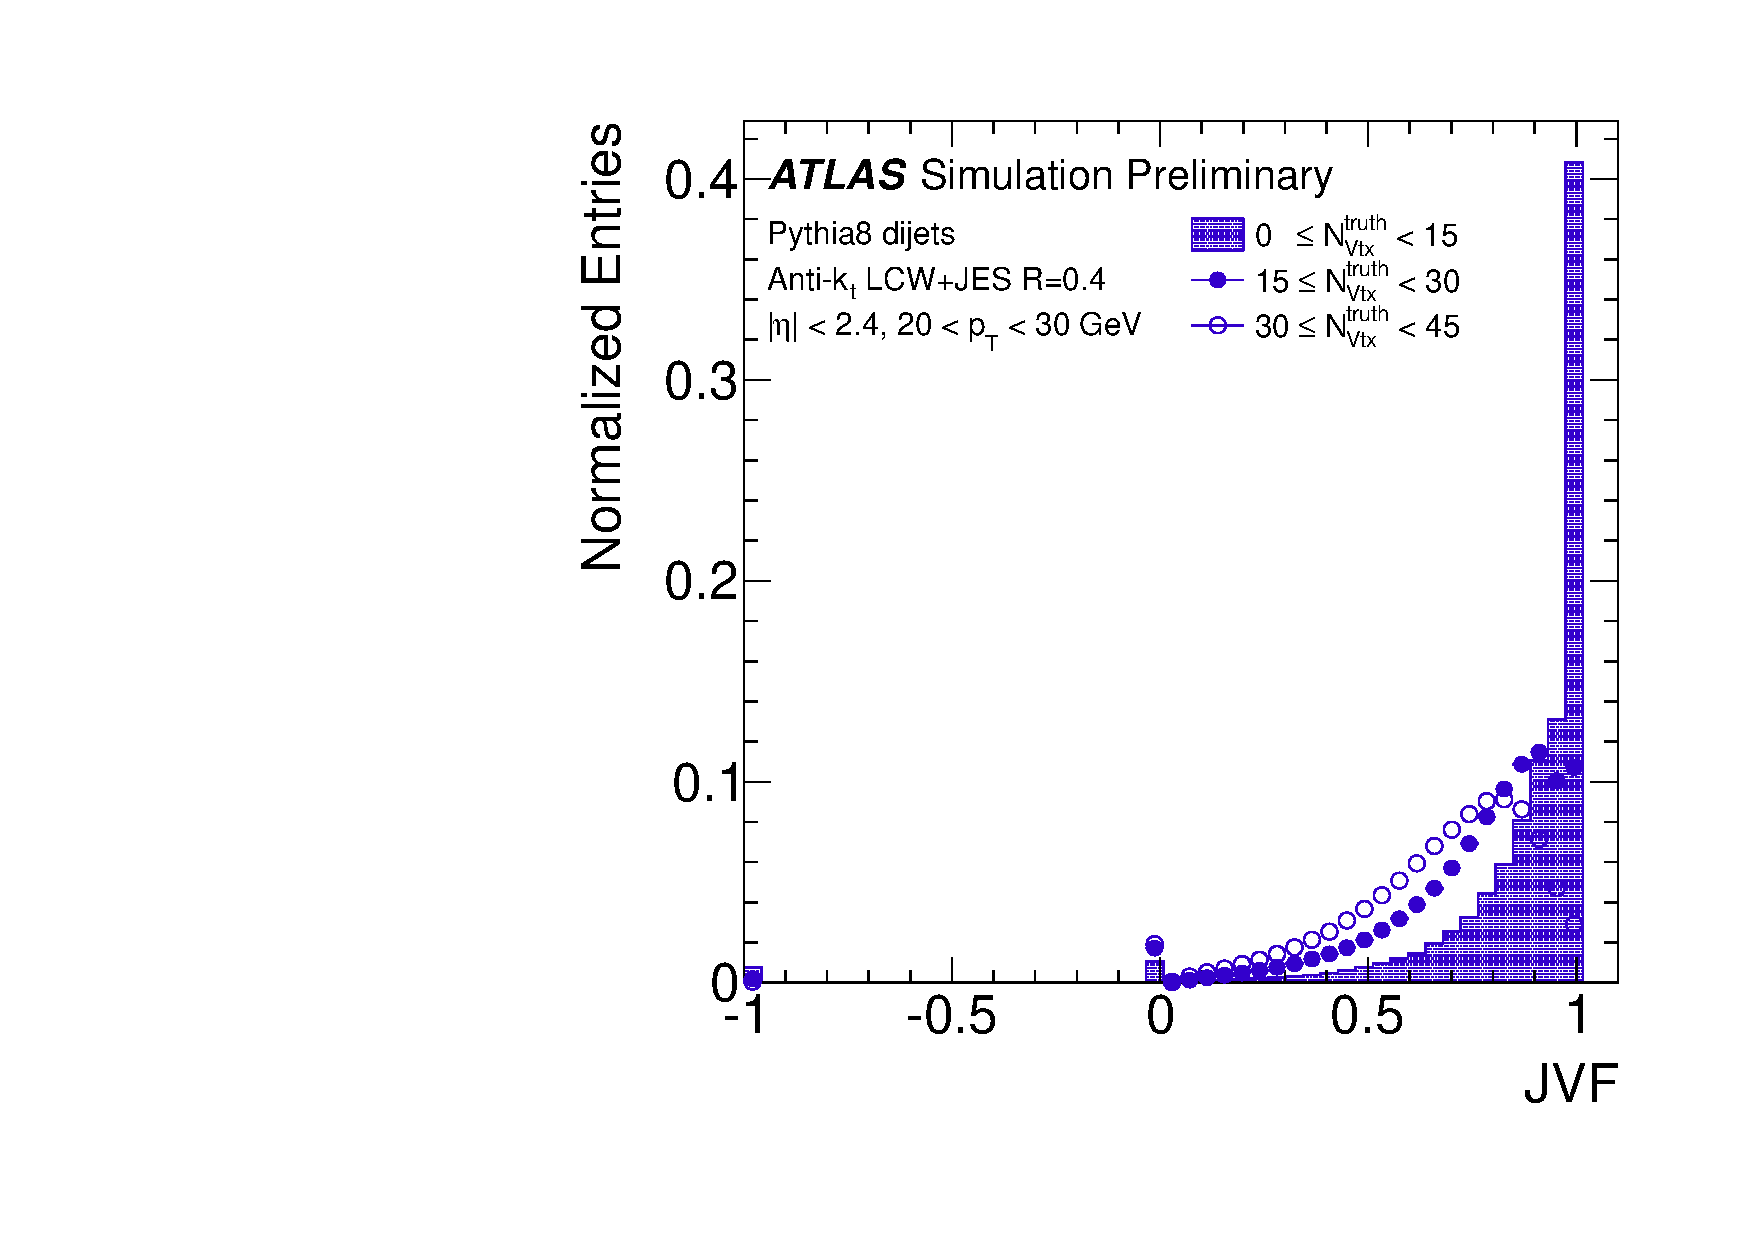
\includegraphics[width= 0.46\textwidth]{JVFDist_HS_differentNPVtruthBins}
    \label{fig:JVFdist_NPVdependence}
  }
  \subfigure[]{
    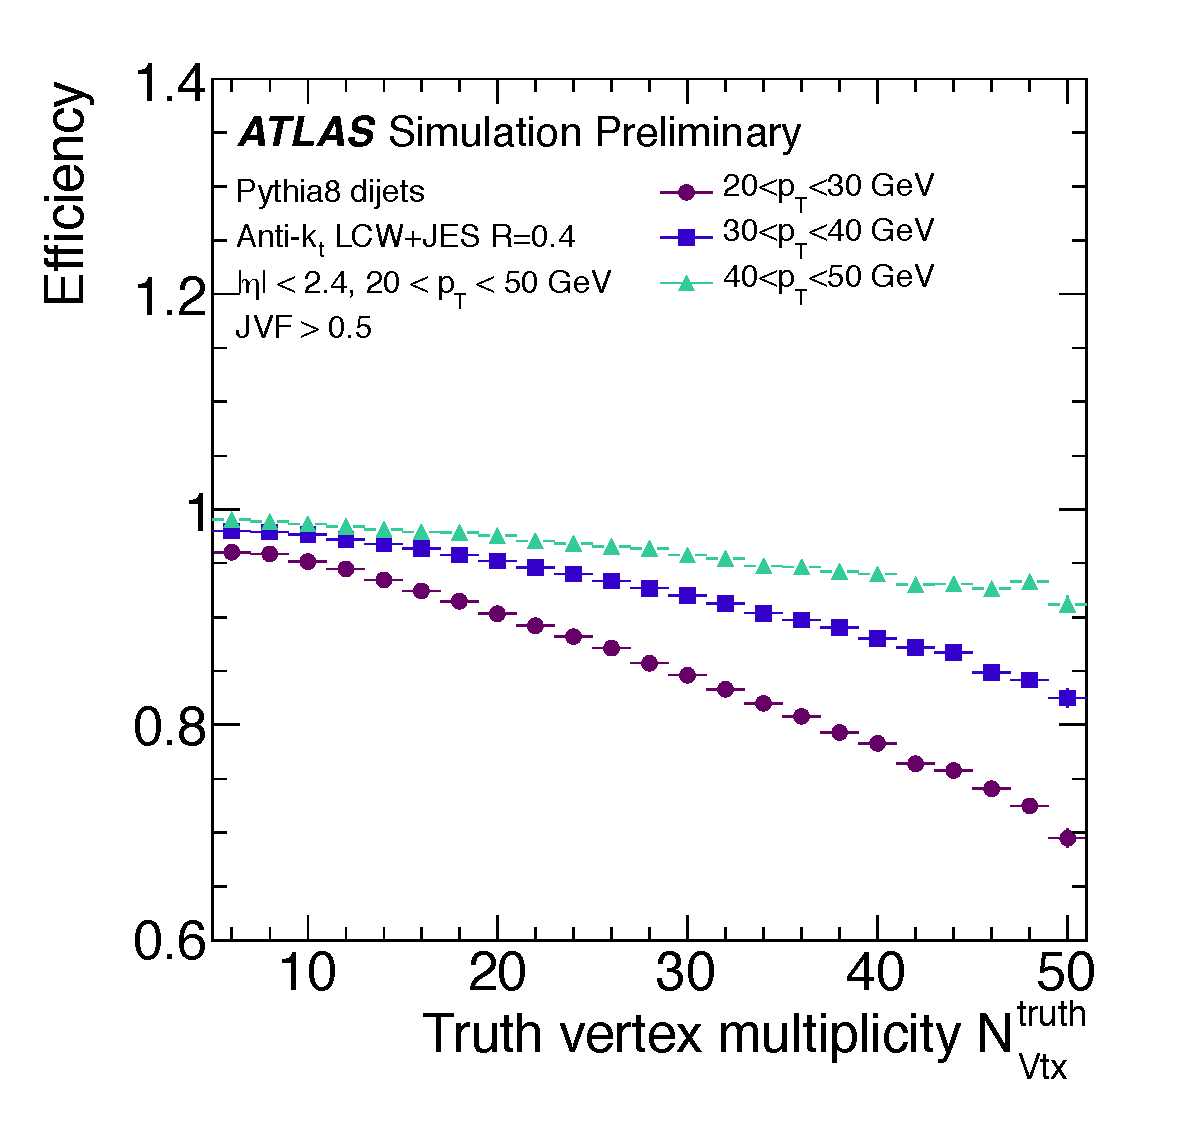
\includegraphics[width= 0.46\textwidth]{JVF_HSeff_NPVTruthDependence}
    \label{fig:JVF_NPVdependence}
  }
  \caption{(a) The JVF distribution for hard-scatter jets (see Section~\ref{sec:OS}) in simulated dijet events for different bins in truth vertex 
  multiplicity \NPVtruth.
  (b) The efficiency of a $\JVF>0.5$ requirement for hard-scatter jets as a function of \NPVtruth, for three different jet \pT bins. 
  \label{fig:JVF_NPVdep}
  }
\end{figure}
%------------------------

In this note, new track-based variables are developed to suppress pileup jets in such
a way that the resulting hard-scatter jet efficiency is stable as a function of \NPV. 
The note is organized as follows. In Section~\ref{sec:selection} a brief description of the ATLAS experiment is presented and the object reconstruction and 
event selection is discussed. Two new track-based variables are introduced in Section~\ref{sec:newvars}, and in Section~\ref{sec:JVT} a multivariate combination 
of these two variables, called the {\it jet-vertex-tagger}, is derived and its performance is characterized. The modeling of the jet-vertex-tagger is 
validated with data in Section~\ref{sec:JVTvalidation}. In Section~\ref{sec:JVTapplication} the application of the jet-vertex-tagger is illustrated in a study of the 
jet multiplicity in $\Zboson(\to\mu\mu)$+jets events as well as for a jet-veto efficiency study in simulated $\Higgs\to\Zboson\Zboson$ events, where the Higgs boson \Higgs is produced via 
vector-boson fusion $( \pq \pq^{\prime} \to \pq \pq^{\prime} \Higgs)$. Section~\ref{sec:grooming} contains a discussion of a novel track-based grooming technique for large-$R$ jets, where jet-vertex association is used
to mitigate pileup effects. Finally, Section~\ref{sec:concl} contains the conclusions. 


\section{Object definition and event selection}
\label{sec:selection}

\subsection{The \ATLAS detector}
The results presented in this paper are based on an integrated luminosity of \Lumino of \proton\proton~collisions recorded with the \ATLAS detector at a center-of-mass energy of 8\TeV during the 2012 data taking. 
\ATLAS is a cylindrical multi-purpose particle detector hermetic in azimuth for a 
pseudorapidity%
\footnote{
\ATLAS uses a right-handed coordinate system with its origin at the nominal interaction point (IP) 
in the centre of the detector and the $z$-axis along the beam pipe. The $x$-axis points from the IP to the centre of the LHC ring, 
and the $y$-axis points upward. Cylindrical 
coordinates $(r, \phi)$ are used in the transverse plane, $\phi$ being the azimuthal angle around the beam pipe. 
The pseudorapidity is defined in terms of the polar angle $\theta$ as $\eta = - \ln \tan(\theta/2)$.
}
%
range of $|\eta|<4.9$. 
It comprises an inner tracking detector, electromagnetic and hadronic sampling calorimeters, and an air-toriod muon system. 
The inner detector, which includes the silicon pixel detector, a silicon microstrip detector and a transition radiation tracker, covers a pseudorapidity range 
$|\eta|<2.5$ and is immersed in a 2\unit{T} axial magnetic field produced by a 
superconducting solenoid. Surrounding the solenoid there are finely-segmented liquid argon and iron-scintillator calorimeters providing precise energy measurements. 
Outside the calorimetry there is a muon spectrometer immersed in a magnetic field provided by three large toroid magnets. 
A multi-level trigger system of dedicated hardware and software filters is used to select \proton\proton~collisions. 
A detailed description of the \ATLAS detector can be found elsewhere~\cite{ATLAS:JINST}.

\subsection{Object reconstruction}
\label{sec:OS}
The reconstruction and definition of physics objects used in this analysis is based on Ref.~\cite{ATLASConfNote:PUcorrection}, 
where more details can be found. 

\paragraph{Vertices and tracks}
The event hard-scatter primary vertex is defined as the 
one reconstructed vertex with the largest $\sum p_{T}^2$ of constituent tracks.
Tracks are selected with $\pT> 0.5\GeV$ and are further required to pass quality criteria 
designed to reject poorly measured and fake tracks. 
A careful association of tracks to vertices is crucial to optimize the separation between pileup and hard-scatter jets. We use the following two-step procedure. 
First, tracks are assigned to vertices based on the track-to-vertex association resulting from the vertex reconstruction~\cite{ATLAS-CONF-2012-042}.
Secondly, tracks that have a $|z_0|<3\unit{mm}$ with respect to the hard-scatter primary vertex and are not associated with any vertex after the first step are 
then assigned to the hard-scatter primary vertex. This additional step is important for jets that are initiated by heavy flavor quarks, where 
tracks may arise from hadron decays in flight. The details of this two-step track-to-vertex association are discussed in Appendix~\ref{sec:Appendix_TrackVertex}.
Tracks originating from the hard-scatter primary vertex and from pileup vertices are then assigned to jets using a technique known 
as ghost association~\cite{Cacciari:2008gn} which is described in Ref.~\cite{ATLASConfNote:PUcorrection}. 


\paragraph{Jets}
\label{sec:jets}
Calorimeter jets are reconstructed from topological clusters~\cite{Lampl:1099735} using the local cluster weighting (LCW) algorithm~\cite{Cojocaru:2004jk}.
\Fastjet is used to reconstruct anti-$k_t$~\cite{Cacciari:2008gp} jets with a 
distance parameter $R=0.4$. Similarly, truth jets are reconstructed as anti-$k_t$ $R=0.4$ jets from 
stable truth particles in the final state of the simulated hard-scatter interaction. Calorimeter jets 
are calibrated using pileup subtraction followed by a jet-energy-scale (JES) response correction,
as described in detail in Refs.~\cite{ATLASConfNote:PUcorrection,ATLASjets}.
Unless noted otherwise, jets are required to have $20 < \pT < 50\GeV$ and to be within $|\eta|<2.4$ so that their charged particles 
are within the coverage of the inner tracking detector. Large-$R$ jets are reconstructed from LCW topological clusters 
using the anti-$k_t$ algorithm with $R=1.0$. The jet mass is defined as the mass deduced from the four-momentum sum of all jet constituents. 

Similarly to Ref.~\cite{ATLASConfNote:PUcorrection}, pileup and hard-scatter jets are defined 
for simulated events by a matching criterion to truth jets 
reconstructed from stable, interacting%
\footnote{
Truth particles are considered stable if their decay length $c \tau$ is greater than $1\unit{cm}$. 
A truth particle is considered to be interacting if it is expected to deposit most of its energy in the ATLAS calorimeters; muons and neutrinos are considered to be non-interacting.
}
particles in the final state of the hard-scatter interaction.
Signal
jets are matched within $\Delta R = \sqrt{(\Delta \eta)^2 + (\Delta \phi)^2}< 0.3$ to a truth jet with 
$\pT > 10\GeV$~\footnote{The $\pT>10\GeV$ threshold is used to avoid accidental matches of reconstructed jets with 
soft activity from the truth hard-scatter.}. Unless noted otherwise, pileup jets are required to have a minimal $\Delta R>0.6$
from any truth jet with $\pT > 4\GeV$. The pileup jet rates as a function of jet \pT and $\eta$ are shown in Appendix~\ref{sec:pileupjetrates}. 


\subsection{Samples and event selection}
\label{sec:eventSel}
For this study, single muon triggers with a \pT threshold of 24 and 36\GeV (isolation criteria are applied at the lower threshold) were used in data and simulation to obtain an
event selection dominated by either $\Zboson(\to\mu\mu)$+jets or \ttbar events. 

Reconstructed events containing an opposite-sign di-muon pair consistent with the \Zboson-boson mass constraint are selected for the sample of $\Zboson(\to\mu\mu)$+jets events. 
A sample of $\ttbar\to (\Wboson \to \mu \nu)(\Wboson \to \pq \pq^{\prime})\pb\pbbar$ events is obtained with a purity of at least 90\% by adopting the event selection from Ref.~\cite{ATLAS-CONF-2013-086}.
Most importantly, events are required to contain exactly one isolated $\pT > 25\GeV$ muon with $|\eta|<2.4$, have missing transverse energy $\MET >20\GeV$ and
two $\pT > 25\GeV$ b-tagged jets identified using the 70\% working point of the ``MV1'' b-tagging discriminant~\cite{ATLAS-CONF-2012-043}. Furthermore, there must be at least two additional jets with $\pT>25\GeV$ that have 
a dijet invariant mass consistent with the \Wboson-boson mass. 

For the performance studies based on simulated QCD dijet events in Sections~\ref{sec:newvars} and \ref{sec:JVT}, the reconstructed hard-scatter primary vertex
is required to lie within $|\Delta z|<0.1\unit{mm}$ of the generated hard-scatter vertex. 

Simulated \ttbar events were generated with \Powheg~V1.0~\cite{Alioli:2010xd,Frixione:2007vw,Nason:2004rx} using
the PDF set CT10~\cite{Lai:2010vv}.
\PY~6.4~\cite{Sjostrand:2006za} was used for fragmentation and hadronization with the Perugia2011C~\cite{Skands:2010ak}
tune that employs the LO CTEQ6L1 PDF set~\cite{Pumplin:2002vw}. The single top s- and Wt-channel production is modelled in the same way, while for the 
t-channel production AcerMC~\cite{Kersevan:2004yg} and the CTEQ6L1 PDF set are used, interfaced with PYTHIA using the Perugia2011C tune.
\Sherpa 1.4.1 ~\cite{Gleisberg:2008ta} is used for the  matrix-element generation as well as for the modeling of the parton shower and hadronization
of $\Zboson(\to\mu\mu)$+jets events. Additionally, an alternative sample of $\Zboson(\to\mu\mu)$+jets events is generated with \Powheg V1.0 and showered with \PYTHIAeight~\cite{Sjostrand:2007gs}.
\Wboson+jets production is based on \ALPGEN~V2.14 ~\cite{Mangano:2002ea}, with the parton shower modelled with PYTHIA 6.4 and the Perugia2011C tune.
QCD dijet events are produced with the \PYTHIAeight generator (version 8.160) using the CT10 PDF set and the AU2 CT10 underlying-event tune~\cite{ATL-PHYS-PUB-2012-003}.
The effect of pileup jet suppression is studied in an example physics case using a sample of $\pq \pq^{\prime} \to \Higgs \pq \pq^{\prime}$, $\Higgs \to \Zboson\Zboson$. These events are produced using \Powheg interfaced 
with \PYTHIAeight, using the CT10 PDF set and the AU2 CT10 underlying-event tune.
The use of tracking information to suppress pileup jets in large-$R$ jets is studied using a simulated sample of $\rm W^{'} \rightarrow WZ \rightarrow qqqq$ events with a $\rm W^{'}$ mass of $1\TeV$, 
generated with \PYTHIAeight and the MSTW 2008 PDF set~\cite{Martin:2009iq}.

For all samples of simulated events, the effect of in-time as well as out-of-time pileup is simulated using minimum-bias events generated with \PYTHIAeight to reflect the 
pileup conditions during the 2012 data-taking period. 
All generated events were processed with a detailed simulation of the \ATLAS detector response~\cite{Aad:2010ah} based on \GEANTfour~\cite{Agostinelli:2002hh}
and subsequently reconstructed and analyzed in the same way as the data. 


%---------------- New Variables ------------------------------------------------
\section{New variables}
\label{sec:newvars}
Two new variables to separate hard-scatter (HS) from pileup (PU) jets are introduced: \cJVF, which is a pileup-corrected JVF variable, 
and \RpT, which combines both calorimeter and tracking information. 


\subsection{\cJVF}
The quantity \cJVF is a variable similar to \JVF, but corrected for the \NPV dependent average scalar sum \pT from pileup tracks associated 
with a jet $(\langle \pT^{\mathrm{PU}}\rangle)$. 
It is defined as 
%---------
\begin{equation}
\cJVF = \frac{\sum_k{\pT^{{\rm trk}_k}({\rm PV}_0)}}{\sum_l \pT^{{\rm trk}_l}({\rm PV}_0) + \frac{\sum_{n\geq1}\sum_l \pT^{{\rm trk}_l}({\rm PV}_n)}{ (k \cdot \nPUtrk)}}.
\label{eq:corrJVF}
\end{equation}
%---------
where $\sum_k{\pT^{{\rm trk}_k}({\rm PV}_0)}$ is the scalar \pT sum 
of the tracks that are associated with the jet and originate from the hard-scatter vertex.
The term $\pT^{\mathrm{PU}}=\sum_{n\geq1}\sum_l \pT^{{\rm trk}_l}({\rm PV}_n)$ denotes the scalar \pT sum of the associated tracks 
that originate from any of the pileup interactions. To correct for the linear increase of $\langle\pT^{\mathrm{PU}}\rangle$ with  the total number of pileup tracks per 
event (\nPUtrk), we divide $\pT^{\mathrm{PU}}$ in the \cJVF definition by $(k \cdot \nPUtrk)$ with $k=0.01$.
The total number of pileup tracks per event is computed from all tracks associated with vertices other than the hard-scatter vertex.
The scaling factor $k$ is roughly taken as the slope of $\langle\pT^{\mathrm{PU}}\rangle$ with 
$\nPUtrk$, but the resulting discrimination between hard-scatter and pileup jets is insensitive to the choice of $k$%
\footnote{With this particular choice of $k$, the resulting \cJVF shapes for hard-scatter and pileup jets are similar to the corresponding ones
of \JVF.}. 
%--------------------------
\begin{figure}[!htbp]
  \centering
  \subfigure[]{
      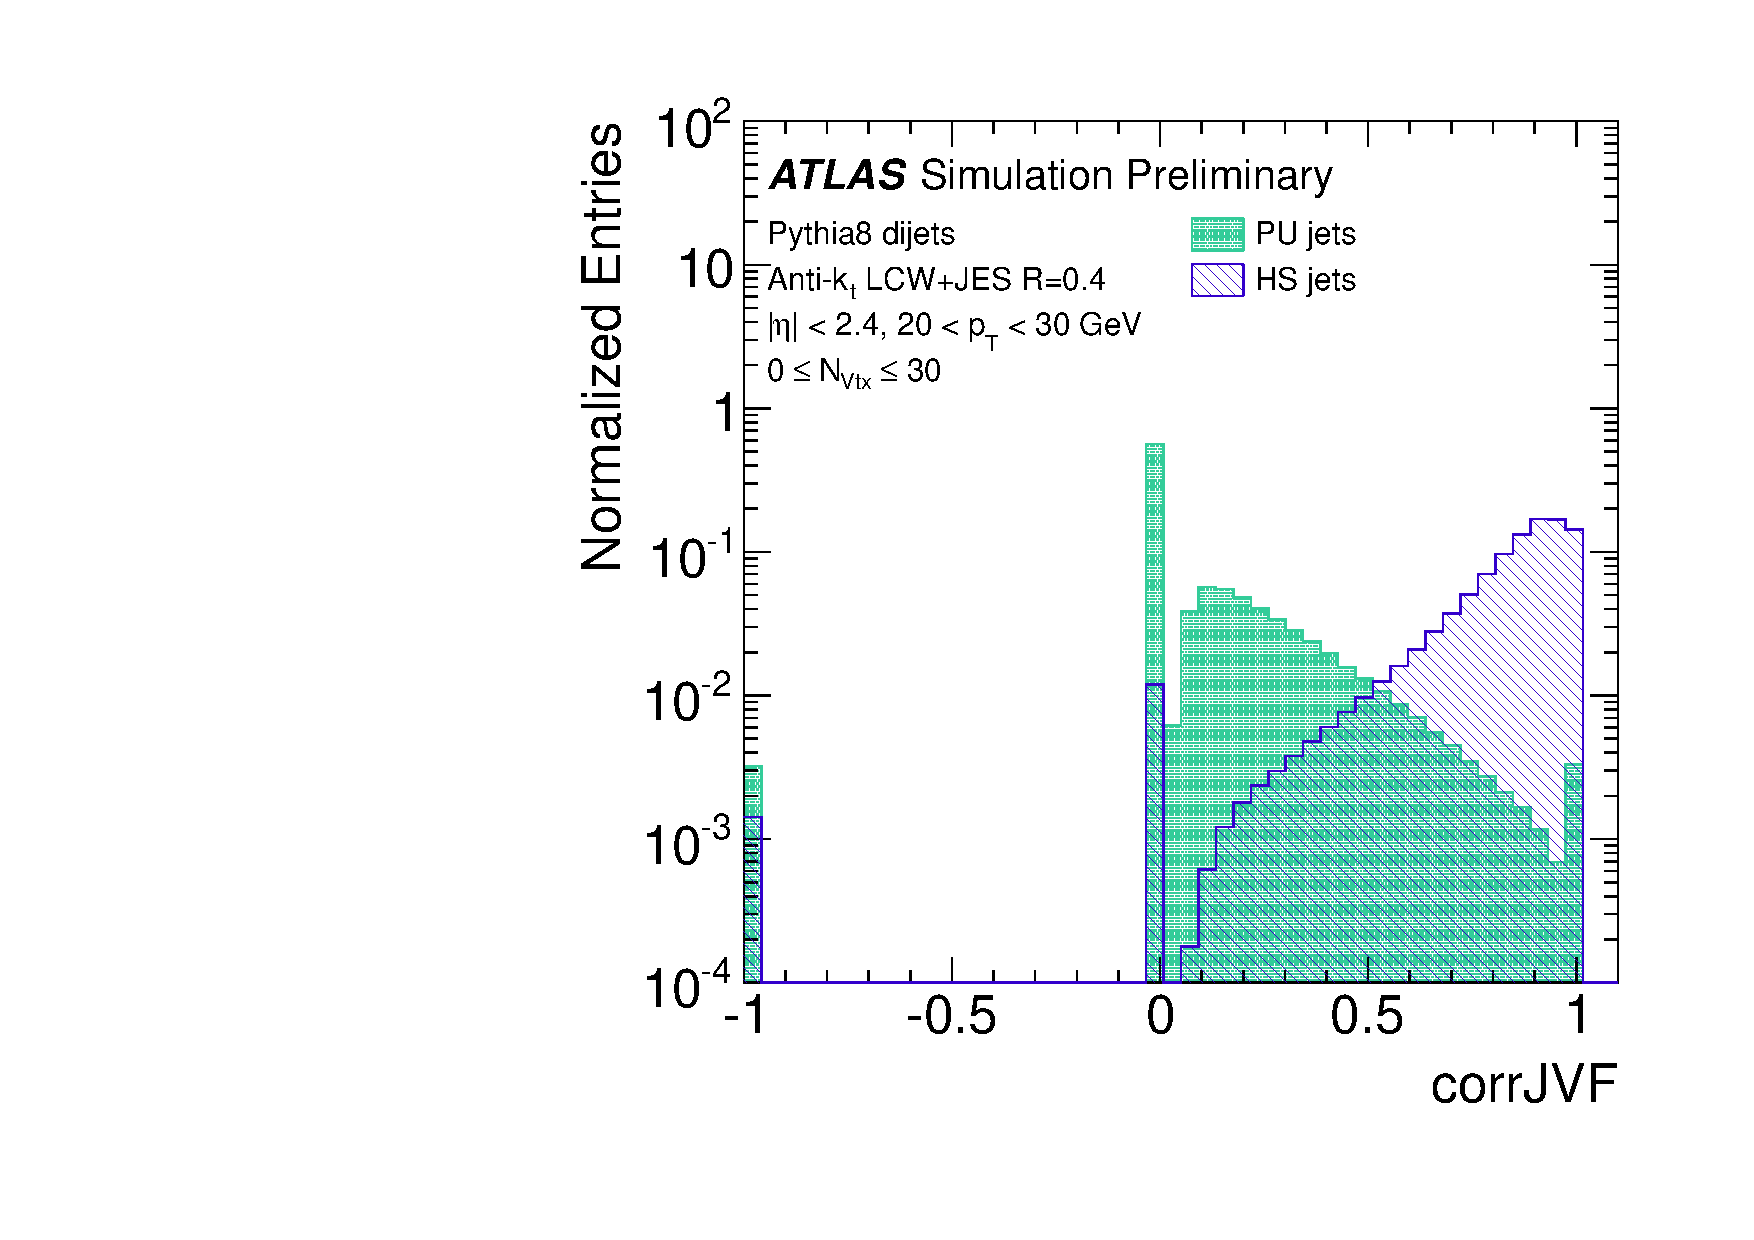
\includegraphics[width= 0.46\textwidth]{corrJVF_Distribution}
    \label{fig:corrJVF_Dist}
  }
  \subfigure[]{
      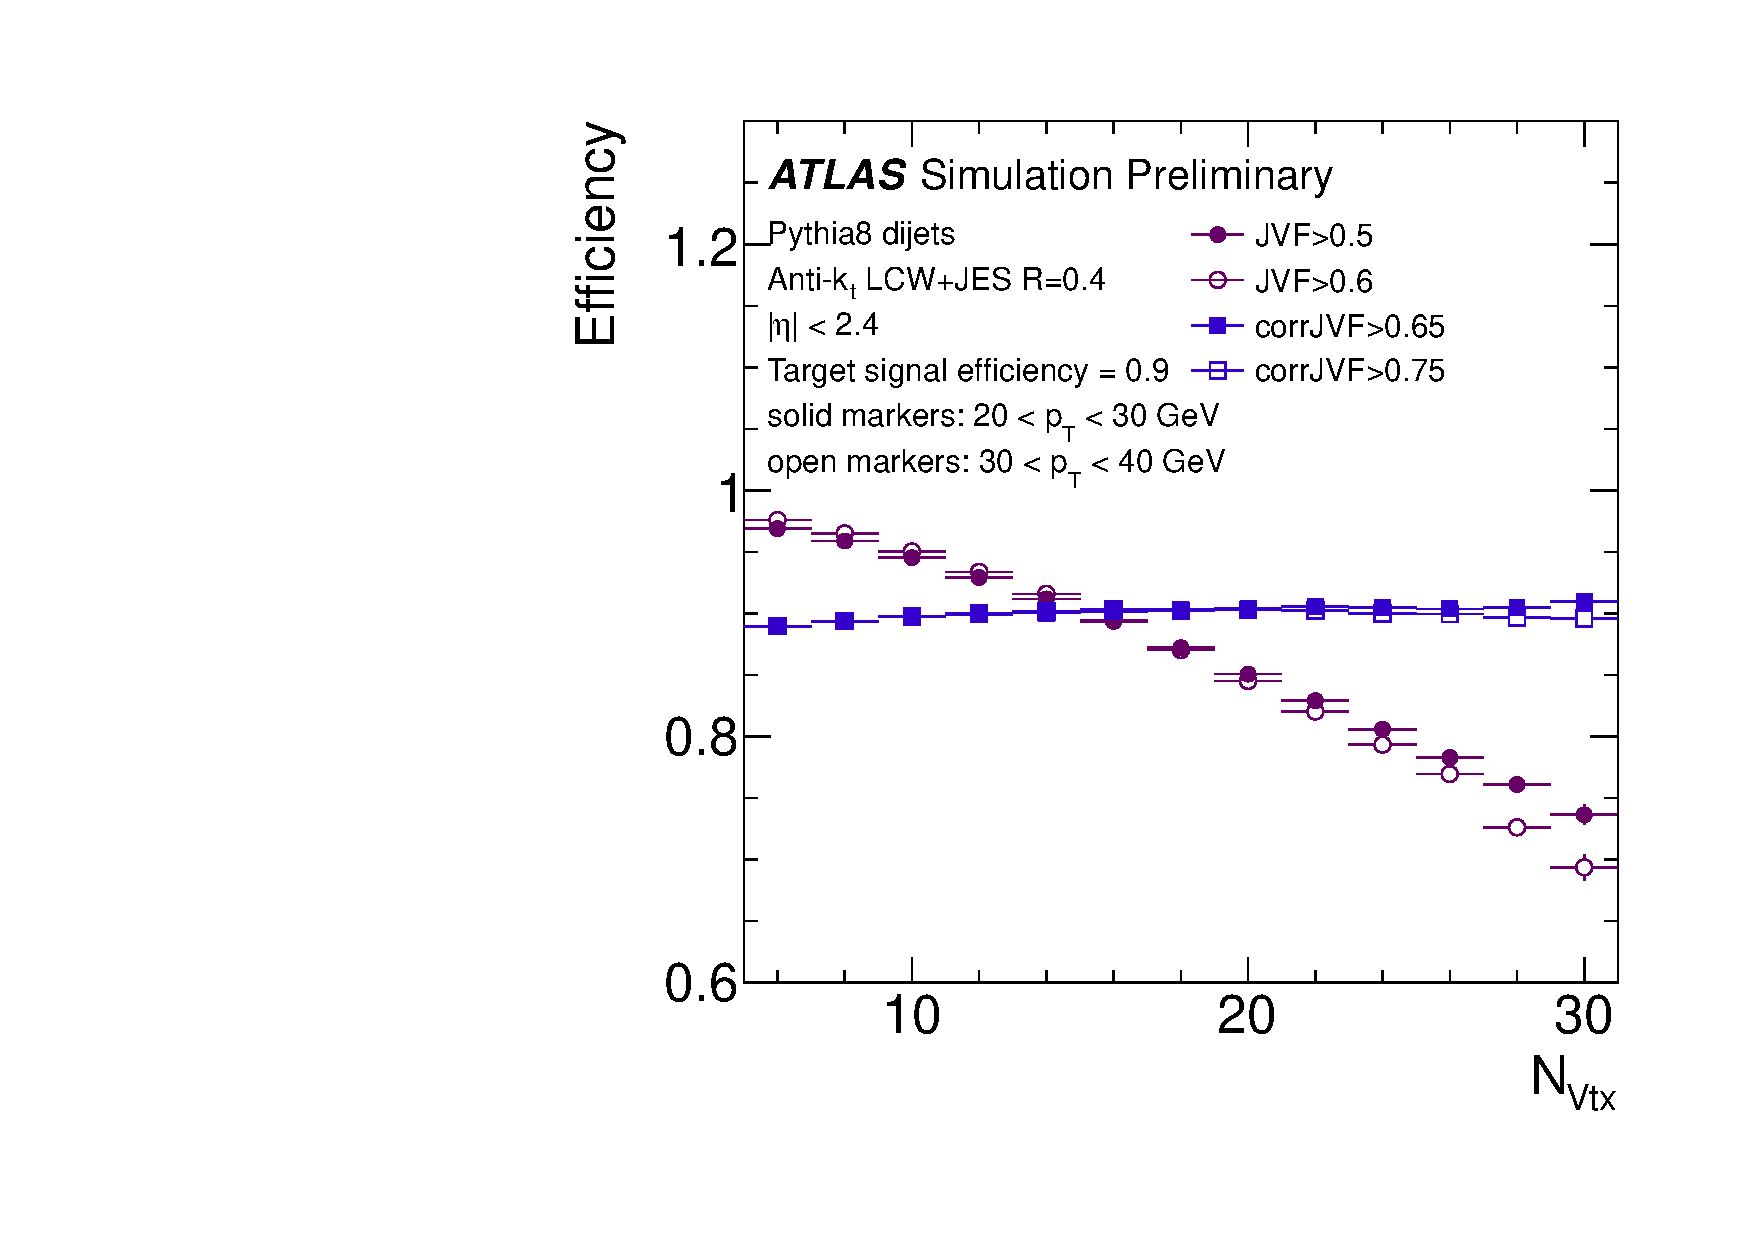
\includegraphics[width=0.46\textwidth]{corrJVFStability_eff90}
    \label{fig:corrJVF_NPVdependence}
  }
  \caption{(a) Distribution of \cJVF for pileup and hard-scatter jets with $20 < \pT < 30\GeV$. 
           (b) Primary-vertex dependence of the hard-scatter 
           jet efficiency for $20 < \pT < 30\GeV$ (solid markers) and $30 < \pT < 40\GeV$ (open markers) 
           jets for fixed cuts of \cJVF (blue) and \JVF (violet) such that the inclusive efficiency is $90\%$. 
           The cut values imposed on \cJVF and \JVF, which depend on the \pT bin, are specified in the legend.
    }
\label{fig:corrJVF}
\end{figure}
%------------------------


Figure~\ref{fig:corrJVF_Dist} shows the \cJVF distribution for pileup and hard-scatter jets in simulated dijet events. 
A value $\cJVF=-1$ is assigned to jets with no associated tracks. About $1\%$ of hard-scatter jets with $20 < \pT < 30 \GeV$ have no associated hard-scatter tracks and thus $\cJVF=0$. 
% Multiple effects may lead to pileup jets with $\cJVF=1$, such as pileup vertices merged with the hard-scatter vertex. 

Figure~\ref{fig:corrJVF_NPVdependence} shows the 
hard-scatter jet efficiency as a function of the number of 
reconstructed primary vertices in the event when imposing a minimal \cJVF or \JVF requirement such that the \NPV inclusive 
efficiency is 90\%.  
For the full range of \NPV considered, the hard-scatter jet efficiency after a selection based on \cJVF is stable at $90\%\pm1\%$, 
whereas for \JVF the efficiency degrades by about 20\%, 
from 97\% to 75\%. The choice of the scaling factor $k$ in the \cJVF distribution does not affect the stability of the hard-scatter jet efficiency with \NPV. 


\subsection{\RpT}
The variable \RpT is defined as the scalar \pT sum of the tracks that are associated with the jet and 
originate from the hard-scatter vertex divided by the fully calibrated jet \pT, which includes pileup subtraction:
%---------
\begin{equation}
\RpT = \frac{\sum_k{\pT^{{\rm trk}_k}({\rm PV}_0)}}{\pT^{jet}}.
\label{eq:RpT}
\end{equation}
%---------

\RpT is peaked at 0 and steeply falling for pileup jets, where no or only little \pT from tracks from the hard-scatter vertex is expected. 
For hard-scatter jets, however, \RpT has the meaning of a charged \pT fraction and its mean value and spread is larger than for pileup jets. Since 
\RpT involves only tracks that are associated with the hard-scatter vertex, its definition is at first order independent of \NPV.
The \RpT  distributions for pileup and hard-scatter jets are shown in Figure~\ref{fig:RpT_Dist}.
Figure~\ref{fig:RpT_NPVdependence} 
shows the hard-scatter jet efficiency as a function of \NPV 
when imposing a minimal \RpT and \JVF 
requirement such that the \NPV inclusive efficiency is $90\%$. 
For the full range of \NPV considered, the hard-scatter jet efficiency after a selection based on \RpT 
is stable at $90\%\pm1\%$.
%--------------------------
\begin{figure}[!htbp]
  \centering
  \subfigure[]{
      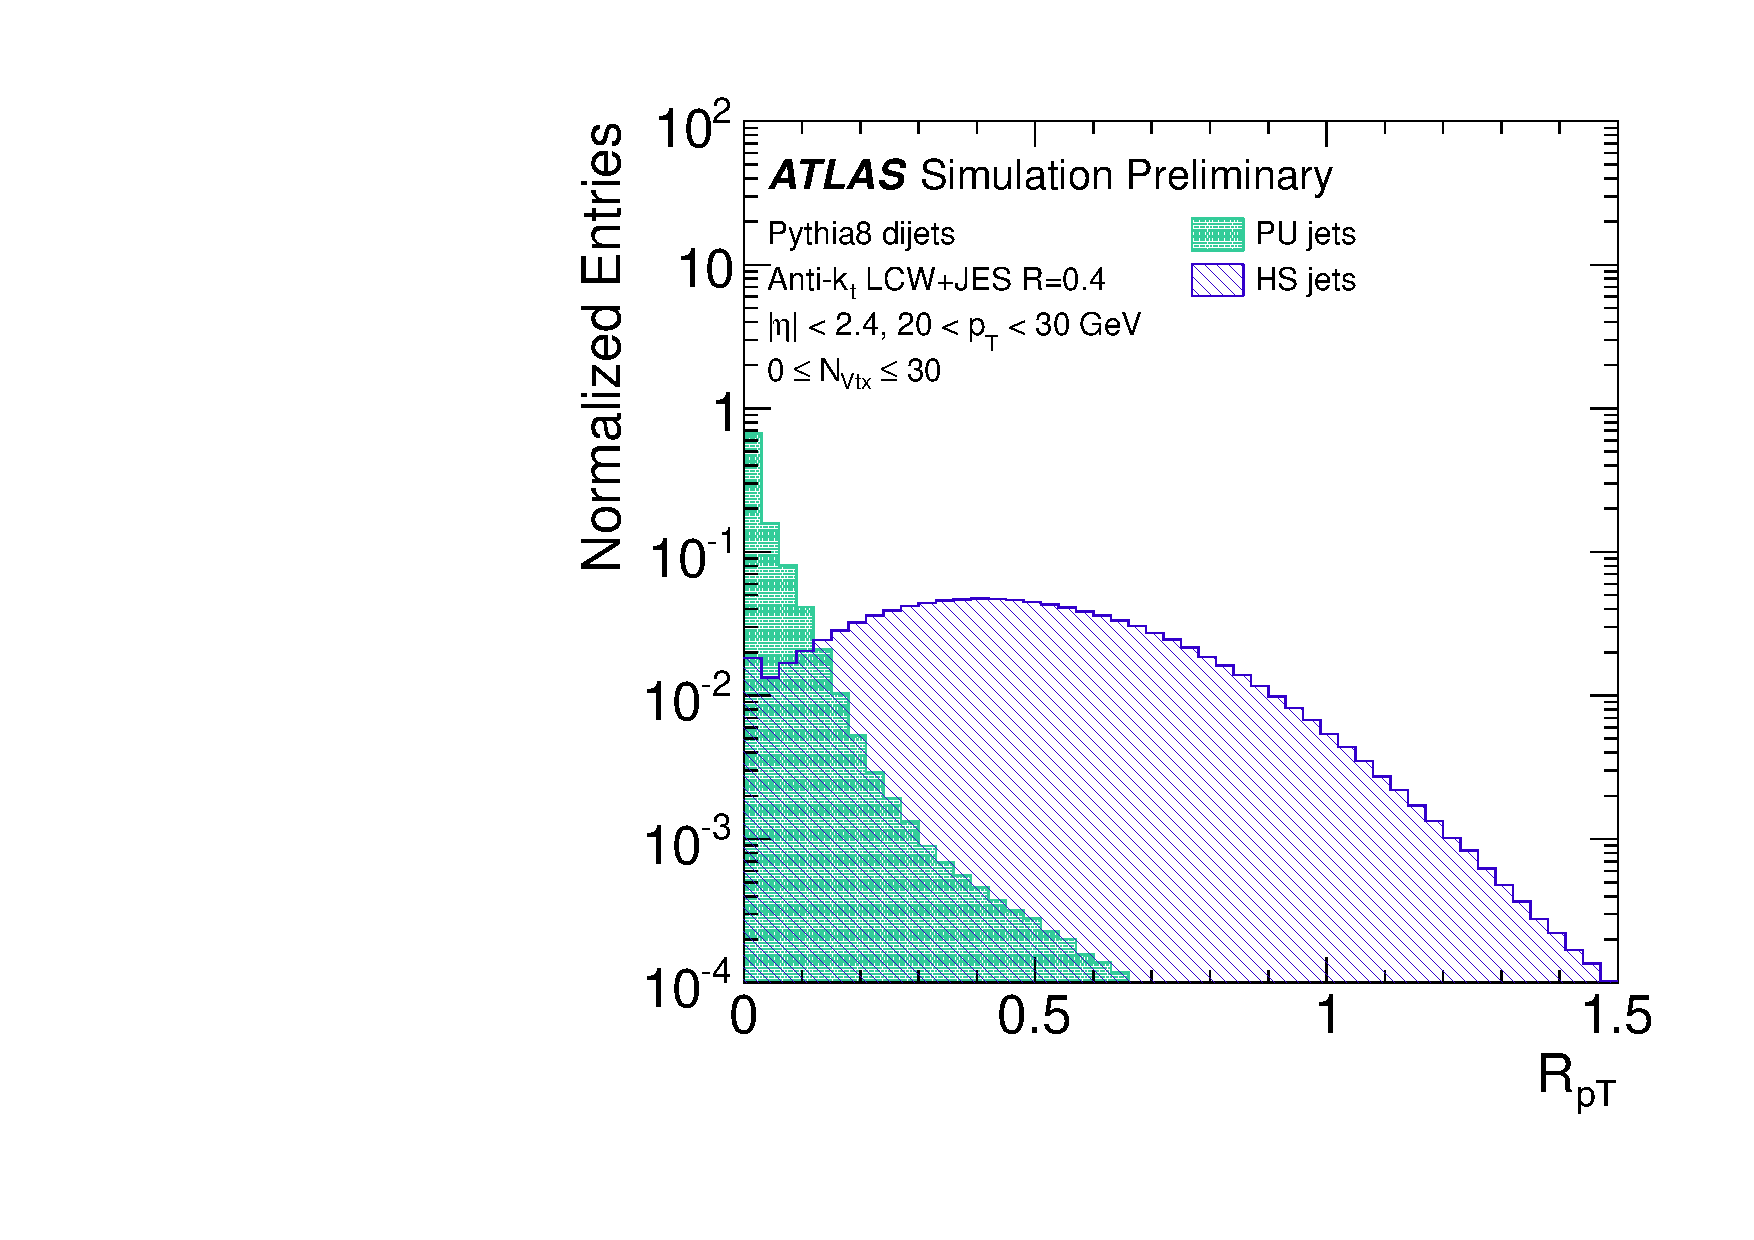
\includegraphics[width= 0.46\textwidth]{RpT_Distribution}
    \label{fig:RpT_Dist}
  }
  \subfigure[]{
      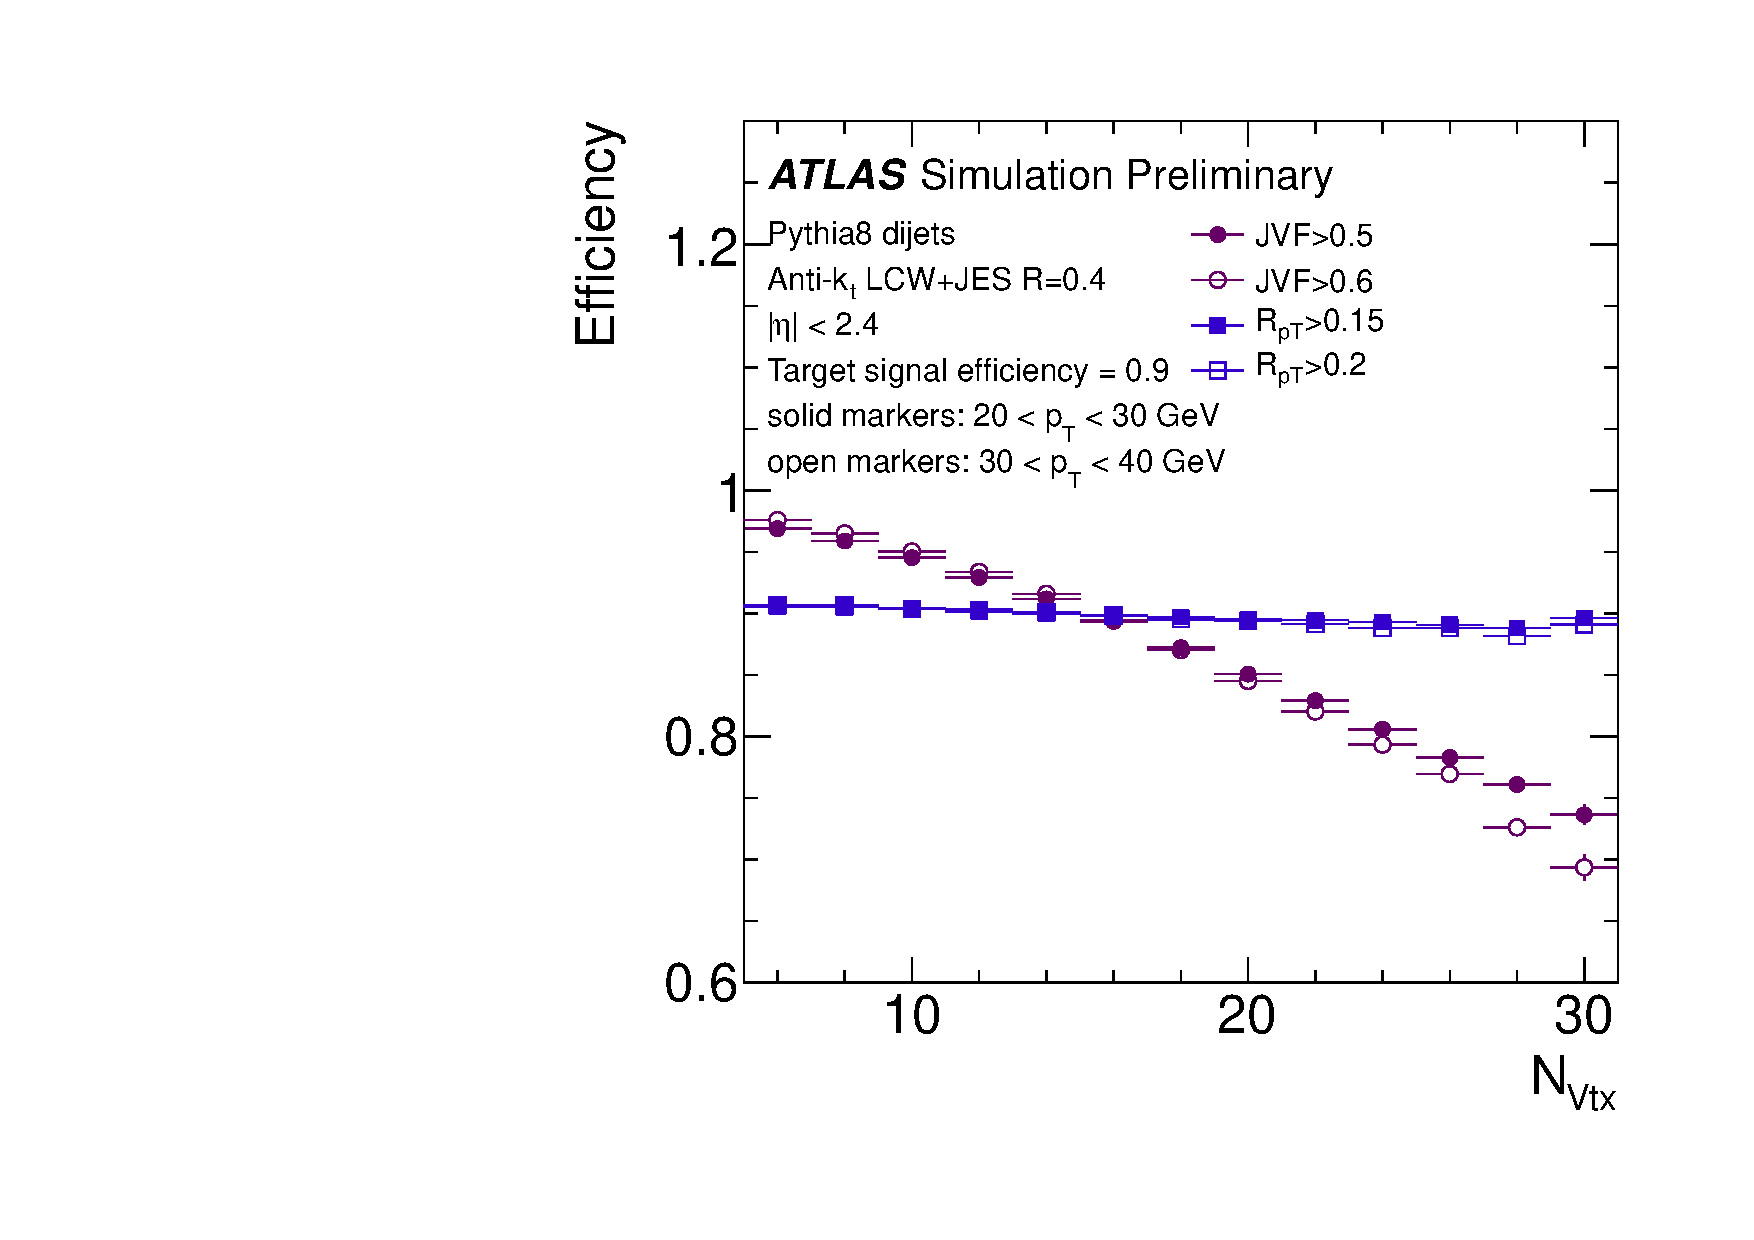
\includegraphics[width=0.46\textwidth]{RpT_Stability_eff90}
    \label{fig:RpT_NPVdependence}
  }
  \caption{(a) Distribution of \RpT for pileup and hard-scatter jets with $20 < \pT < 30\GeV$. 
           (b) Primary-vertex dependence of the hard-scatter 
           jet efficiency for $20 < \pT < 30\GeV$ (solid markers) and $30 < \pT < 40\GeV$ (open markers) 
           jets for fixed cuts of \RpT (blue) and \JVF (violet) such that the inclusive efficiency is $90\%$.
           The cut values imposed on \RpT and \JVF, which depend on the \pT bin, are specified in the legend.}

\label{fig:RpT}
\end{figure}
%------------------------




%--------------------------
\begin{figure}[!htbp]
  \centering
  \subfigure[]{
      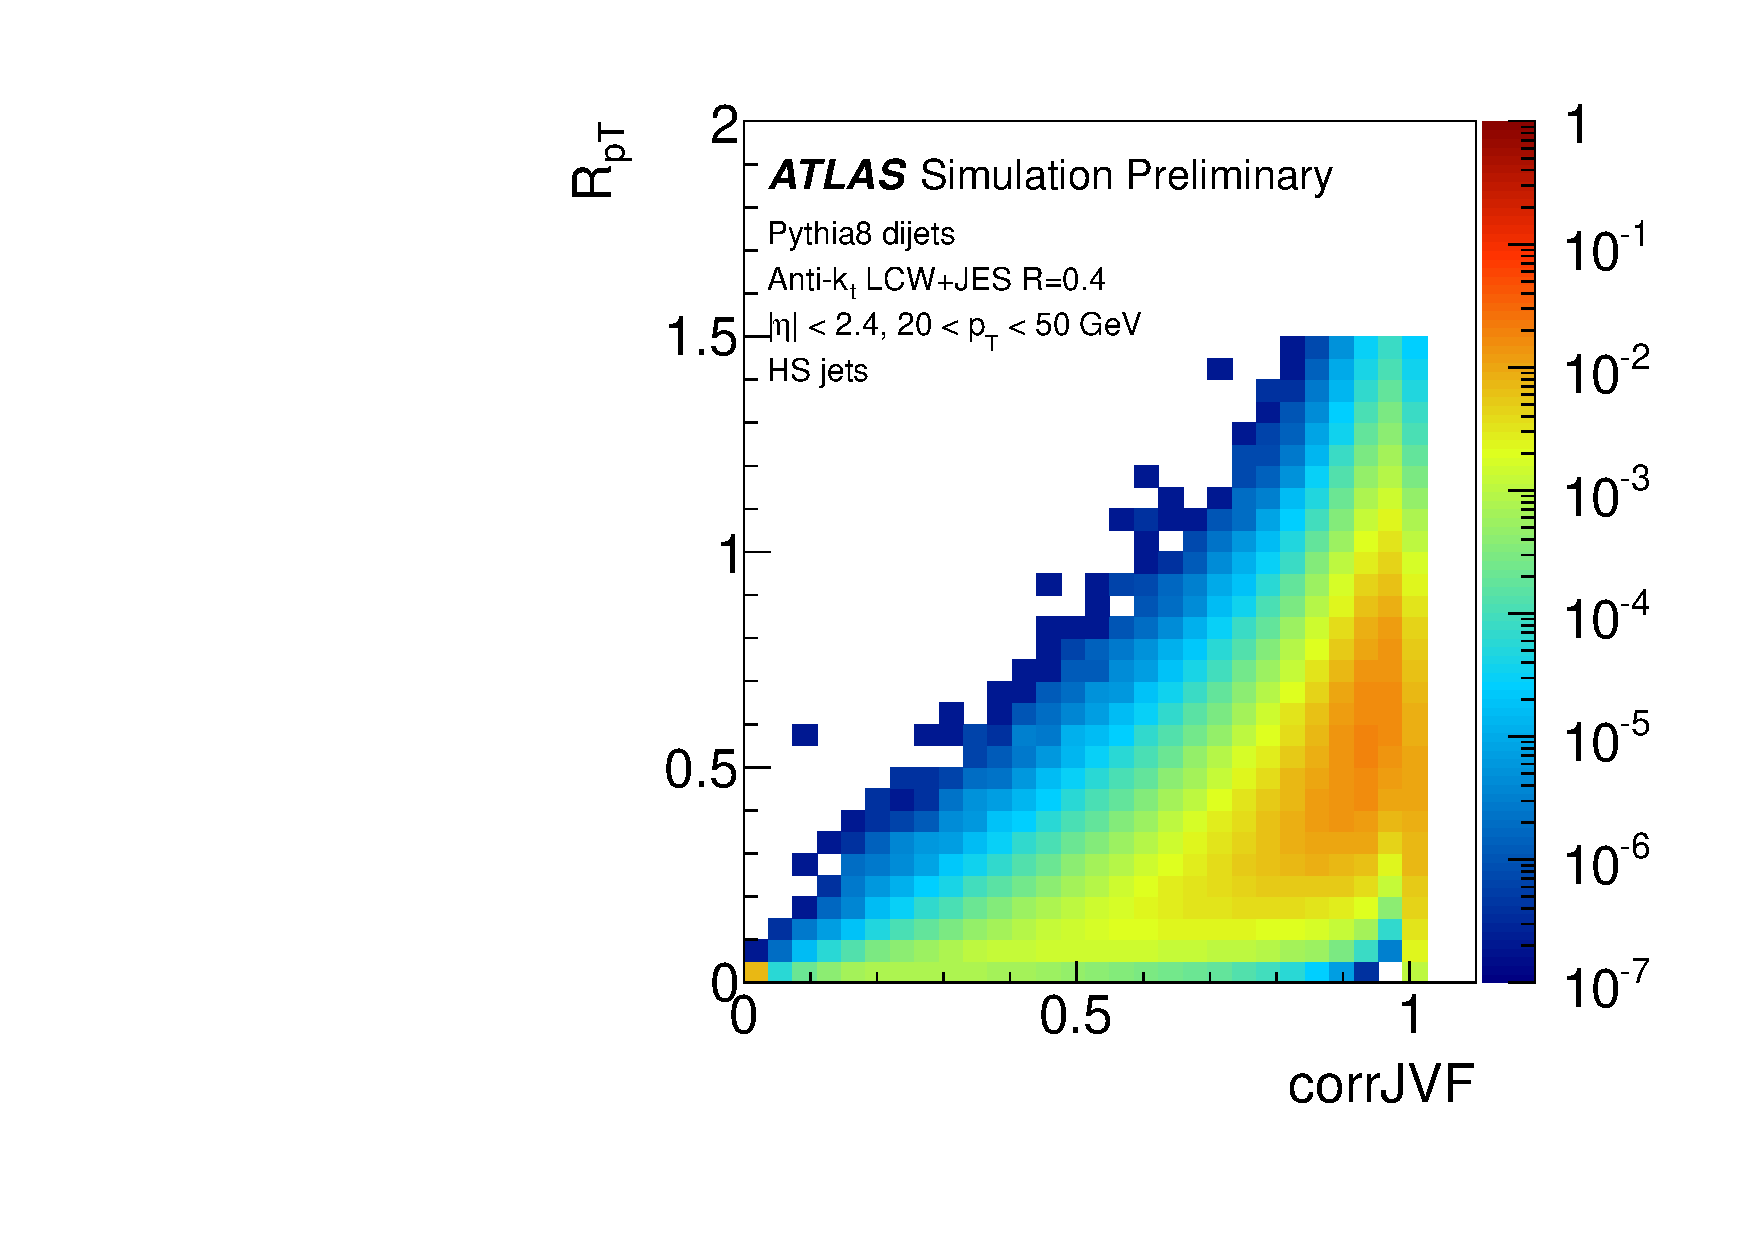
\includegraphics[width= 0.46\textwidth]{corrJVF_vs_RpT_HS}
    \label{fig:cJVF_VS_RpT_HS}
  }
  \subfigure[]{
      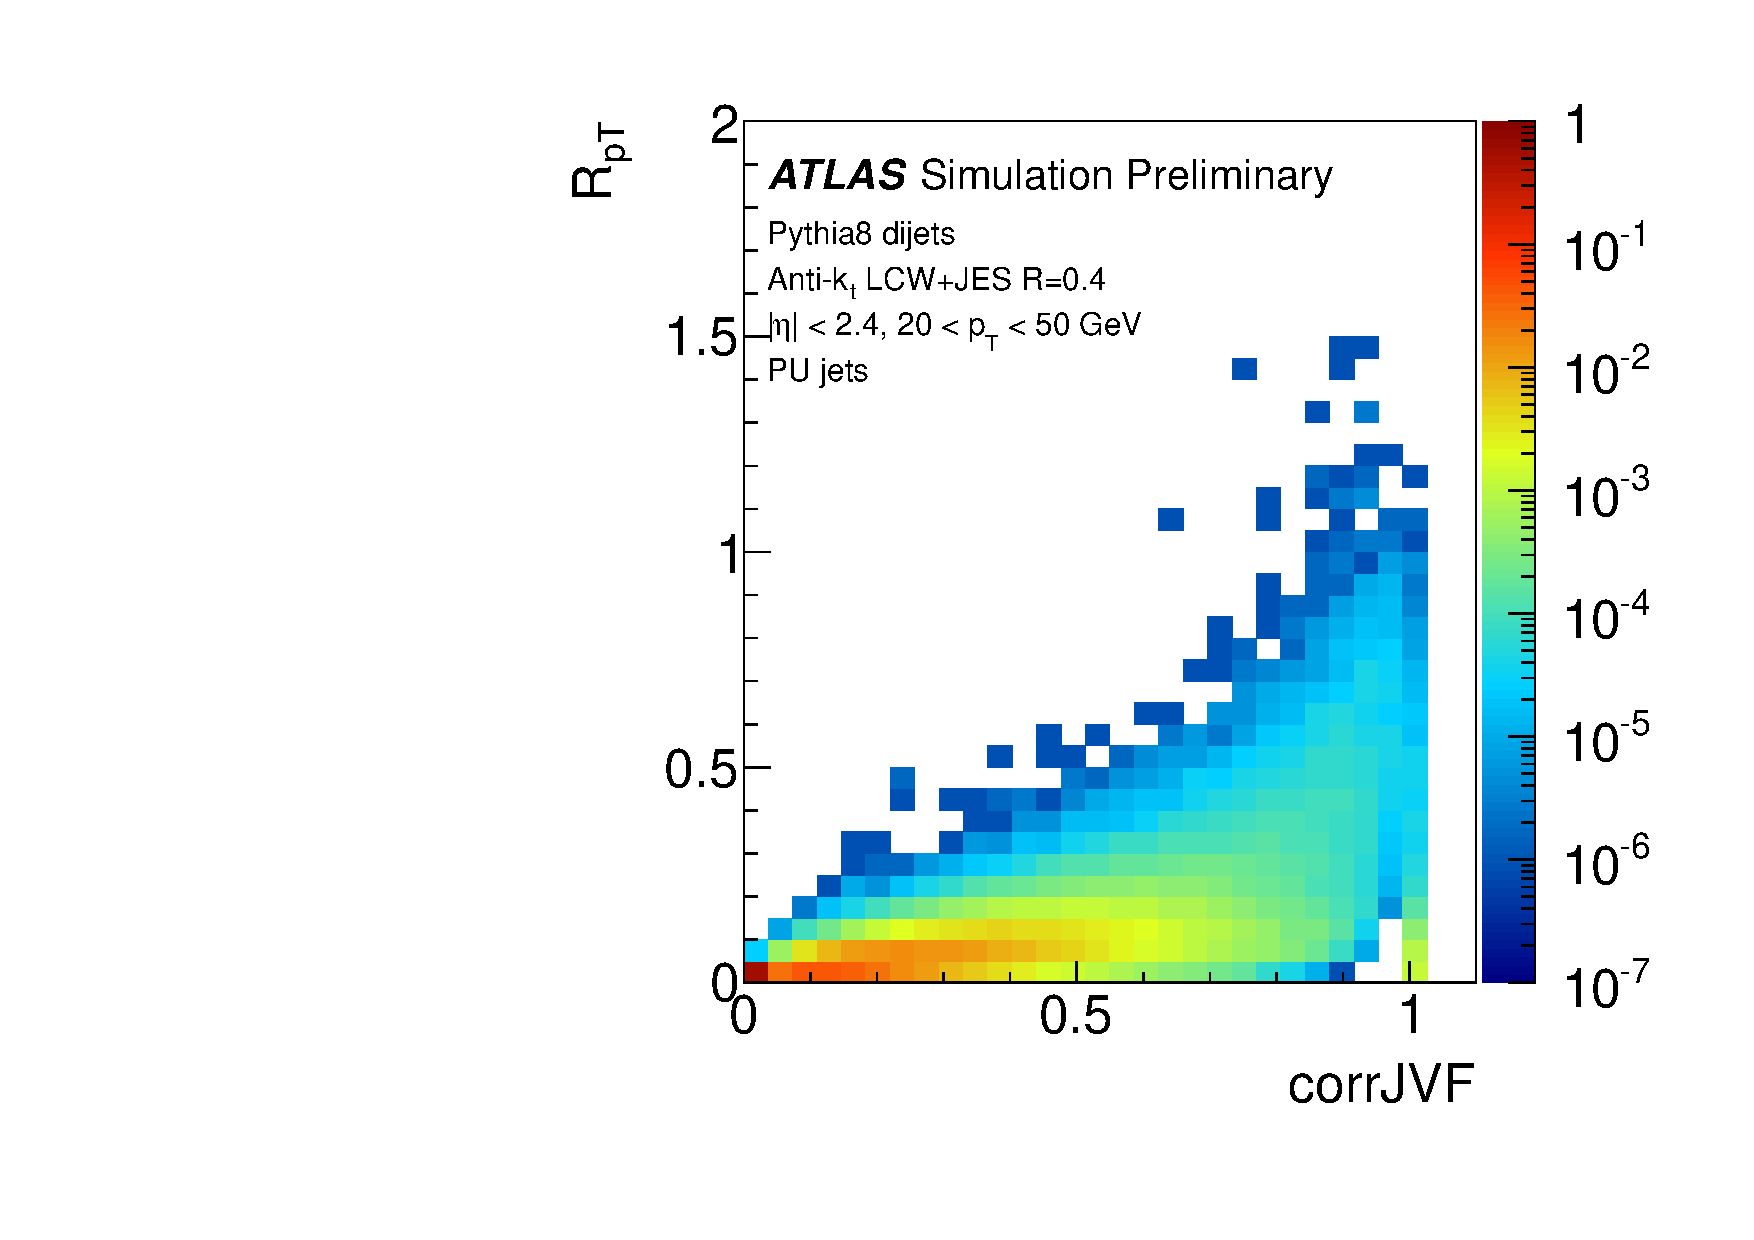
\includegraphics[width=0.46\textwidth]{corrJVF_vs_RpT_PU}
    \label{fig:cJVF_VS_RpT_PU}
  }
  \caption{2-dimensional correlation of \cJVF and \RpT for hard-scatter (a) and pileup (b) jets.}
\label{fig:cJVF_vs_RpT}
\end{figure}
%------------------------
Figures~\ref{fig:cJVF_VS_RpT_HS} and~\ref{fig:cJVF_VS_RpT_PU} show the 2-dimensional correlation of 
\RpT and \cJVF for hard-scatter and pileup jets, respectively. Hard-scatter jets are characterized by large \cJVF and 
large \RpT, whereas pileup jets are concentrated at low \RpT and low \cJVF values. 
% The correlation between these two variables holds valuable information that can be exploited when discriminating hard-scatter from pileup jets. 
Jets with $\cJVF=-1$ (\ie no associated tracks) or $\RpT >1.5$ are omitted in these plots. 
Most pileup jets (and about $1\%$ of hard-scatter jets) have no tracks that originate from the hard-scatter vertex and thus $\cJVF=\RpT=0$.




%-----------------------------------------------------------------------
\section{The jet-vertex-tagger}
\label{sec:JVT}
%--------------------------
\subsection{Derivation of the discriminant}
A new discriminant called the jet-vertex-tagger (\JVT) is constructed using \RpT and \cJVF as a 2-dimensional 
likelihood, based on a k-nearest neighbor (kNN) algorithm~\cite{Hocker:2007ht}. 
For each point in the two-dimensional $\cJVF-\RpT$ plane, the relative probability for a jet at that point to be of signal 
type is computed as the ratio of the number of hard-scatter jets divided by the number of hard-scatter plus pileup jets found in 
a local neighborhood around the point using a training sample of signal and pileup jets with $20 < \pT < 50\GeV$ and $|\eta| < 2.4$. 
The local neighborhood is defined dynamically as the 100 nearest neighbors around the test point using a Euclidean metric in the $\RpT-\cJVF$ space, where
\cJVF and \RpT are rescaled so that the variables have the same width. 
Since only based on two variables, the kNN algorithm allows for a local and straightforward calculation of the relative signal probability, 
while largely avoiding statistical fluctuations in sparsely populated regions. The resulting 2-dimensional \JVT likelihood is shown 
in Figure~\ref{fig:JVTLikelihood}.
In the following, the \JVT value of a jet is calculated, based on its \cJVF and \RpT values, using the finely binned histogram in Figure~\ref{fig:JVTLikelihood} as a lookup table.
The \JVT distribution for hard-scatter and pileup jets  with $20 < \pT < 30\GeV$ is shown in Figure~\ref{fig:JVT}. 
A value of $\JVT=-0.1$ is assigned to jets with no associated tracks. 
%---------------------
\begin{figure}[!htbp]
  \centering
  \subfigure[]{
  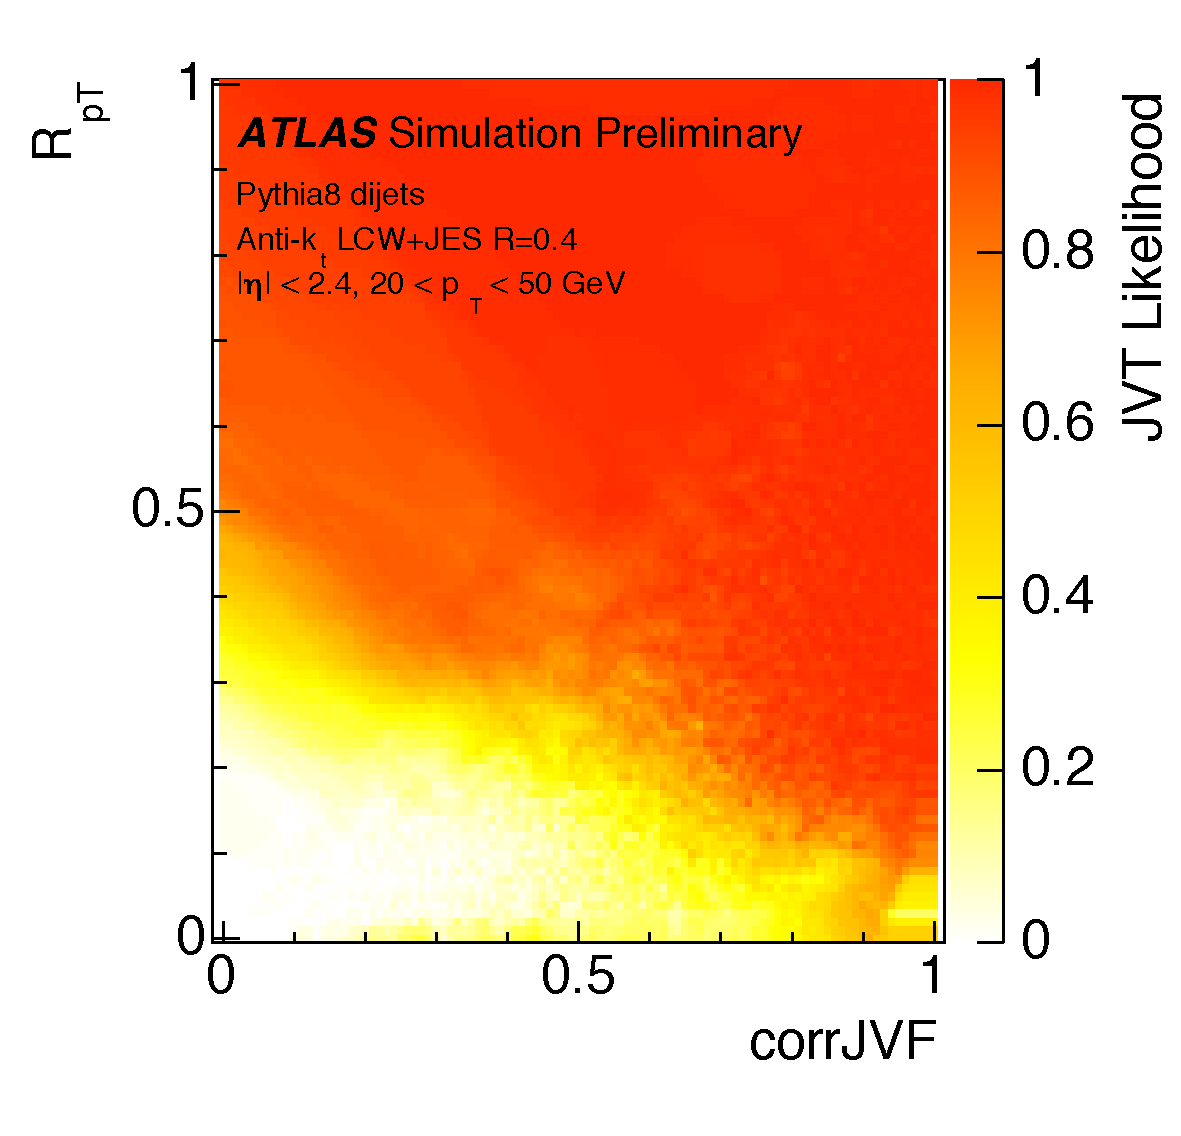
\includegraphics[width= 0.46\textwidth]{kNN100trim_pt20to50_Likelihood}
  \label{fig:JVTLikelihood}
  }
  \subfigure[]{
  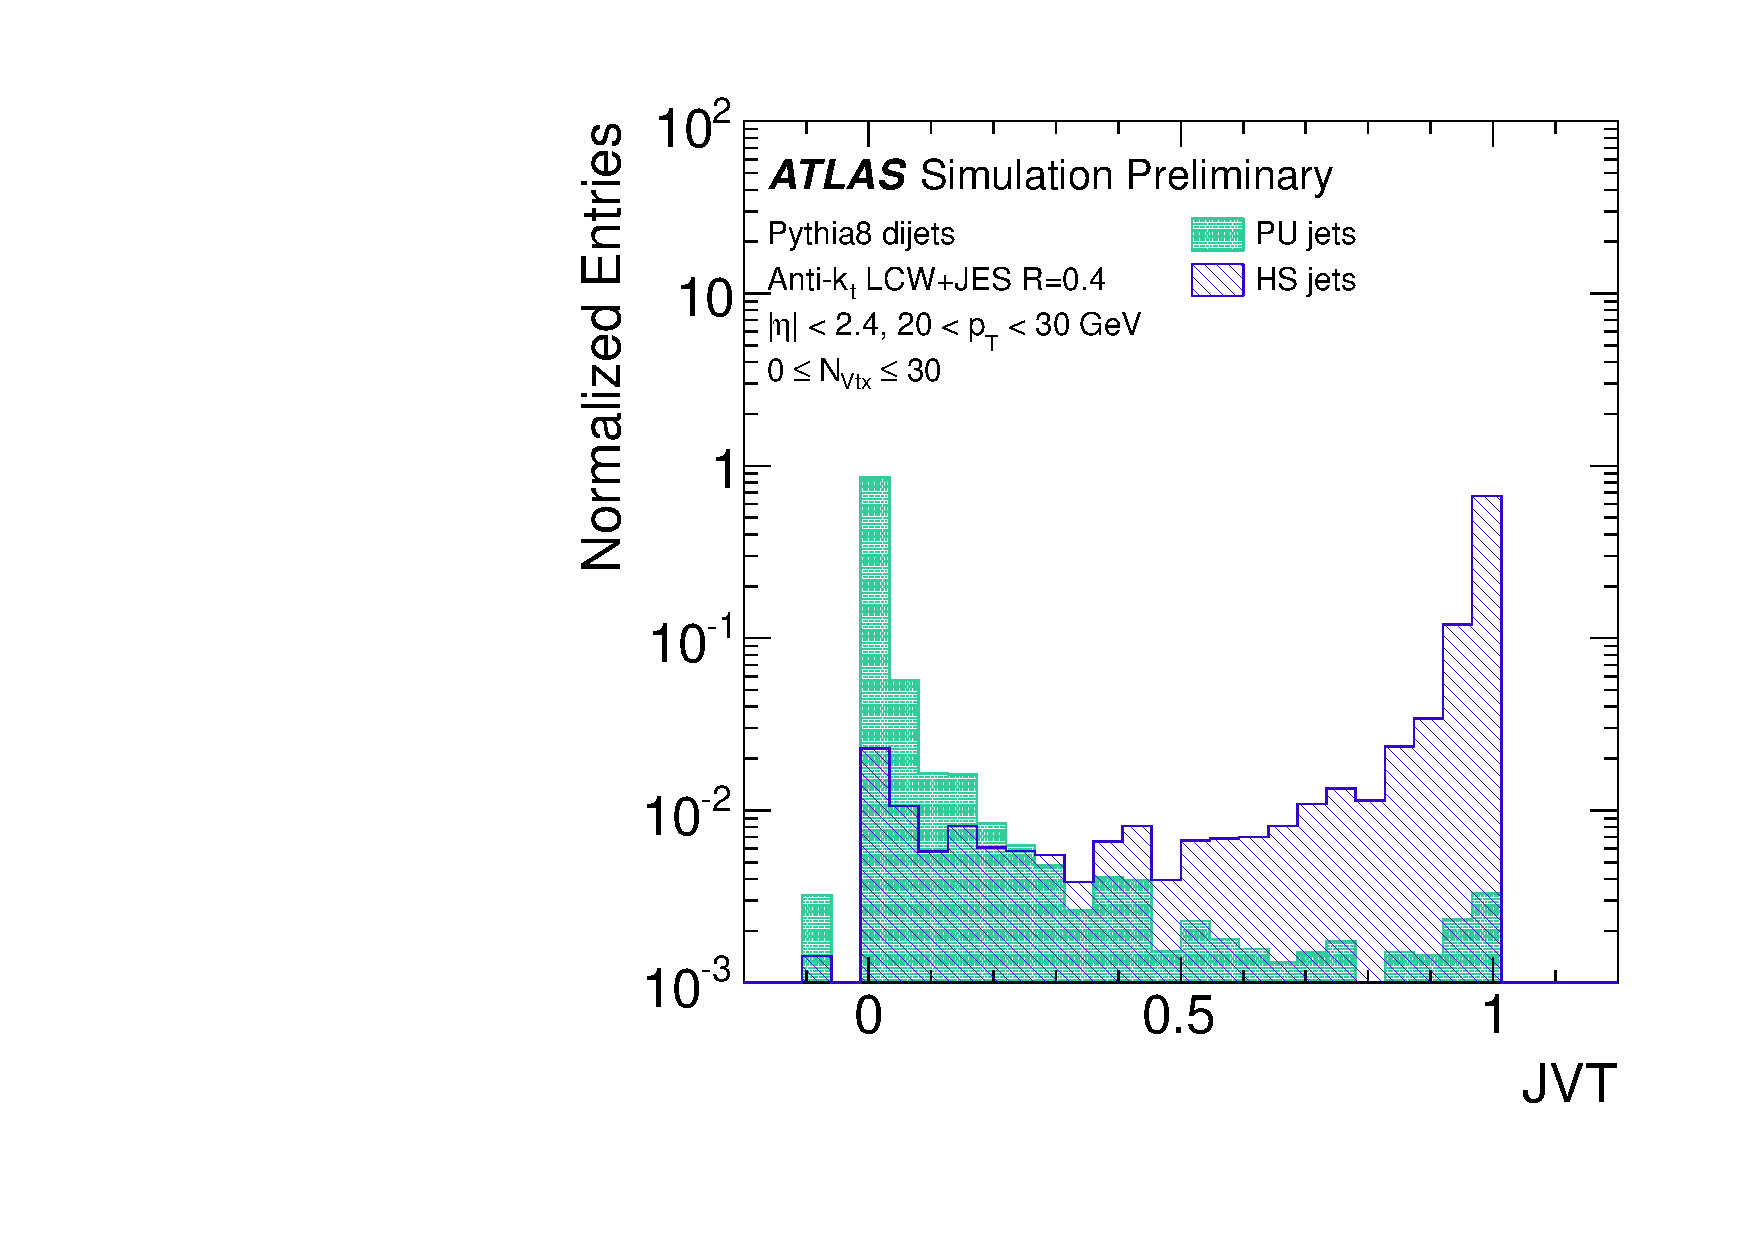
\includegraphics[width=0.46\textwidth]{JVT_distribution}
  \label{fig:JVT}
  }
  \caption{(a) The 2-dimensional \JVT likelihood as a function of \cJVF and \RpT. Jets with $\cJVF=-1$ (\ie no associated tracks) are omitted in this figure.
      Jets with $\RpT >1$ have $\JVT$ from 0.98 to 1 and are not included in the figure.
     (b) Distribution of \JVT for pileup and hard-scatter jets with $20 < \pT < 30\GeV$.}
\end{figure}
%------------------------

To test the sample dependence of \JVT, the likelihood is also derived using a sample of $20 < \pT < 50\GeV$ jets in simulated $\Zboson(\to\mu\mu)$+jets
events. The performance of the \JVT-based pileup jet suppression (evaluated in terms of fake rate \vs efficiency curves) is found not to significantly depend
on the sample from which the likelihood is derived. These studies are reported in Appendix~\ref{app:sample_dep}.


% %---------------------
% \begin{figure}[!htbp]
%   \centering
%   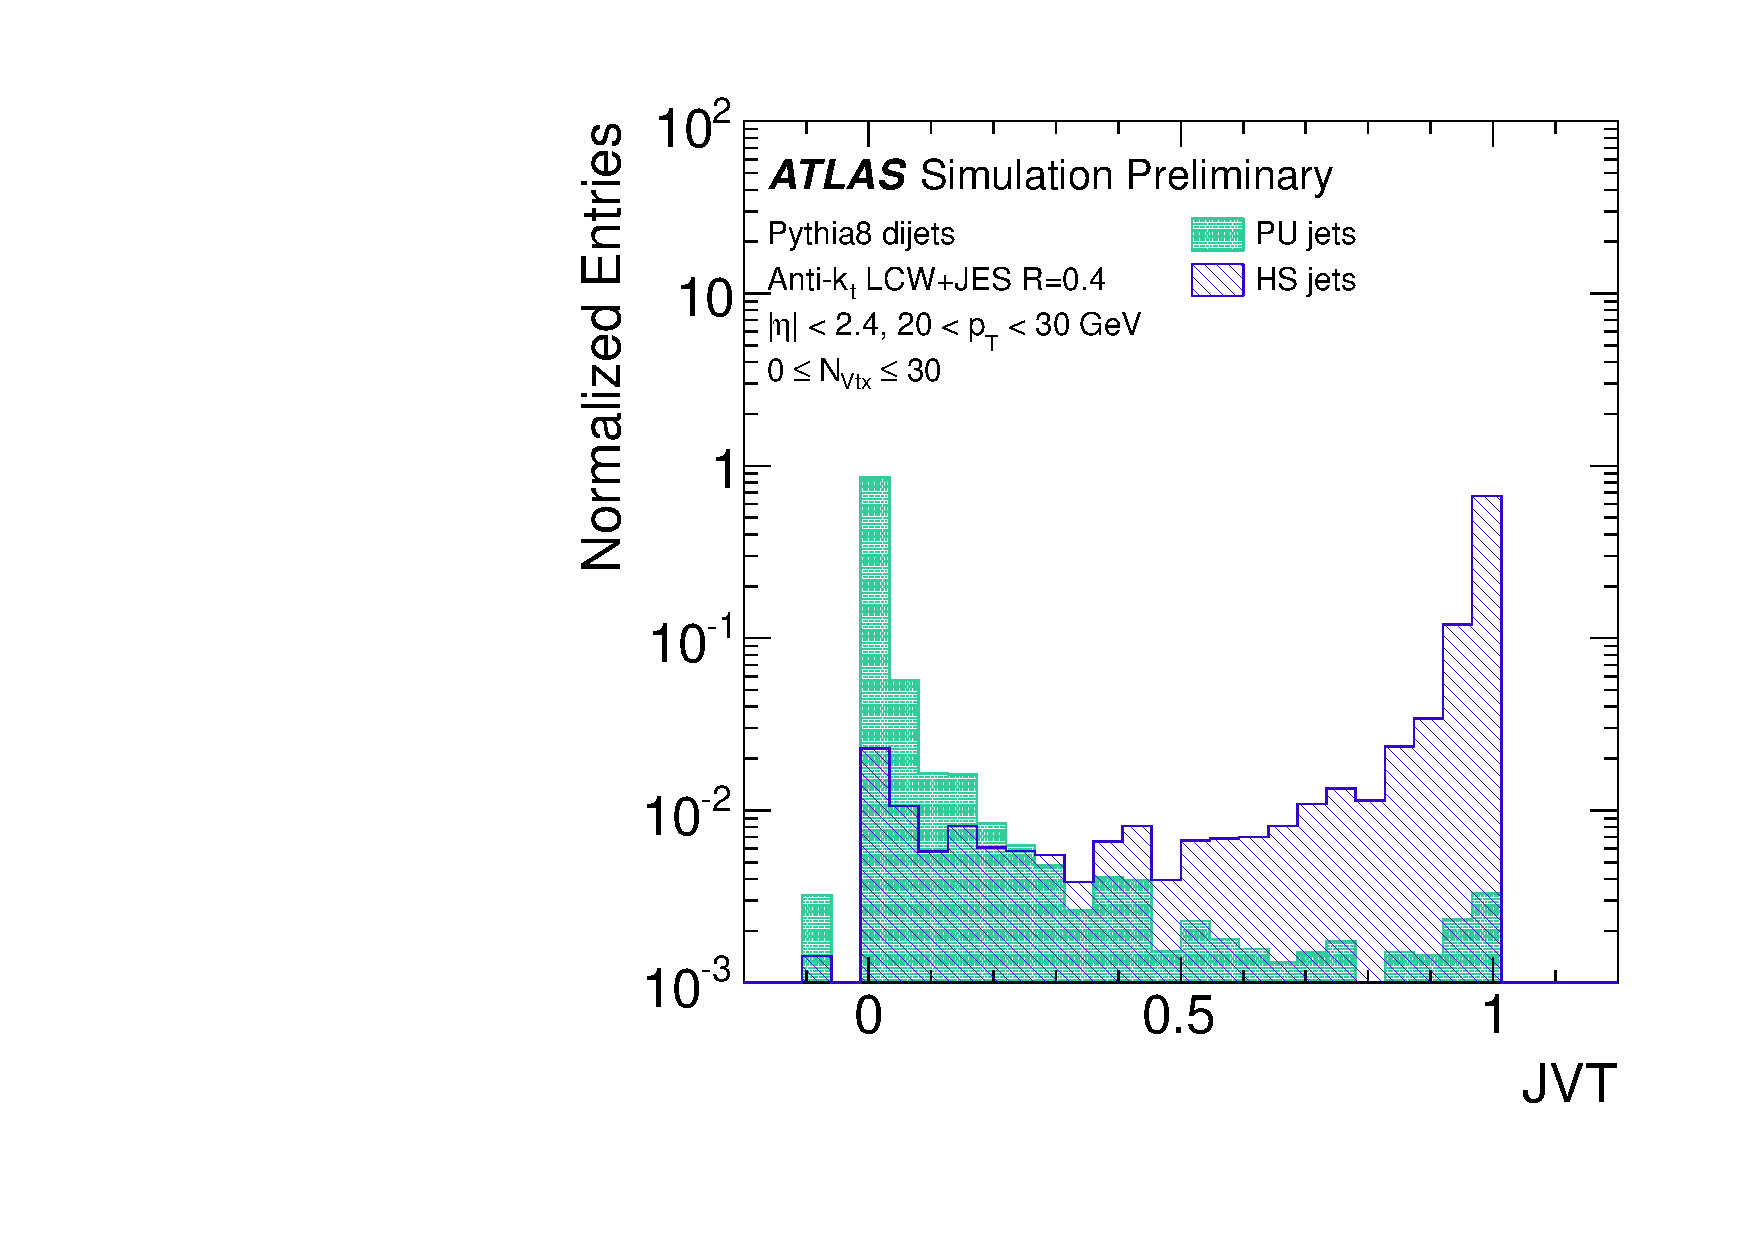
\includegraphics[width=0.46\textwidth]{JVT_distribution}
%   \caption{Distribution of \JVT for pileup and hard-scatter jets with $20 < \pT < 30\GeV$.}
%   \label{fig:JVT}
% \end{figure}
% %------------------------


%-----------------------------------------------------------------------------------------------------------------------------
\subsection{Performance of the \JVT-based pileup jet rejection}
Figure~\ref{fig:ROC} shows the fake rate versus efficiency curves comparing 
the performance of the four variables \JVF%
\footnote{The \JVF definition used here is the one of Ref.~\cite{ATLASConfNote:PUcorrection} (\ie based on a different track-to-vertex association), to 
allow for a direct comparison of the performance of the pileup jet suppression between this note and Ref.~\cite{ATLASConfNote:PUcorrection}.}
%
, \cJVF, \RpT, and \JVT when selecting a sample of 
jets with $20 < \pT < 50\GeV$, $|\eta|<2.4$ 
%and at least one associated track 
in simulated dijet events.
%--------------------------
\begin{figure}[!htbp]
  \centering
  \subfigure[]{
  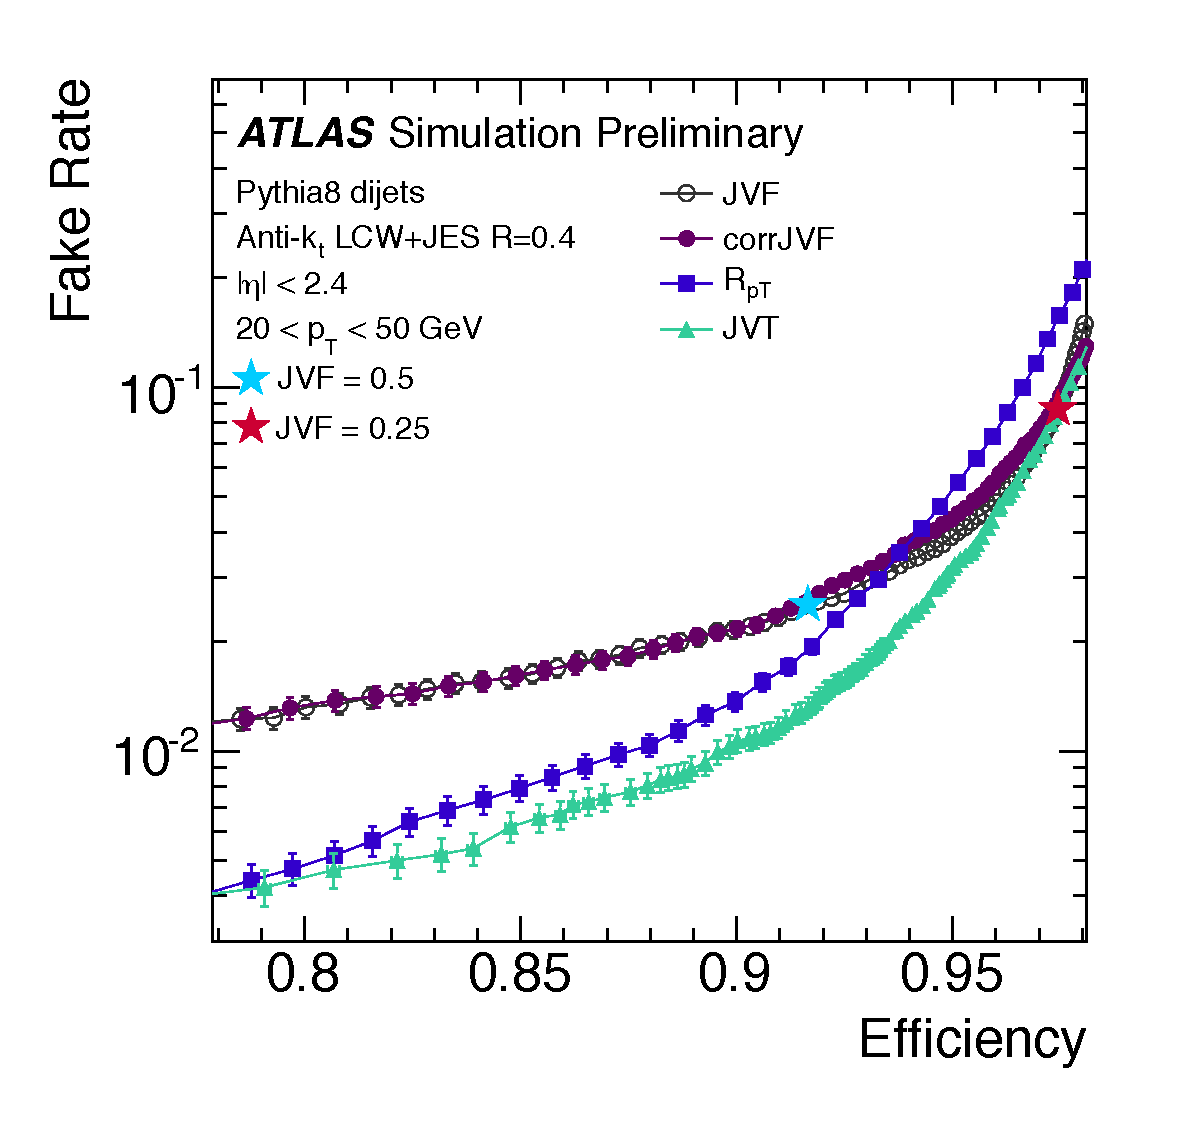
\includegraphics[width= 0.46\textwidth]{ROC_pt20to50_markers}
%  \includegraphics[width= 0.46\textwidth]{ROC_pt20to50}
  \label{fig:ROC}
  }
  \subfigure[]{
  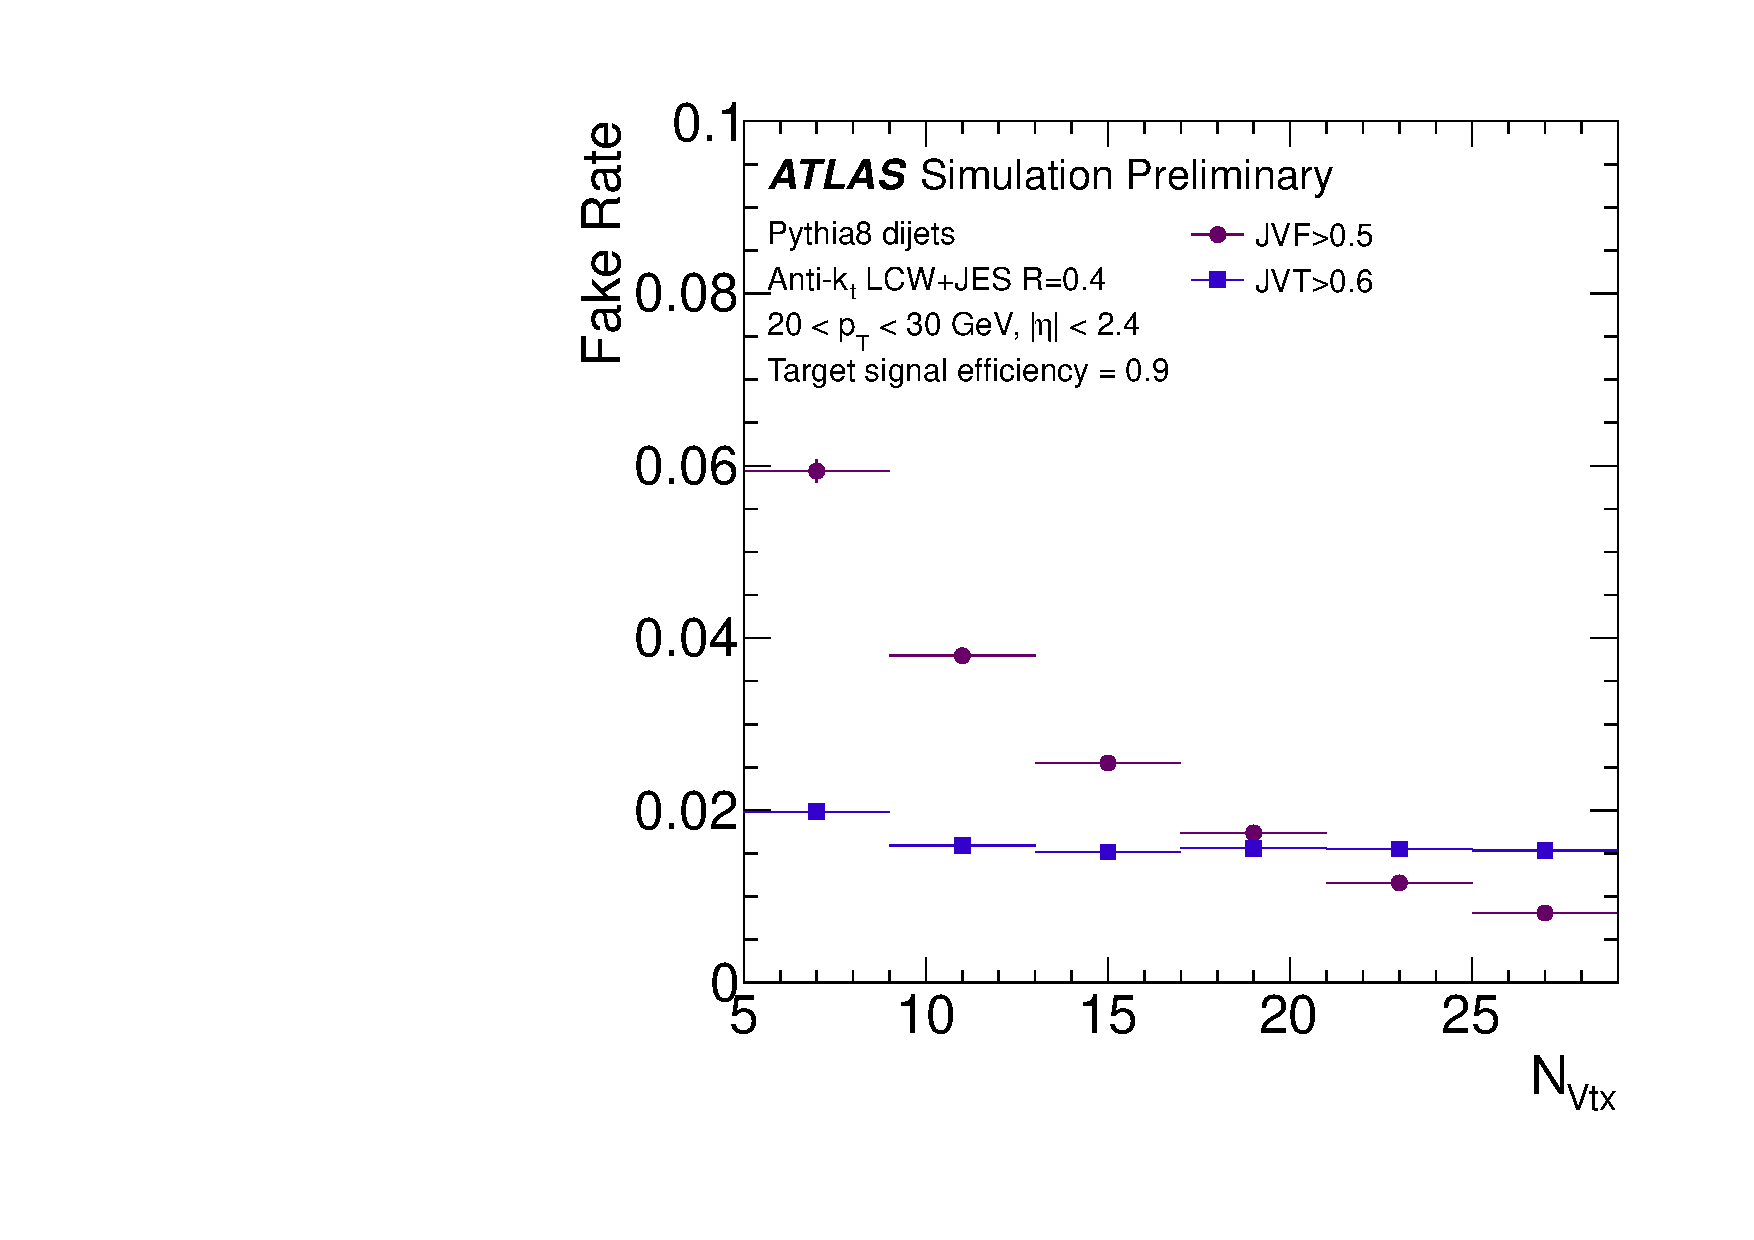
\includegraphics[width= 0.46\textwidth]{JVT_FakeRate_vs_NPV_vs_JVF_pt20to30}
  \label{fig:JVT_fakerate}
  }
  \caption{(a) Fake rate from pileup jets versus hard-scatter jet efficiency curves for \JVF, \cJVF, \RpT, and \JVT. 
  The widely used \JVF working points with cut values $0.25$ and $0.5$ are indicated with red and blue stars. 
  (b) \NPV dependence of the pileup jet fake rate when imposing cuts on \JVT (blue) and \JVF (violet) such that the inclusive hard-scatter jet efficiency is $90\%$.
  } 
\end{figure}
%------------------------
% The $0.1\%$ ($0.3\%$) of hard-scatter (pileup) jets with no associated tracks are excluded.
The figure shows the fraction of pileup jets 
passing a minimal \JVF, \cJVF, \RpT or \JVT requirement as a function of the signal jet efficiency 
resulting from the same requirement. The \JVT performance is driven by \cJVF (\RpT) in the region of high 
signal jet efficiency (high pileup rejection). Using \JVT, signal jet efficiencies of $80\%$, $90\%$ and $95\%$ are achieved for pileup fake 
rates of respectively $0.4\%$, $1.0\%$ and $3\%$. When imposing cuts on \JVF that result in the same jet efficiencies, the pileup fake rates are $1.3\%$, $2.2\%$ and $4\%$. 

% -----------------------------------------------------------------------------------------------------------------------------
% \subsection{\NPV and $\mu$ dependence of \JVT}
Figure~\ref{fig:JVT_fakerate} shows the pileup jet fake rate as a function of the number of reconstructed primary vertices in the event
when imposing a minimal \JVT and \JVF requirement such that the \NPV inclusive efficiency is $90\%$. While for \JVT the 
fake rate is stable, a decreasing trend with  \NPV is observed for \JVF, due to the pileup dependent denominator in the \JVF definition 
(see \Eqref{eq:JVF}). 

The dependence of the hard-scatter jet efficiencies on \NPV is shown in Figure~\ref{fig:fig:JVT_stab_90}, when imposing the same \JVF and \JVT cuts as in 
Figure~\ref{fig:JVT_fakerate}. In Figure~\ref{fig:fig:JVT_stab_95} looser cut values are used, resulting in \NPV inclusive hard-scatter jet efficiencies of $95\%$.
For the full range of \NPV considered, the hard-scatter 
jet efficiencies after a selection based on \JVT are stable within $1\%$.
Figure~\ref{fig:JVT_stab_mu} is similar to Figure~\ref{fig:JVT_stab} but instead shows the hard-scatter jet efficiencies as a function of 
the average number of interactions per bunch crossing $\mu$. 

%---------------------
\begin{figure}[!htbp]
  \centering
  \subfigure[]{
  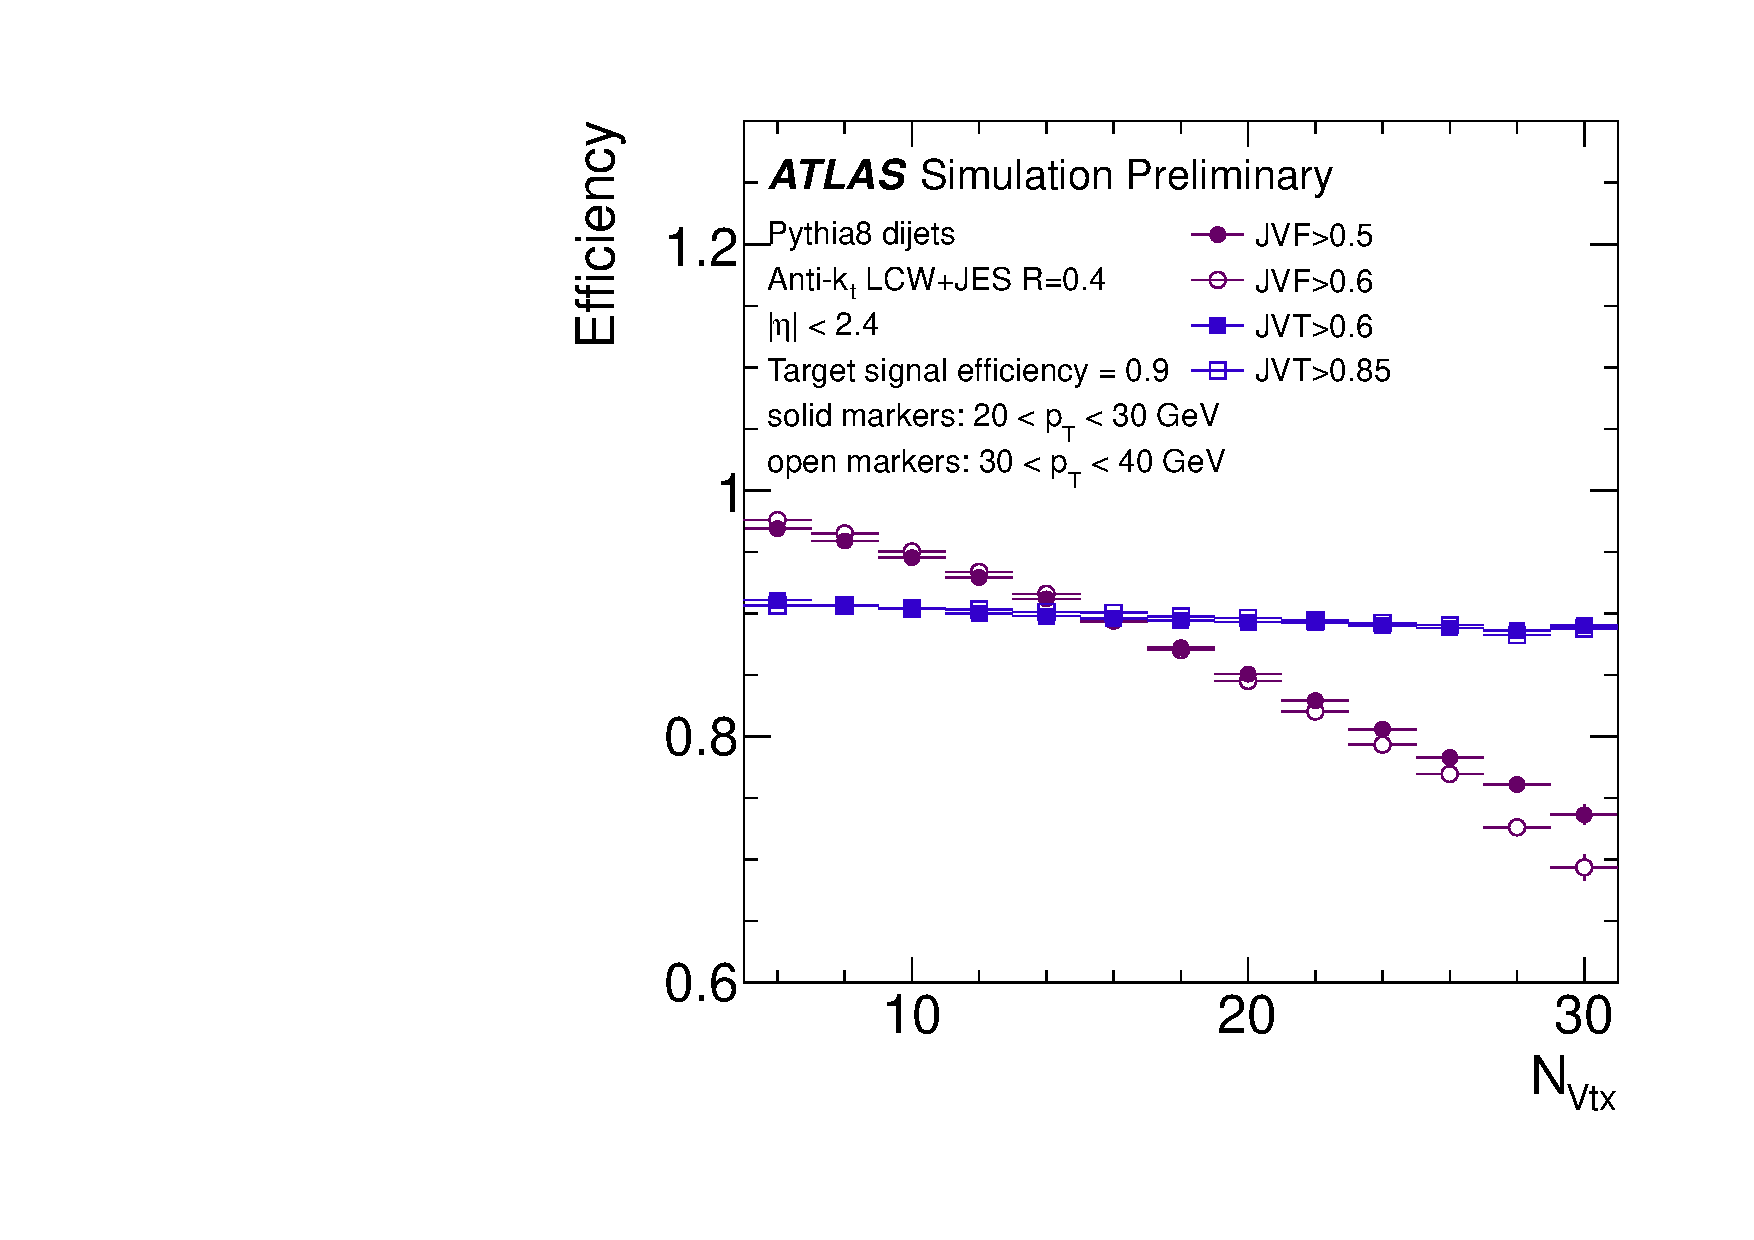
\includegraphics[width= 0.46\textwidth]{JVT_stability_eff90}
  \label{fig:fig:JVT_stab_90}
  }
  \subfigure[]{
  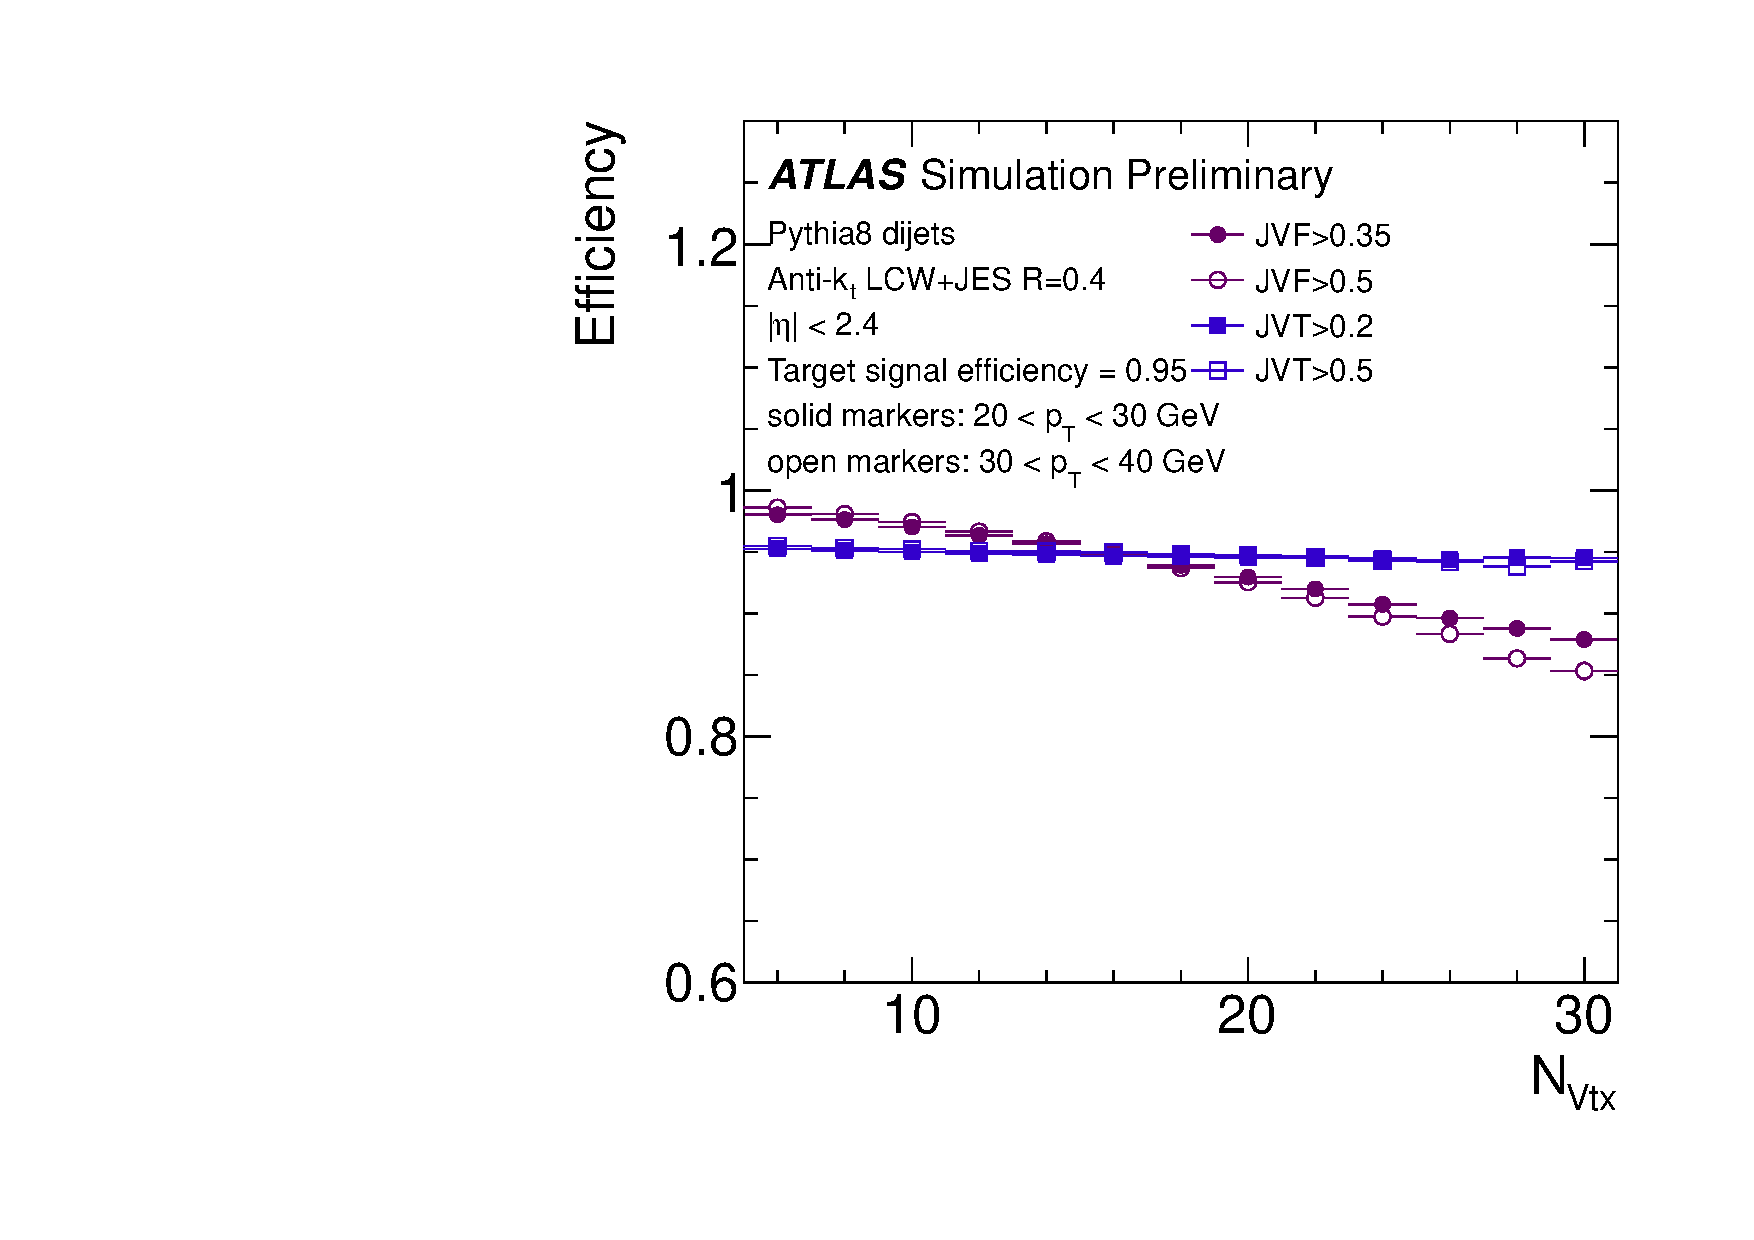
\includegraphics[width= 0.46\textwidth]{JVT_stability_eff95}
  \label{fig:fig:JVT_stab_95}
  }
  \caption{Primary-vertex dependence of the hard-scatter 
           jet efficiency for $20 < \pT < 30\GeV$ (solid markers) and $30 < \pT < 40\GeV$ (open markers) 
           jets for fixed cuts of \JVT (blue) and \JVF (violet) such that the inclusive efficiency is $90\%$ (a) and $95\%$ (b).
           The cut values imposed on \JVT and \JVF, which depend on the \pT bin, are specified in the legend.}
  \label{fig:JVT_stab}
  % new figure 
  \centering
  \subfigure[]{
  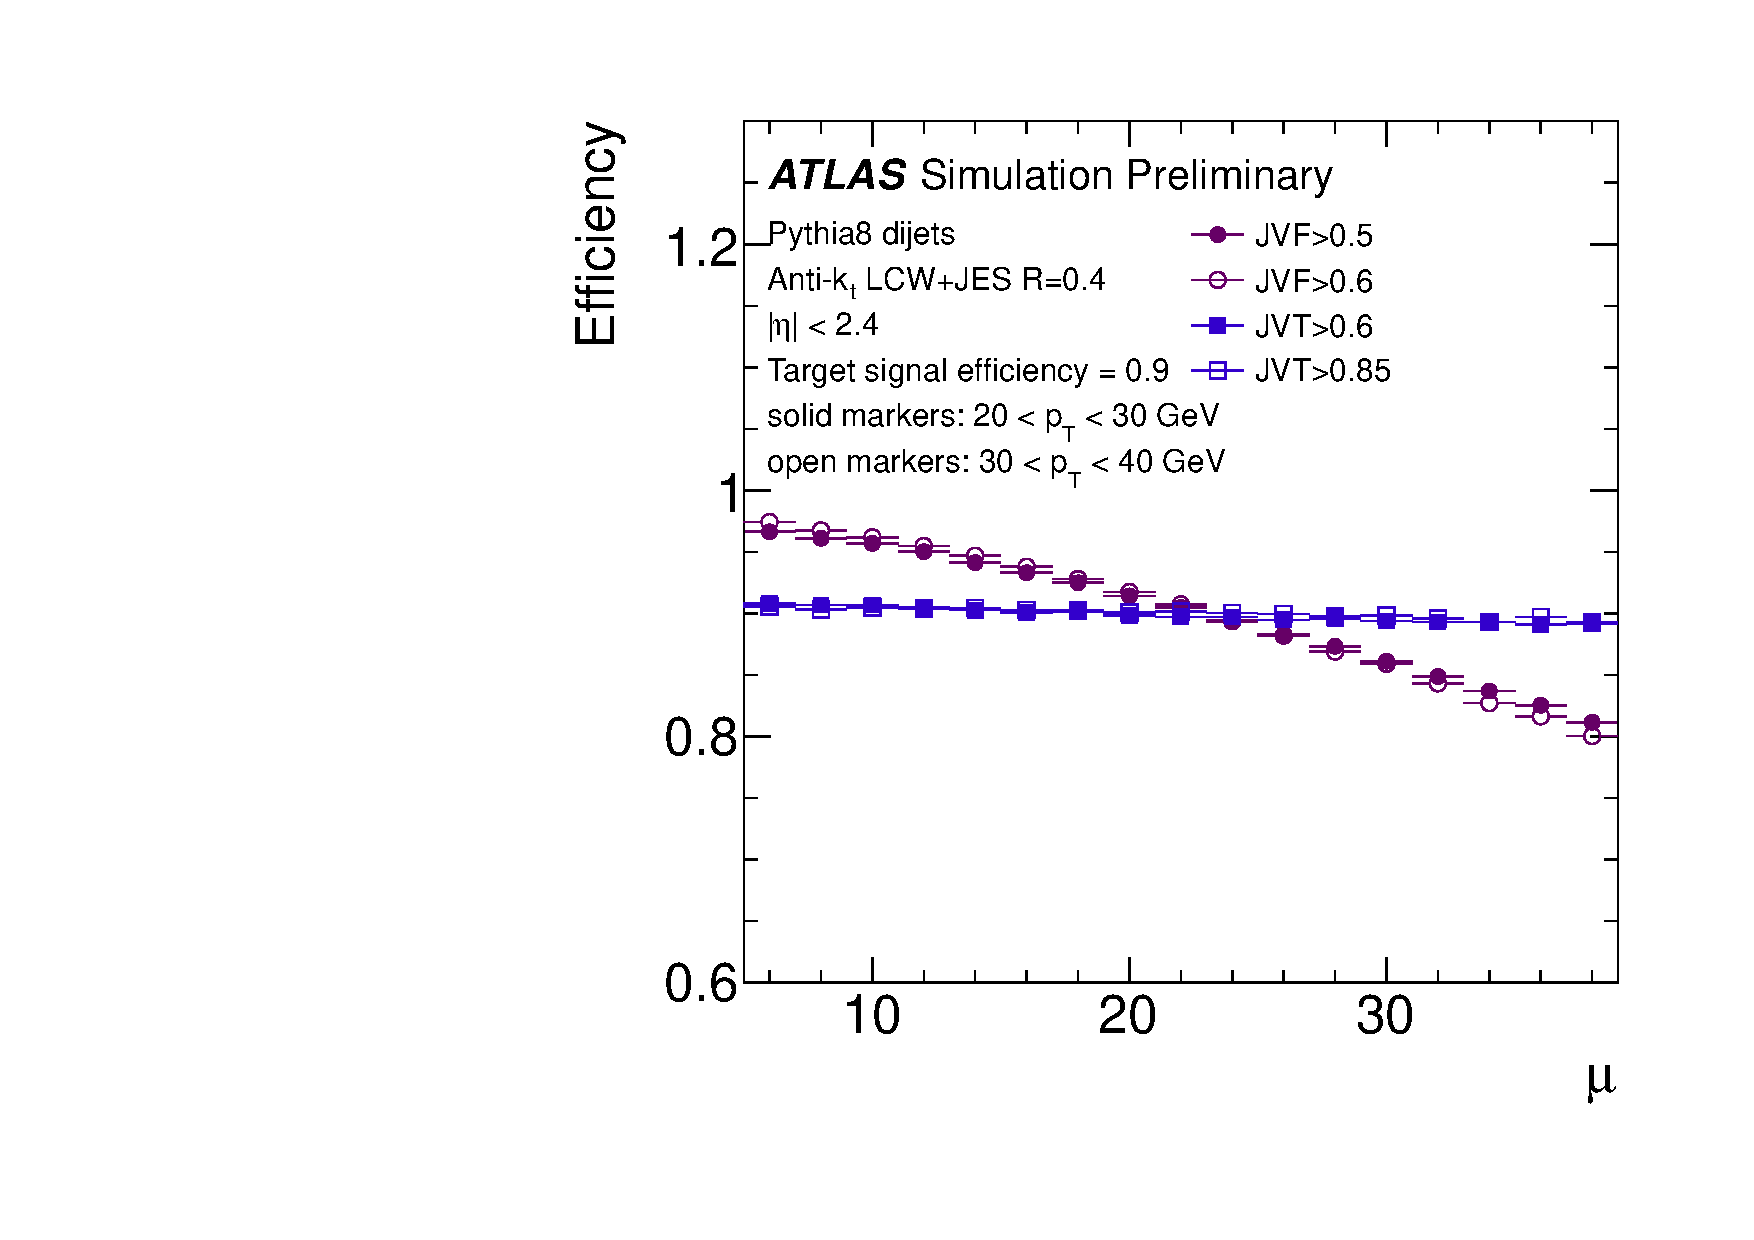
\includegraphics[width= 0.46\textwidth]{JVT_stability_eff90_mu}
  \label{fig:fig:JVT_stab_90_mu}
  }
  \subfigure[]{
  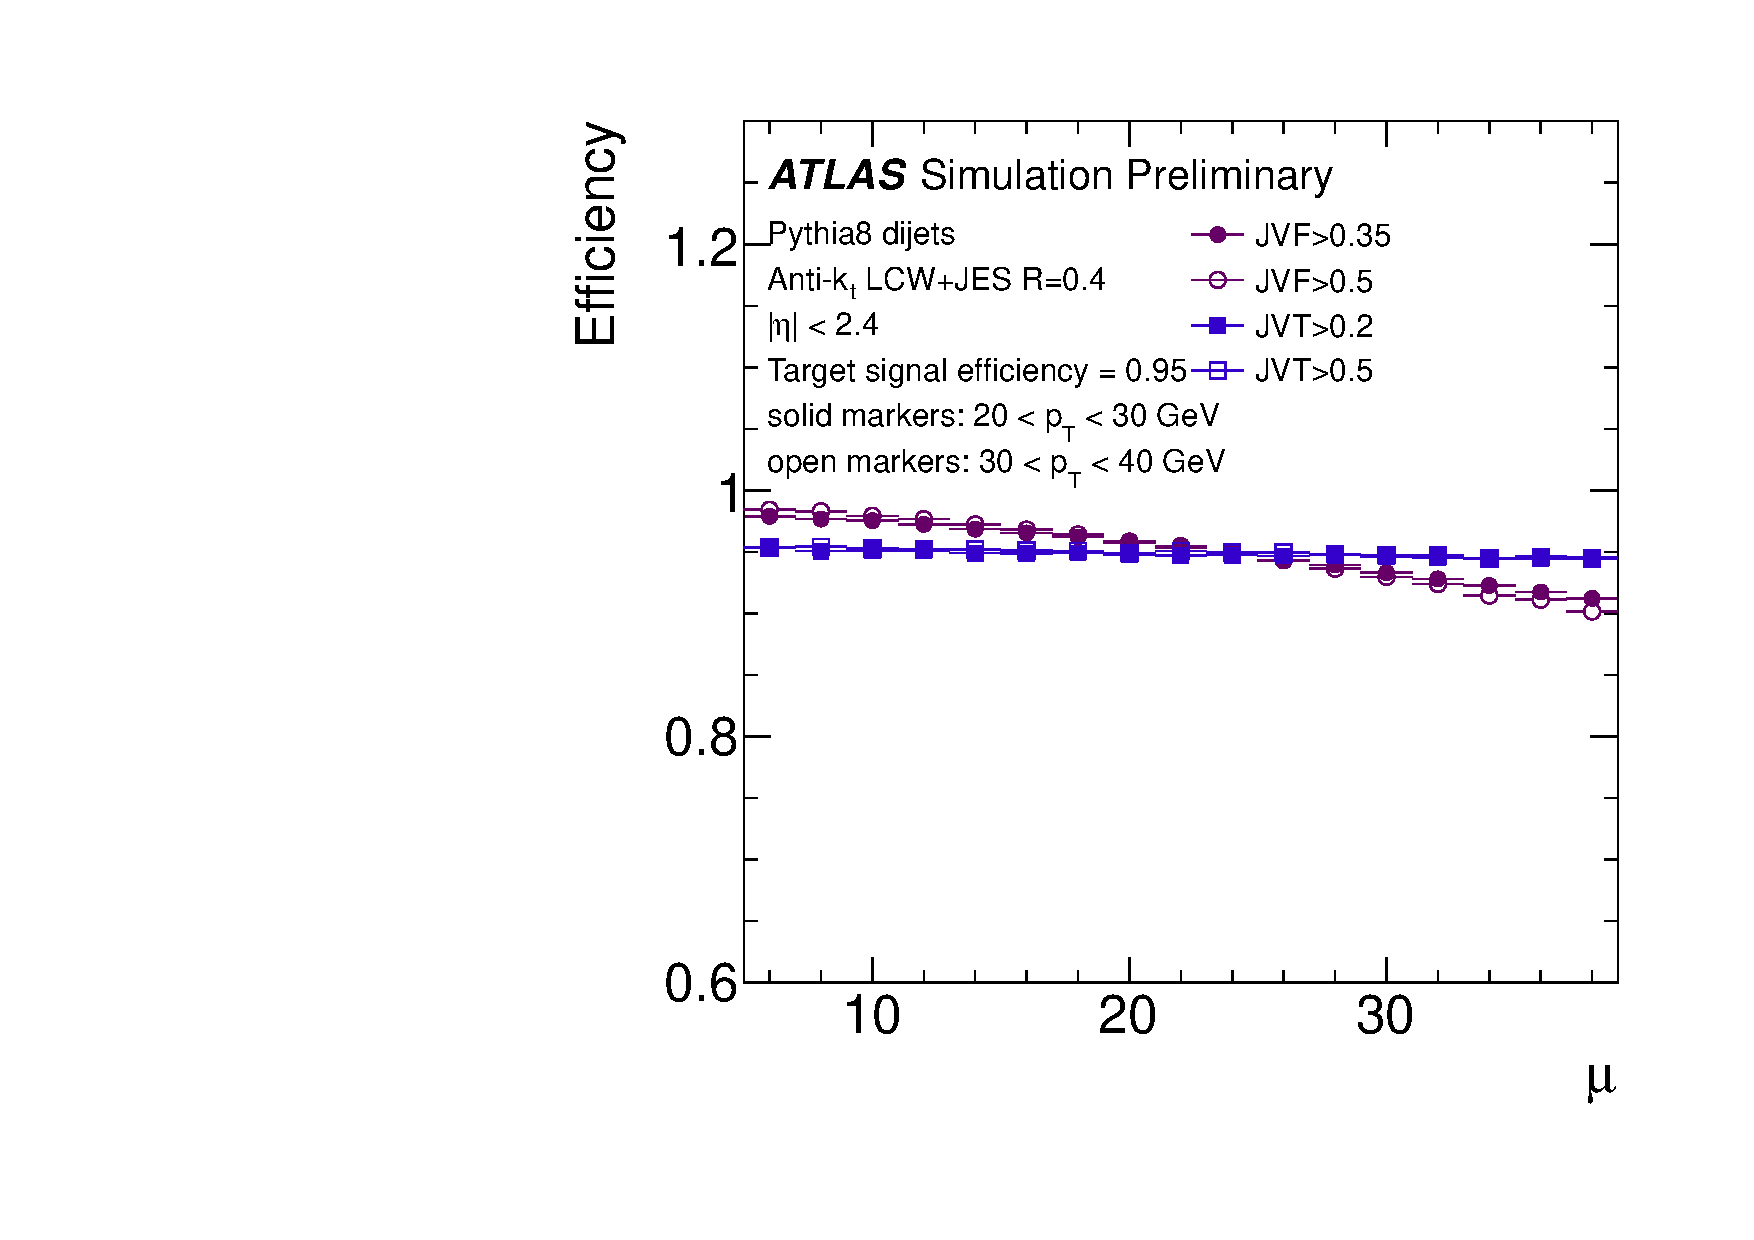
\includegraphics[width= 0.46\textwidth]{JVT_stability_eff95_mu}
  \label{fig:fig:JVT_stab_95_mu}
  }
  \caption{Dependence of the hard-scatter 
           jet efficiency for $20 < \pT < 30\GeV$ (solid markers) and $30 < \pT < 40\GeV$ (open markers) 
           jets as a function of the average number of interactions per bunch crossing $\mu$. 
           Fixed cuts of \JVT (blue) and \JVF (violet) are imposed such that the inclusive efficiency is $90\%$ (a) and $95\%$ (b).
           The cut values imposed on \JVT and \JVF, which depend on the \pT bin, are specified in the legend.}
  \label{fig:JVT_stab_mu}
\end{figure}
%------------------------


%-----------------------------------------------------------------------------------------------------------------------------
\subsection{Flavor dependence}
The difference in fragmentation and showering between light-quark and gluon initiated jets is expected to affect the shapes of \cJVF and \RpT and 
thus the performance of the \JVT based pileup jet suppression. 
The \cJVF- and \RpT-based discrimination between pileup and hard-scatter jets relies on 
the successful reconstruction and association of the hard-scatter tracks.
Light (uds)-quark initiated jets have on average a lower number of associated hard-scatter tracks but a slightly higher response~\cite{ATLAS-CONF-2012-138} and
both effects lead towards an increase in the number of jets with no associated tracks from the hard-scatter primary vertex with 
respect to gluon initiated jets. 

%---------------------
\begin{figure}[!htbp]
  \centering
  \subfigure[]{
  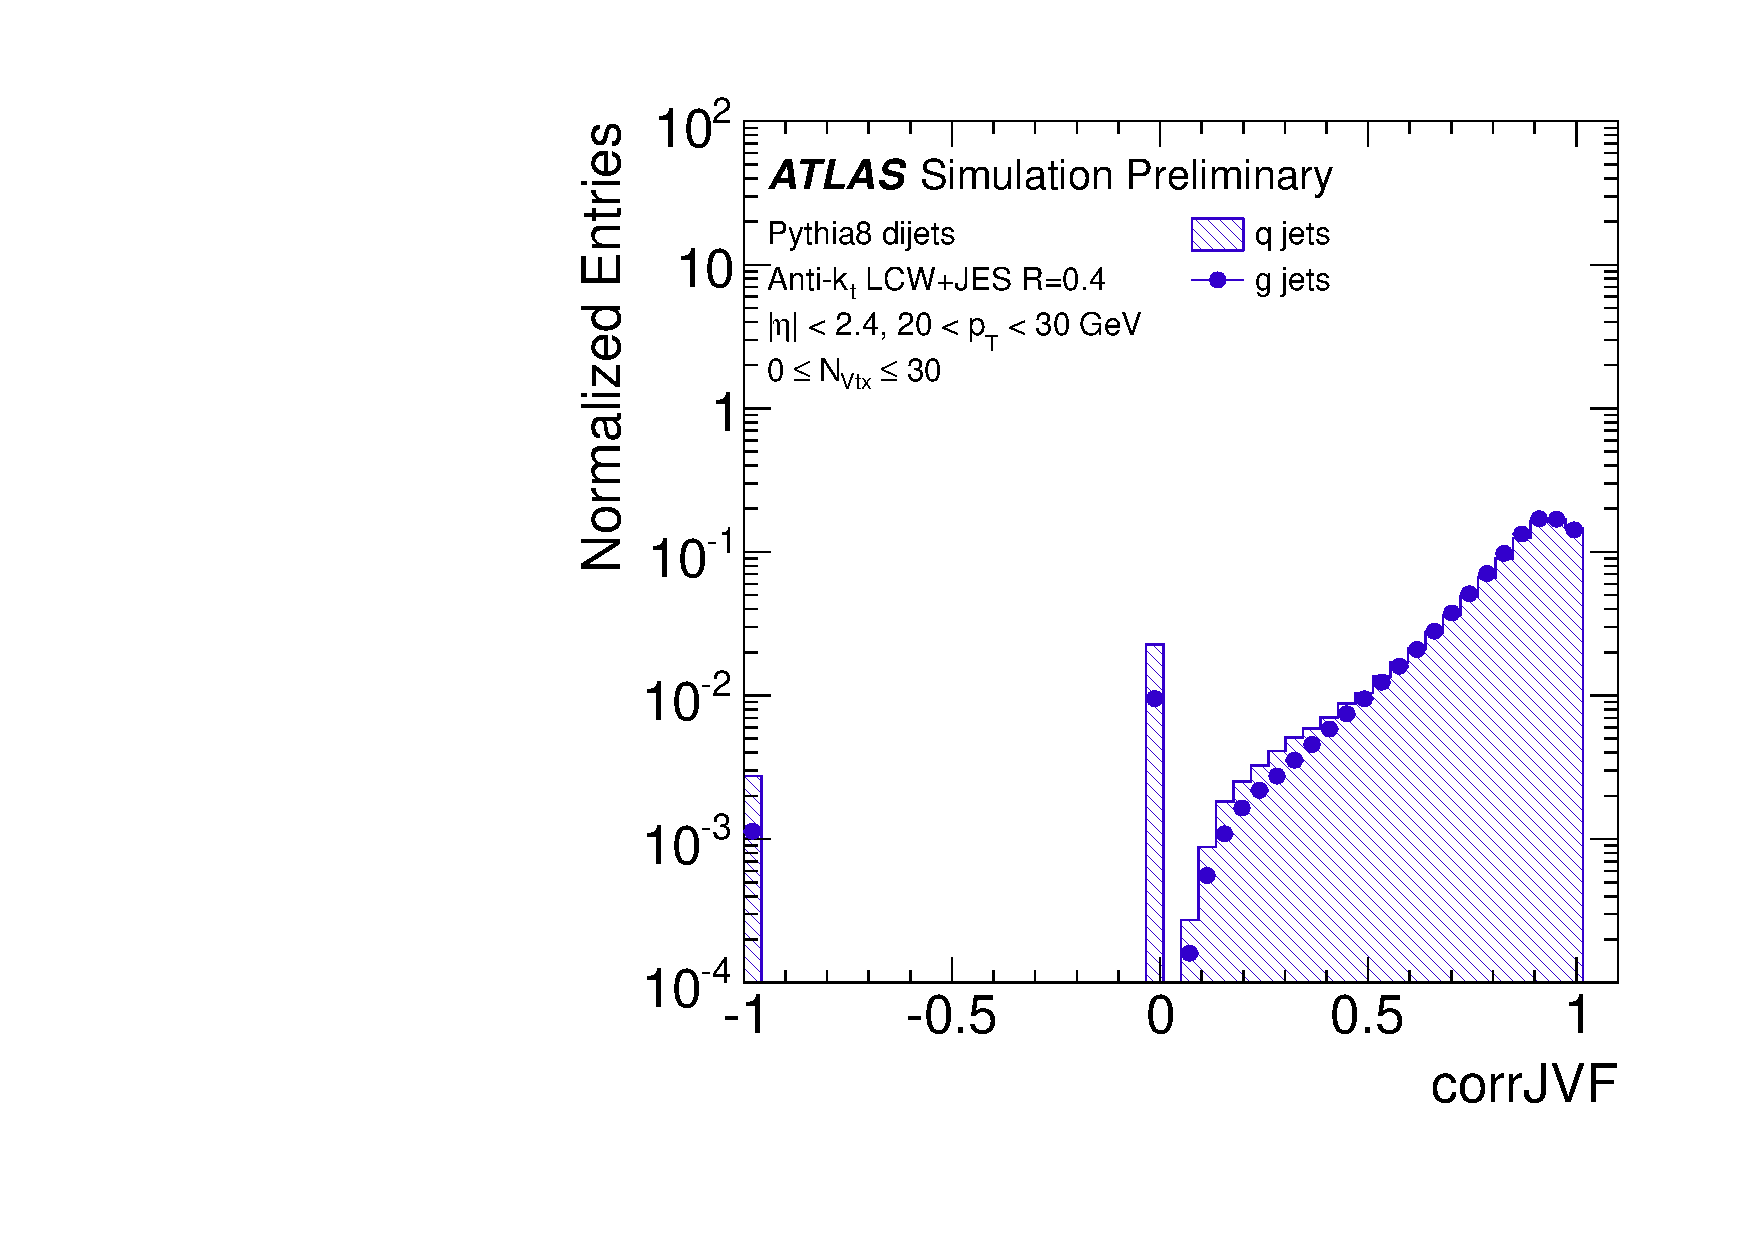
\includegraphics[width= 0.31\textwidth]{corrJVF_pt20to30_q_vs_g}
  \label{fig:corrJVF_flavor_dep_1}
  }
  \subfigure[]{
      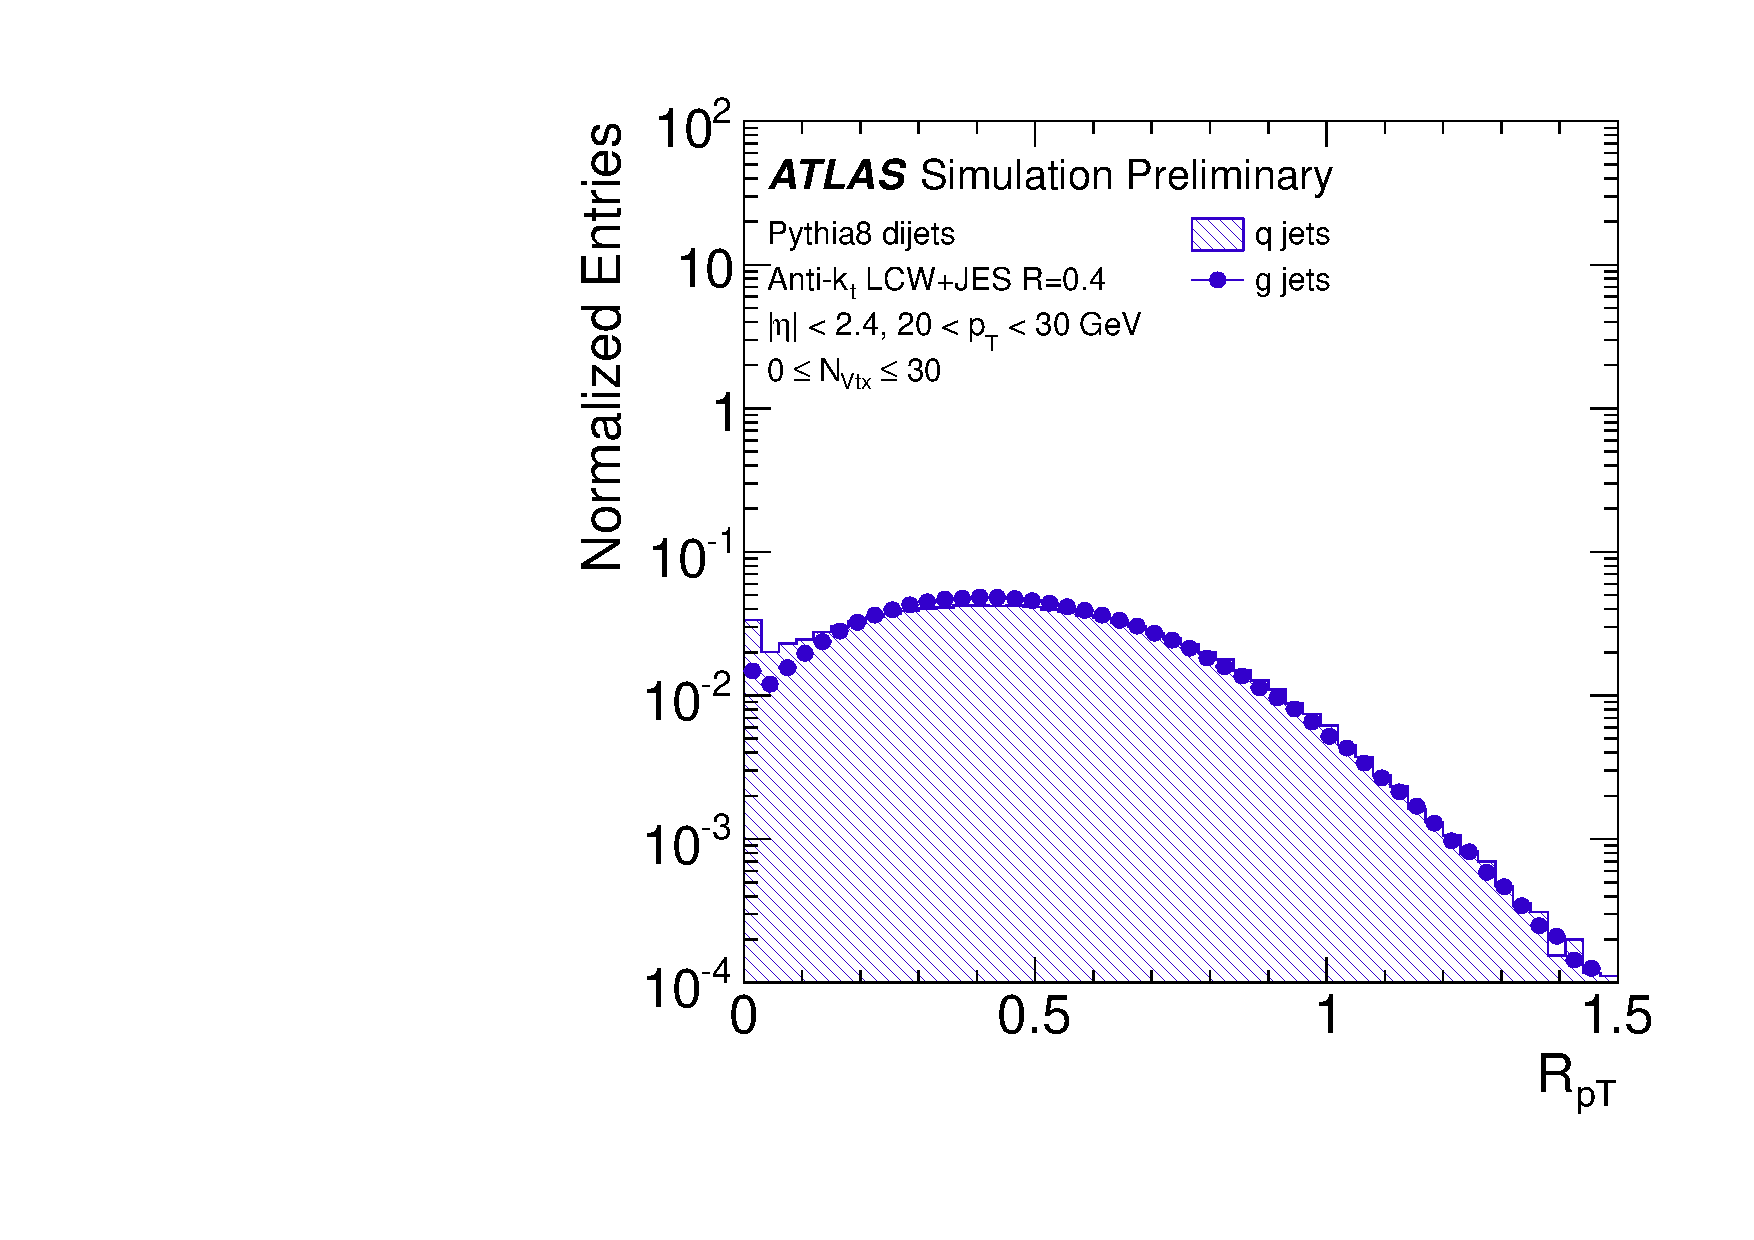
\includegraphics[width= 0.31\textwidth]{RpT_pt20to30_q_vs_g}
  \label{fig:RpT_flavor_dep_2}
  }
  \subfigure[]{
      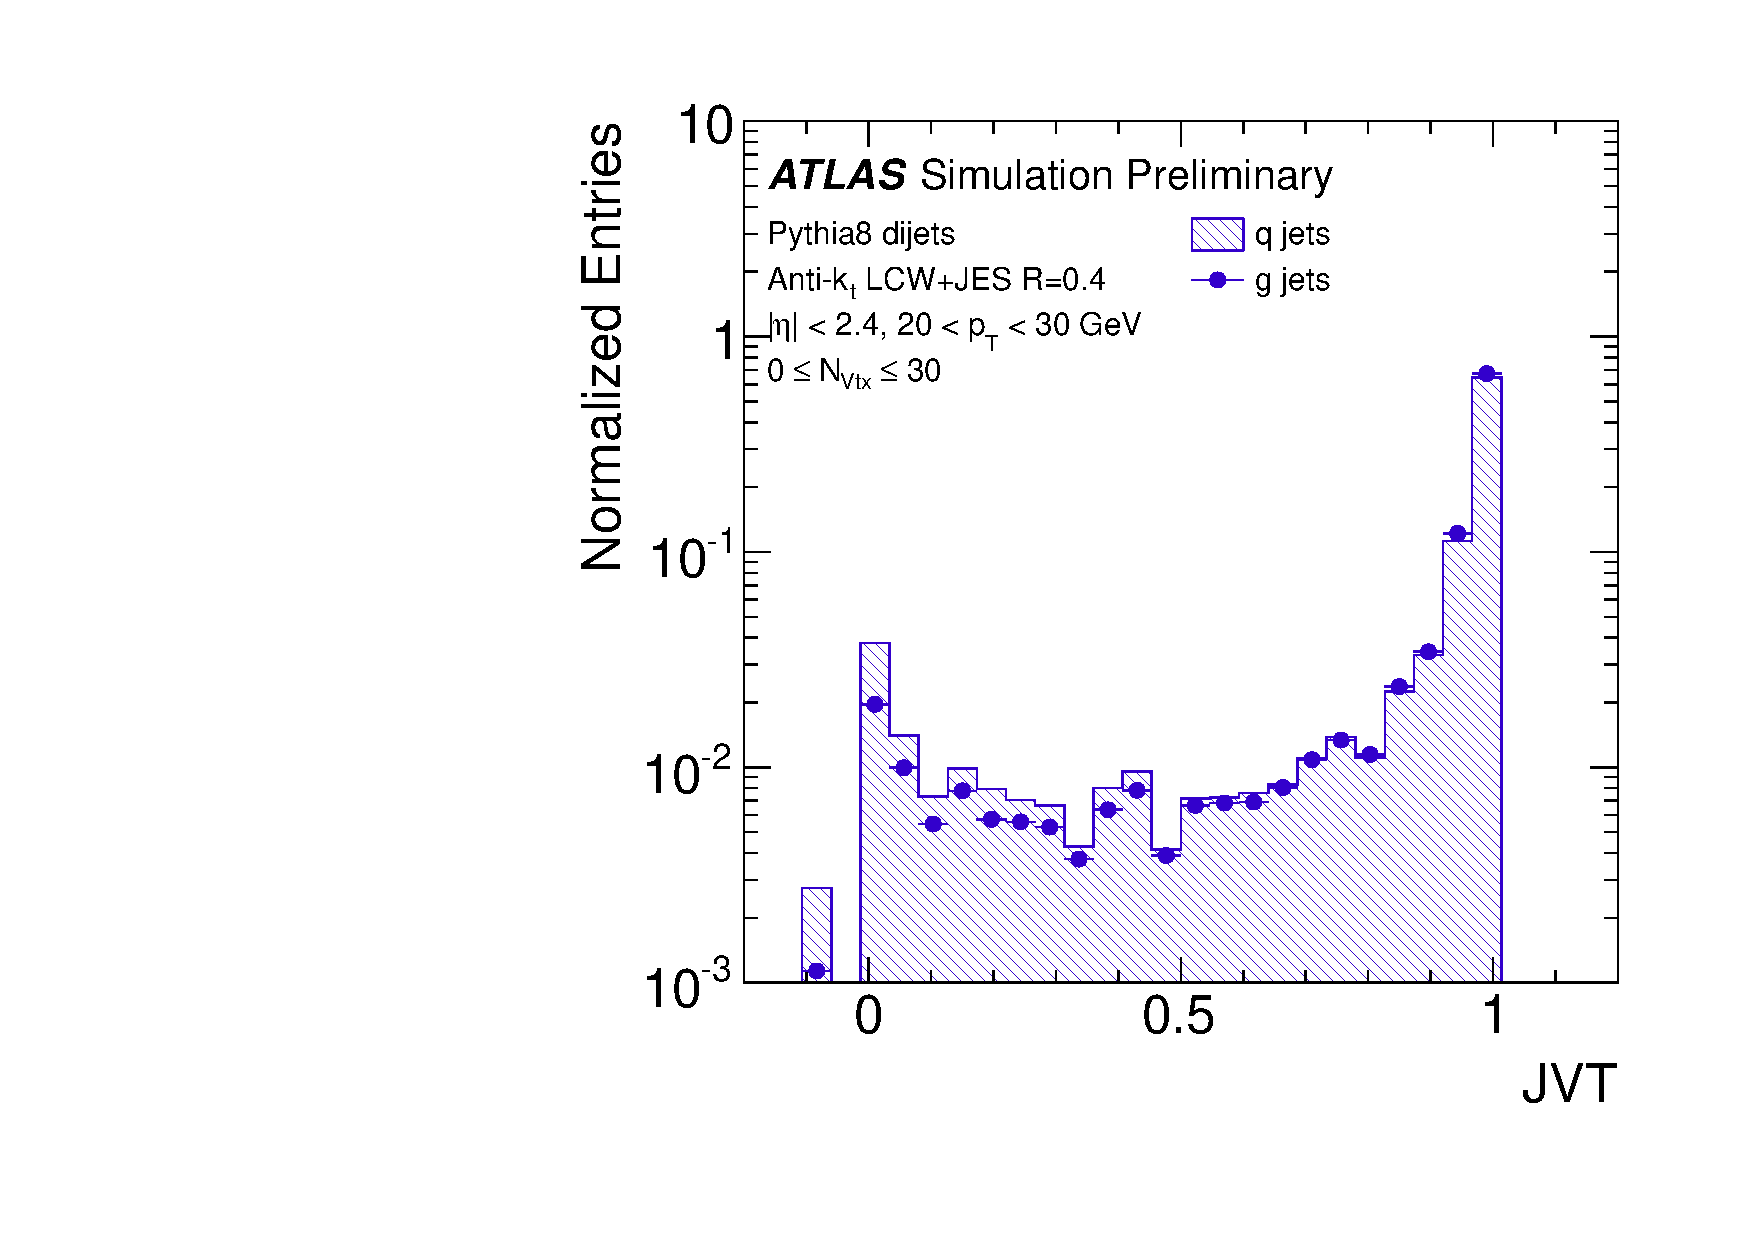
\includegraphics[width= 0.31\textwidth]{JVT_pt20to30_q_vs_g}
  \label{fig:JVT_flavor_dep_3}
  }
  \caption{The distributions of \cJVF (a), \RpT (b) and \JVT (c) for light-quark and gluon initiated hard-scatter jets.}
  \label{fig:flavor_dep}
\end{figure}
%------------------------
In \Figref{fig:flavor_dep} we show the \cJVF, \RpT and \JVT distributions for light-quark and gluon initiated hard-scatter jets with 
$20<\pT<30\GeV$. Using a leading order notion of jet flavor, the partonic flavor labeling refers to the highest energy parton within a narrow cone
of $\Delta R<0.3$ 
around the jet axis.
The distributions for light-quark initiated
jets have more entries at low \cJVF, \RpT and \JVT values and consequently a worse separation from pileup jets. 
Most notably, about twice as many light-quark jets have no associated tracks 
from the hard-scatter primary vertex, thus $\cJVF=\JVT=0$. 

%---------------------
\begin{figure}[!htbp]
  \centering
  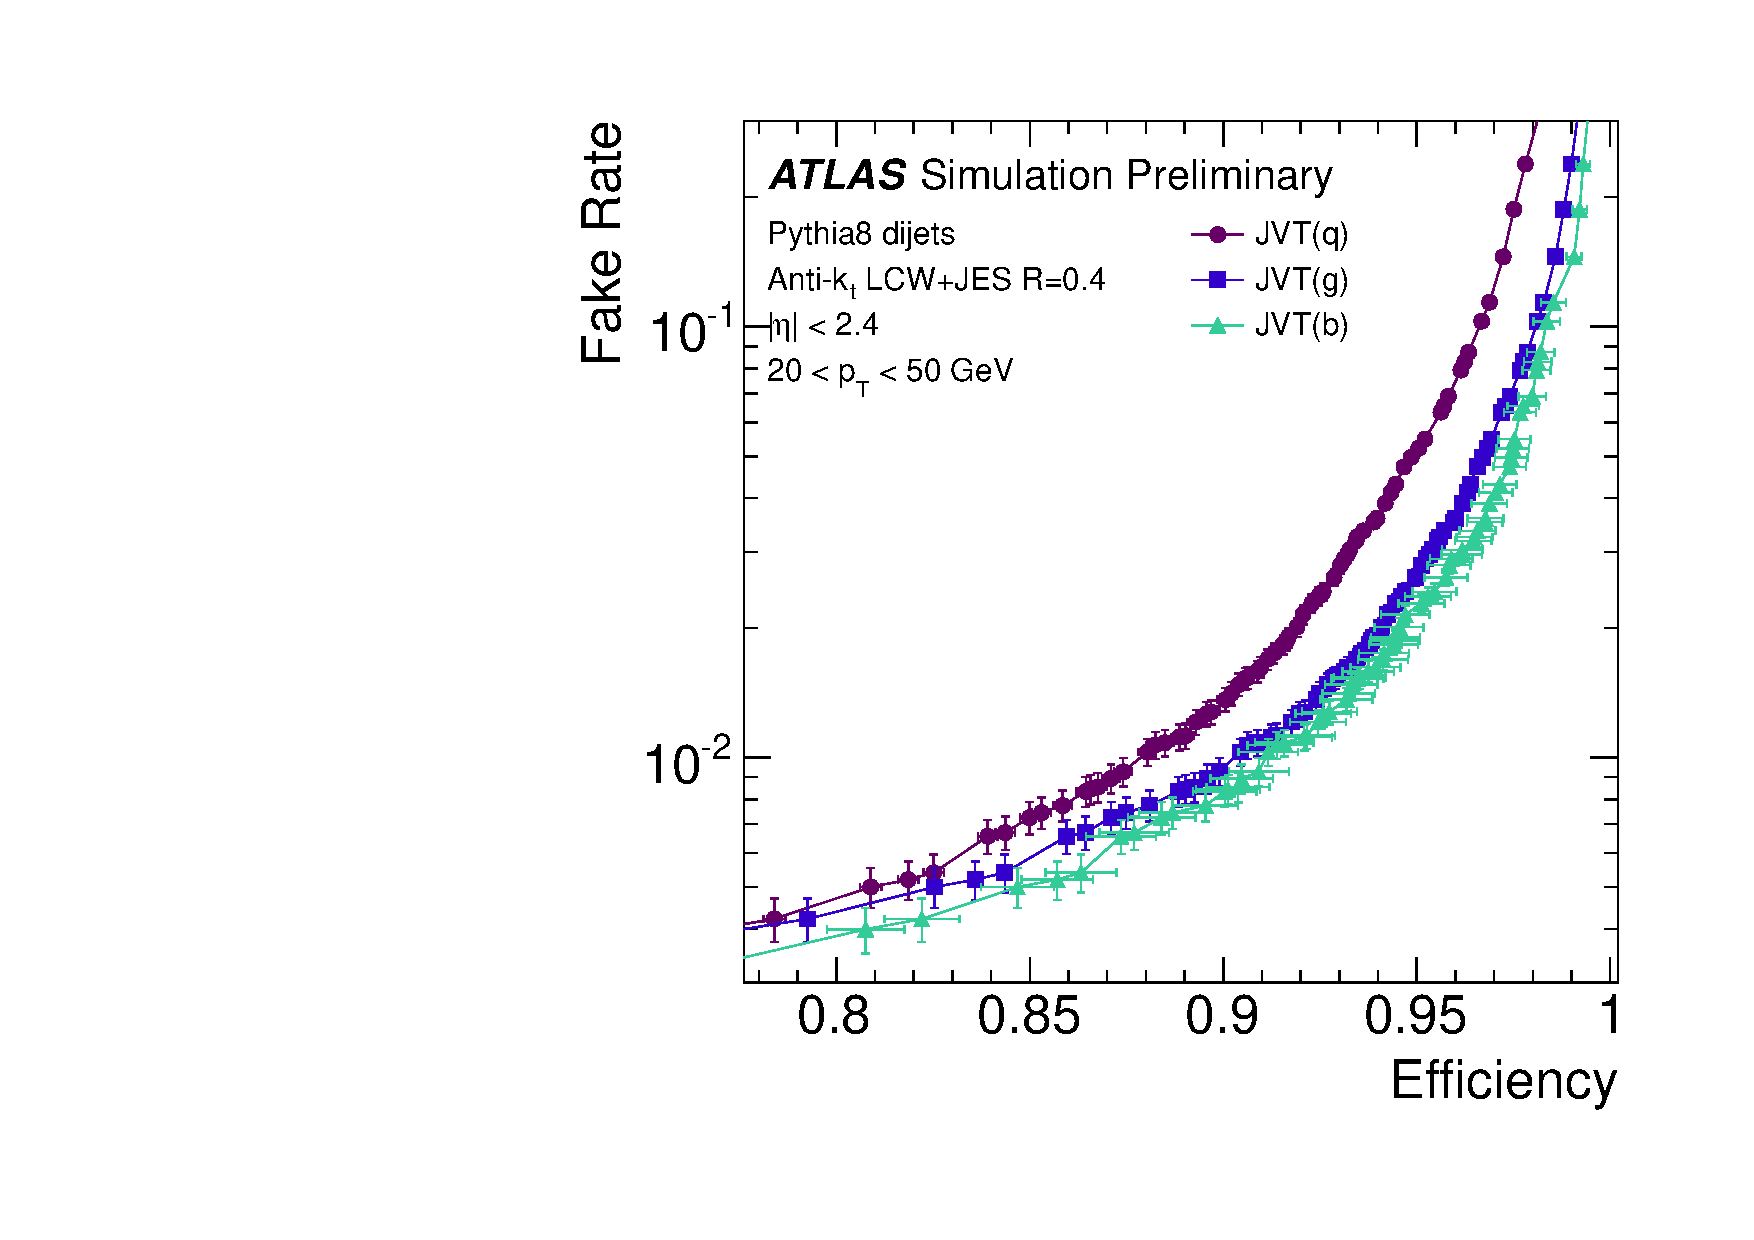
\includegraphics[width= 0.46\textwidth]{ROC_JVT_q_vs_g_vs_b}
  \caption{The fake rate from pileup jets versus hard-scatter jet efficiency curves for \JVT separating light-quark, gluon and b-quark initiated jets.}
  \label{fig:ROC_q_vs_g_vs_b}
\end{figure}
%------------------------
Figure~\ref{fig:ROC_q_vs_g_vs_b} shows the efficiency \vs fake-rate curve for \JVT for light-quark, gluon and b-quark initiated jets. 
As expected from Figure~\ref{fig:flavor_dep}, the performance is worse for light-quark initiated jets. The pileup \vs hard-scatter jet discrimination
is best performing for b-quark initiated hard-scatter jets, profiting from the optimized track-to-vertex association as described in Section~\ref{sec:OS}.
It was found that the efficiency \vs fake-rate curve for c-quark labeled jets is marginally worse than the one of gluon jets. 
When imposing minimal \cJVF, \RpT or \JVT criteria, the hard-scatter jet efficiencies are lower for light-quark initiated than for gluon initiated jets.

The stability 
of the hard-scatter efficiencies as a function of \NPV is found to be independent of the flavor of the jet initiating parton. 


%----------------------------------------------------------------------
\section{Validation of the modeling in data}
\label{sec:JVTvalidation}
%--------------------------
%---------------------
\begin{figure}[!htbp]
  \centering
  \subfigure[]{
      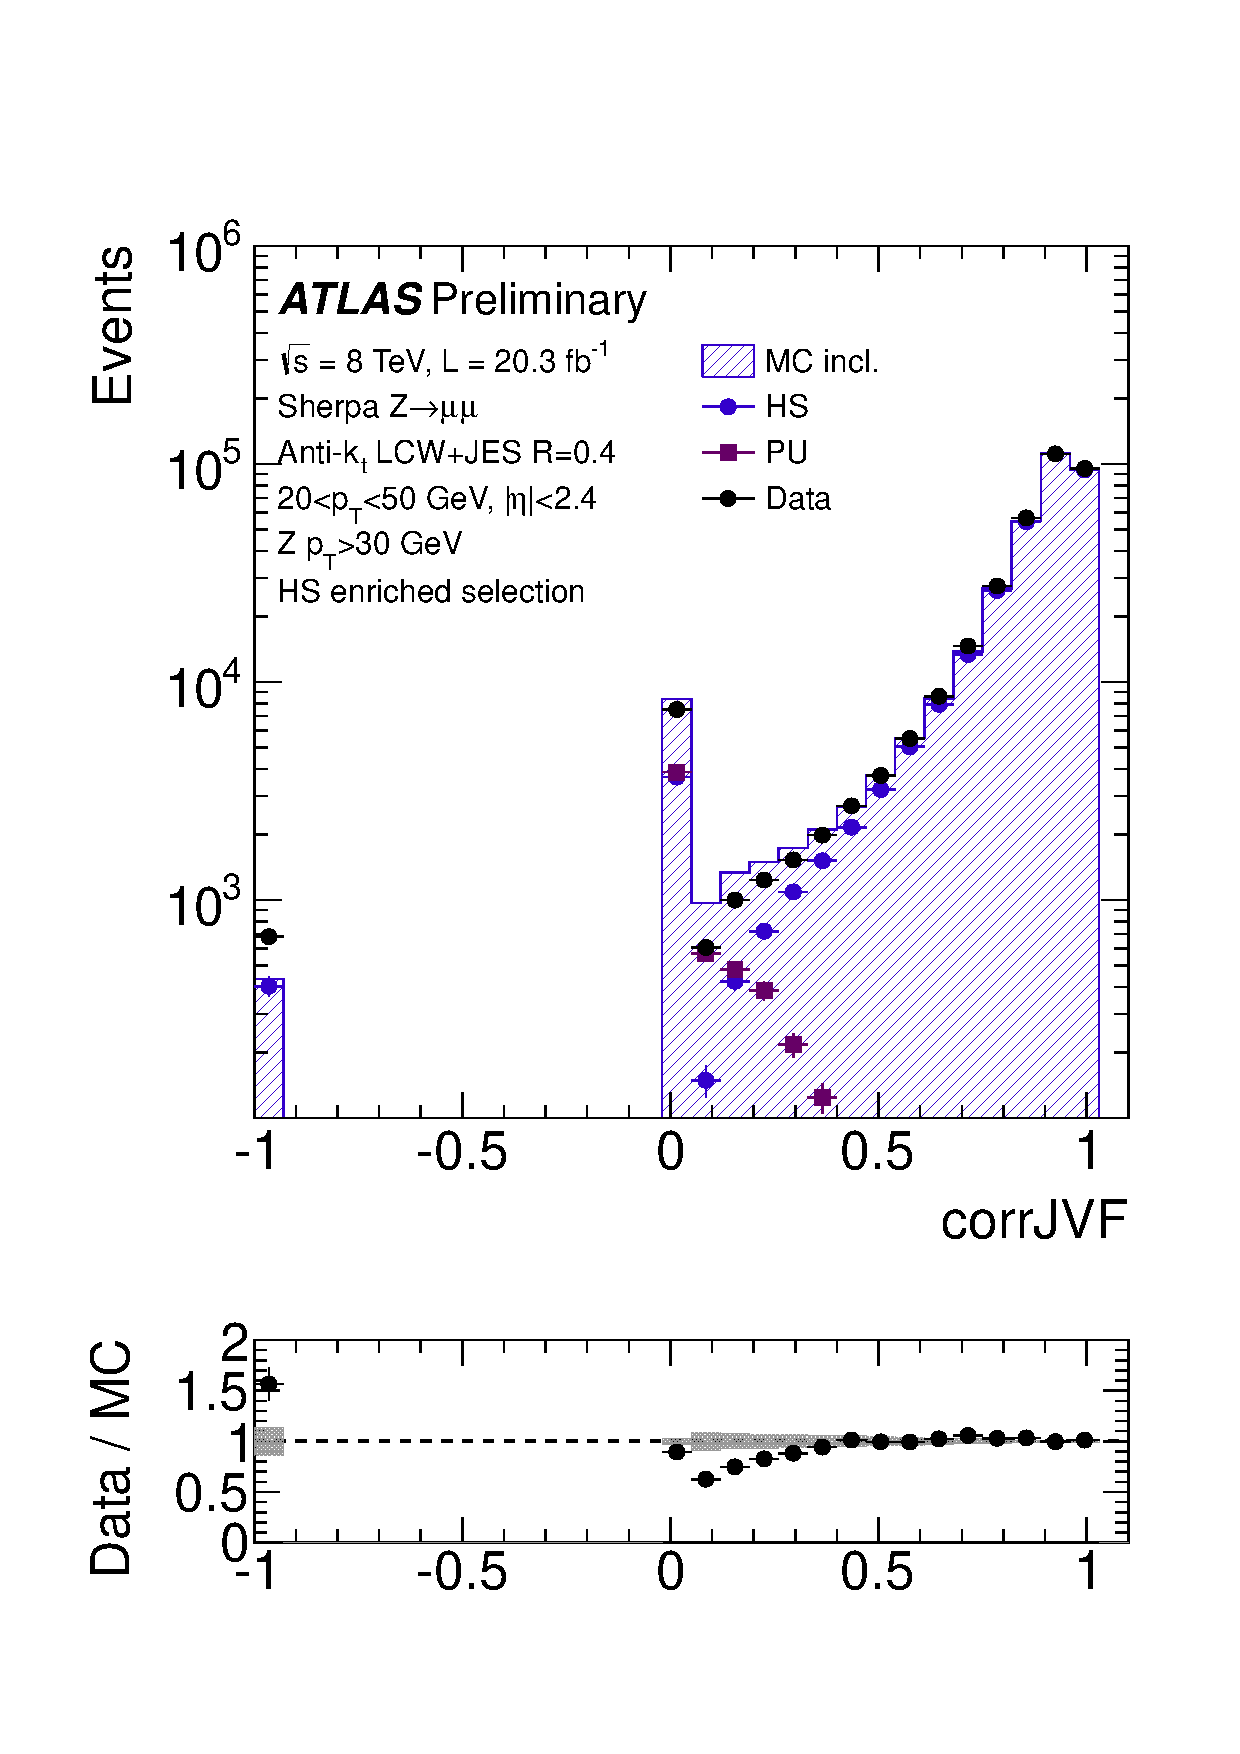
\includegraphics[width= 0.31\textwidth]{corrJVF_HSenriched}
      \label{fig:Zmumu_HS_corrJVF}
  }
  \subfigure[]{
      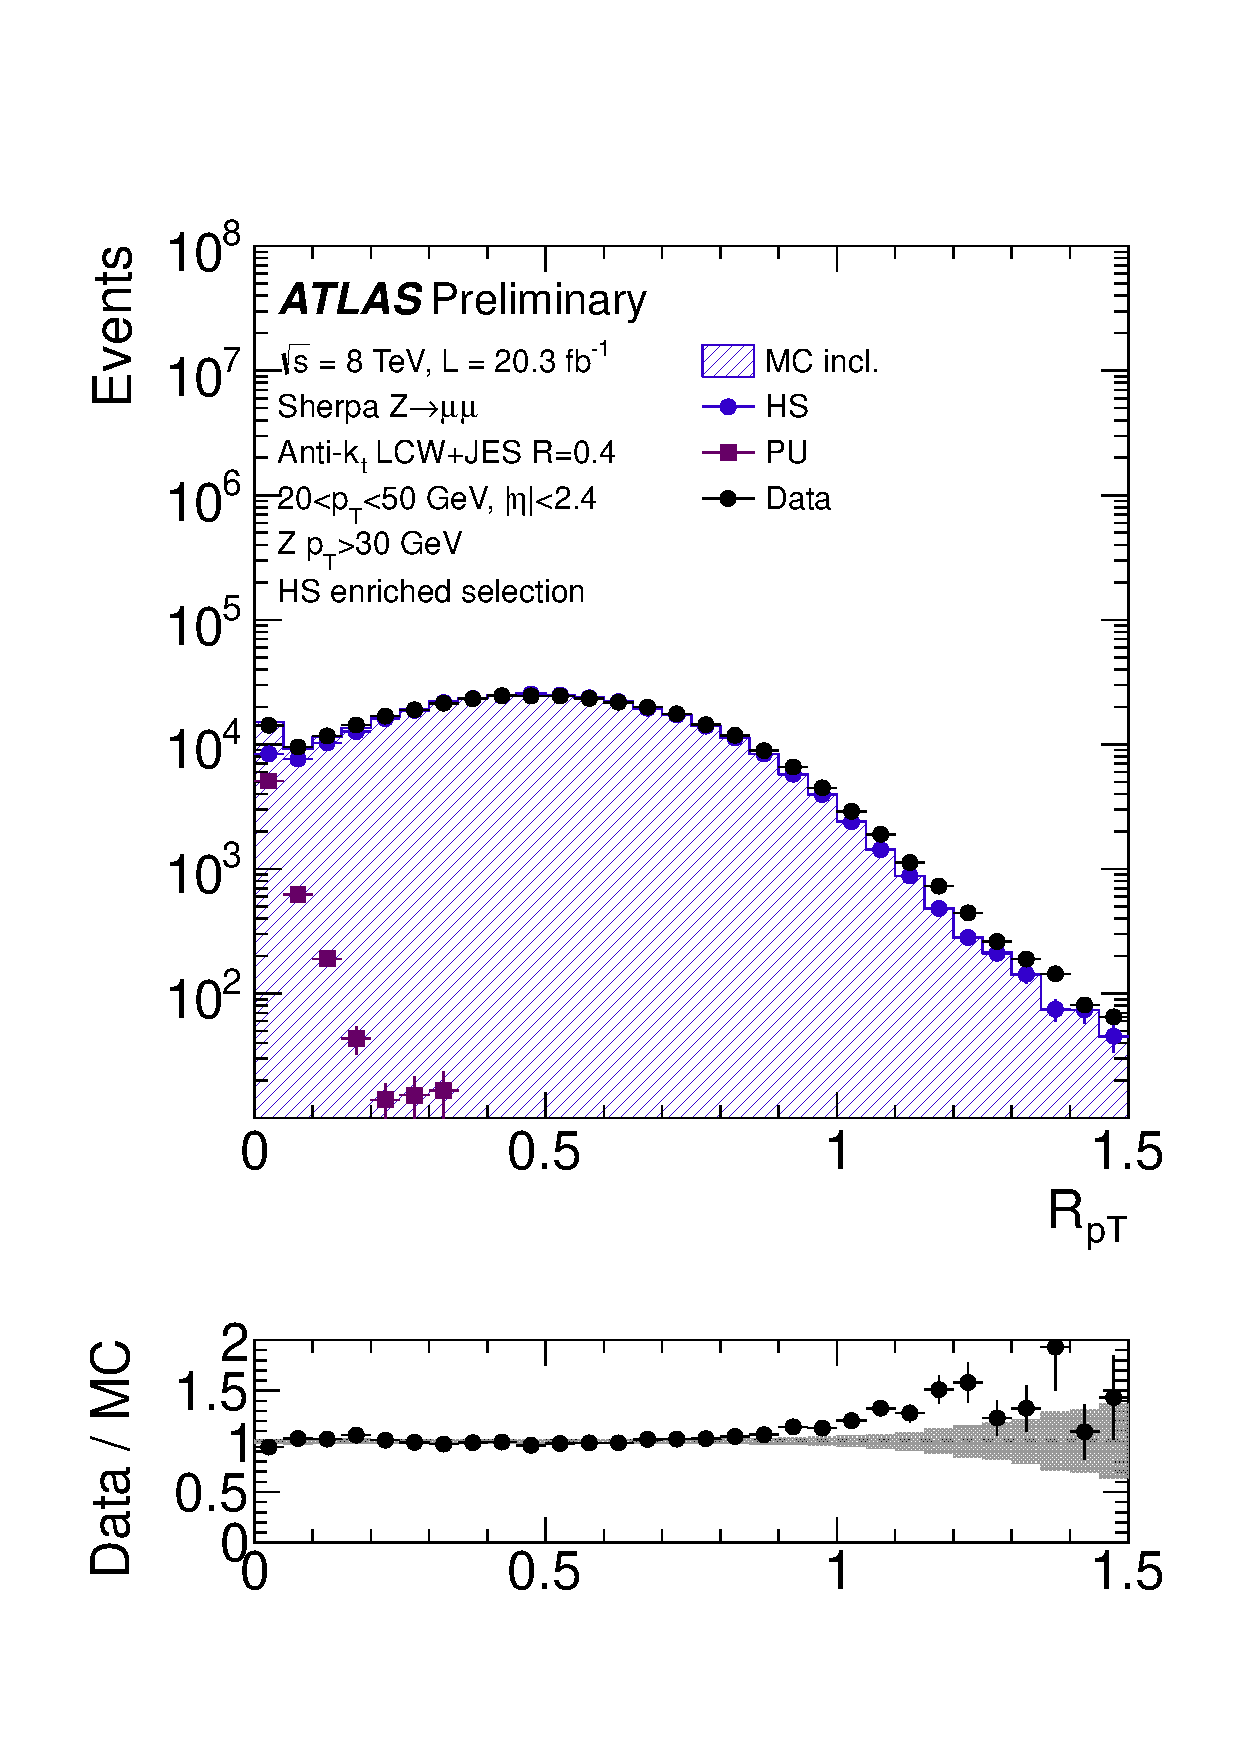
\includegraphics[width= 0.31\textwidth]{RpT_HSenriched}
  \label{fig:Zmumu_HS_RpT}
  }
  \subfigure[]{
      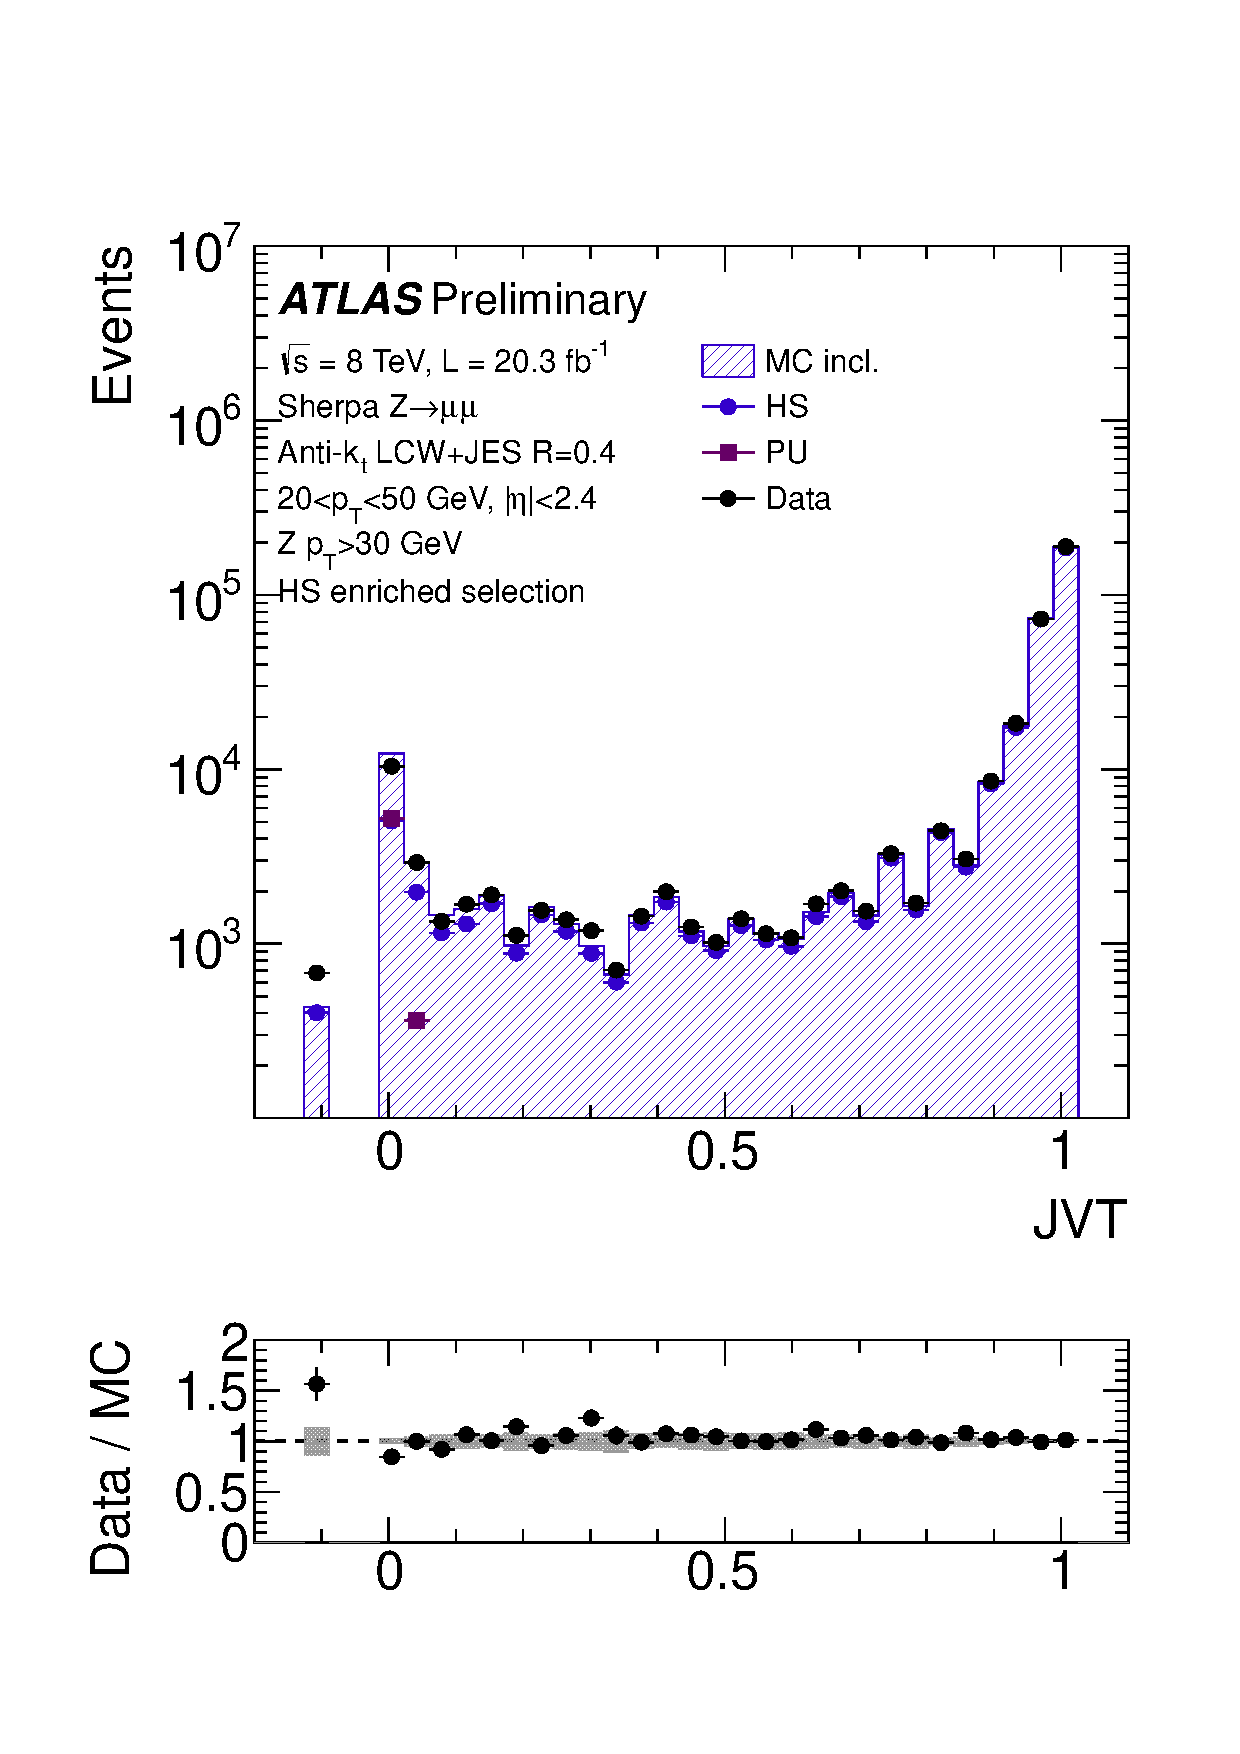
\includegraphics[width= 0.31\textwidth]{JVT_HSenriched}
  \label{fig:Zmumu_HS_JVT}
  }
  \caption{Comparison between data and simulation for \cJVF (a), \RpT (b) and \JVT (c) in a hard-scatter enriched selection of jets in $\Zboson(\to\mu\mu)$+jets events,
      where a $|\Delta \phi(\Zboson, {\rm jet})|>2.6$ requirement is imposed between the leading jet and the \Zboson boson.
  The blue shaded histogram representing the inclusive simulation is subdivided in its hard-scatter jet and pileup jet contributions
  using blue and magenta markers respectively.  
  The gray band in the ratio plot represents the statistical uncertainty in the simulation. The bin-by-bin variations in the \JVT distribution are due to the discrete (rather than continuous) nature of the variable.}
  \label{fig:Zmumu_HS}
\end{figure}
\begin{figure}[!htbp]
  \centering
  \subfigure[]{
      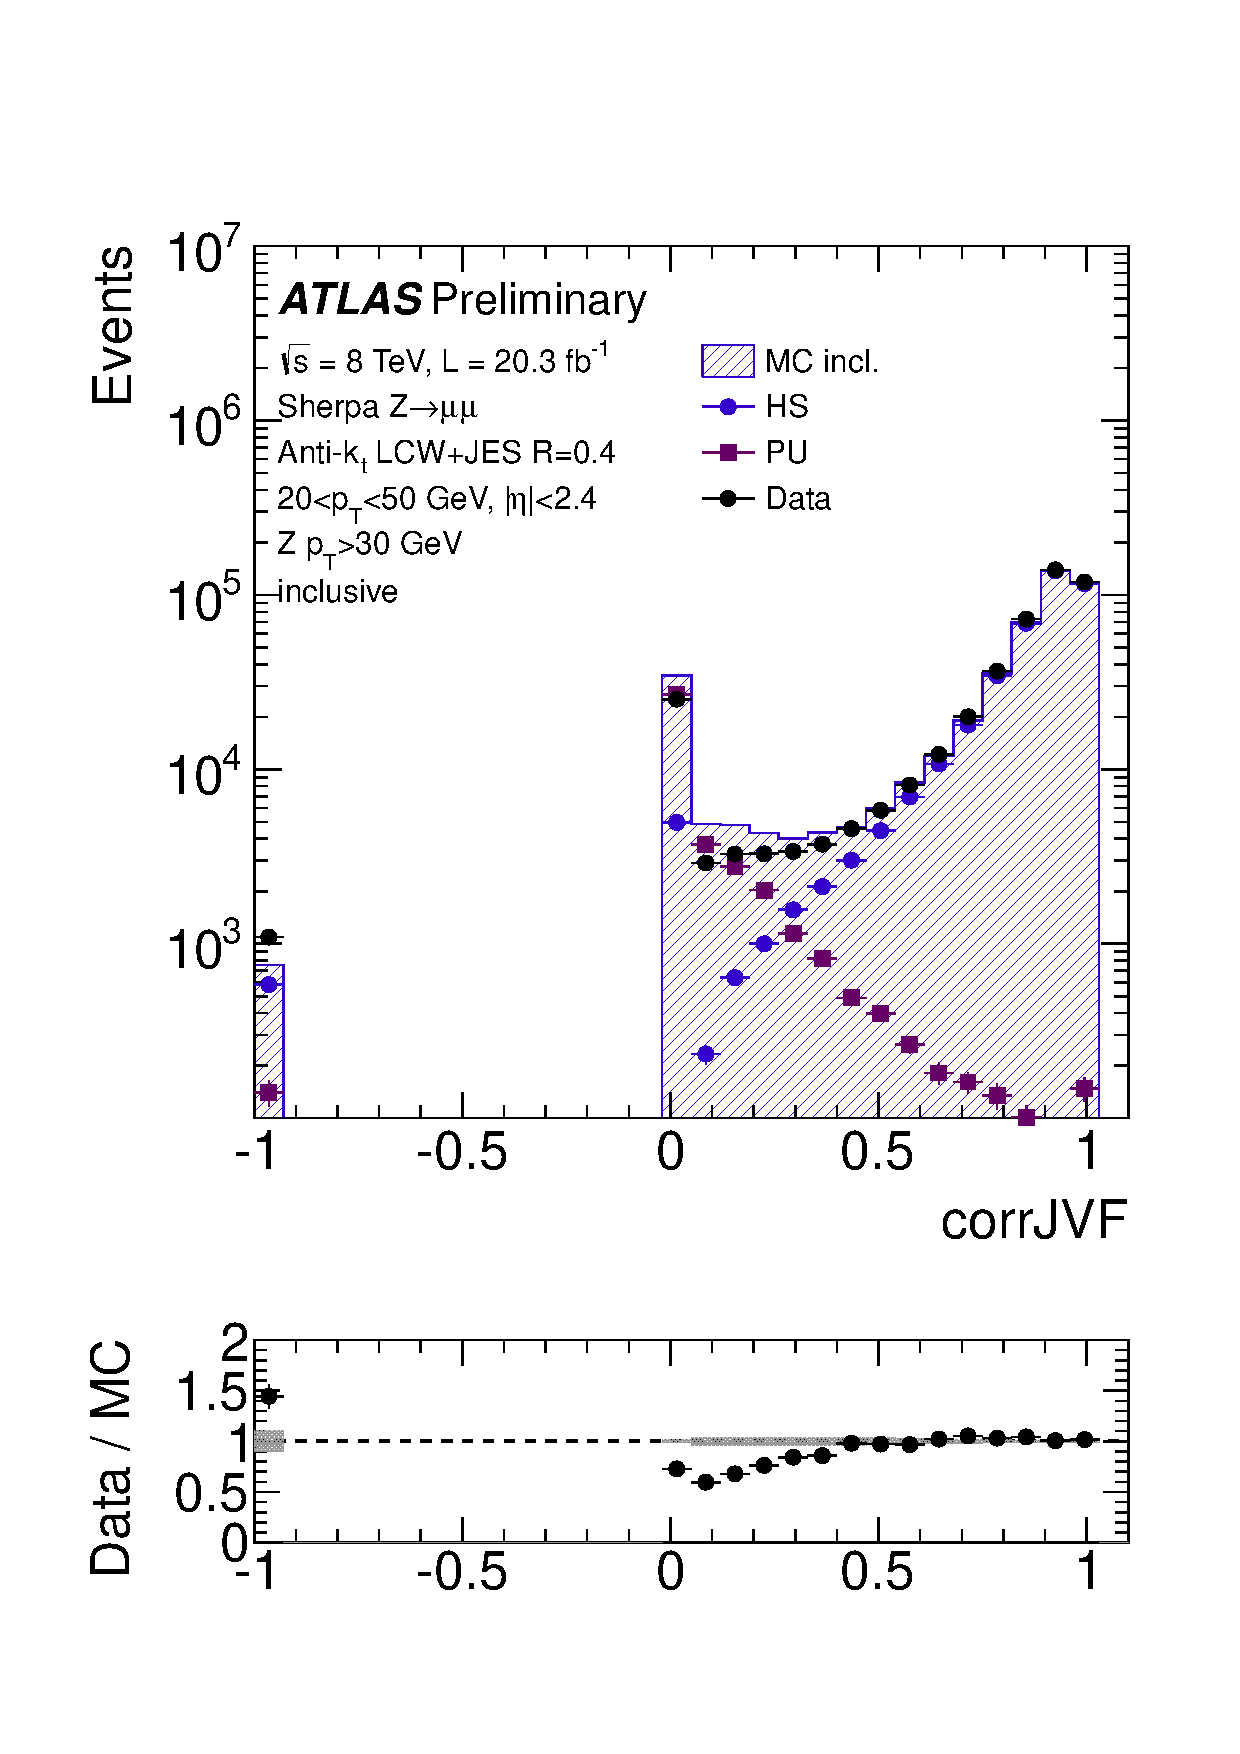
\includegraphics[width= 0.31\textwidth]{corrJVF_Zmumu_inclusive}
      \label{fig:Zmumu_incl_corrJVF}
  }
  \subfigure[]{
      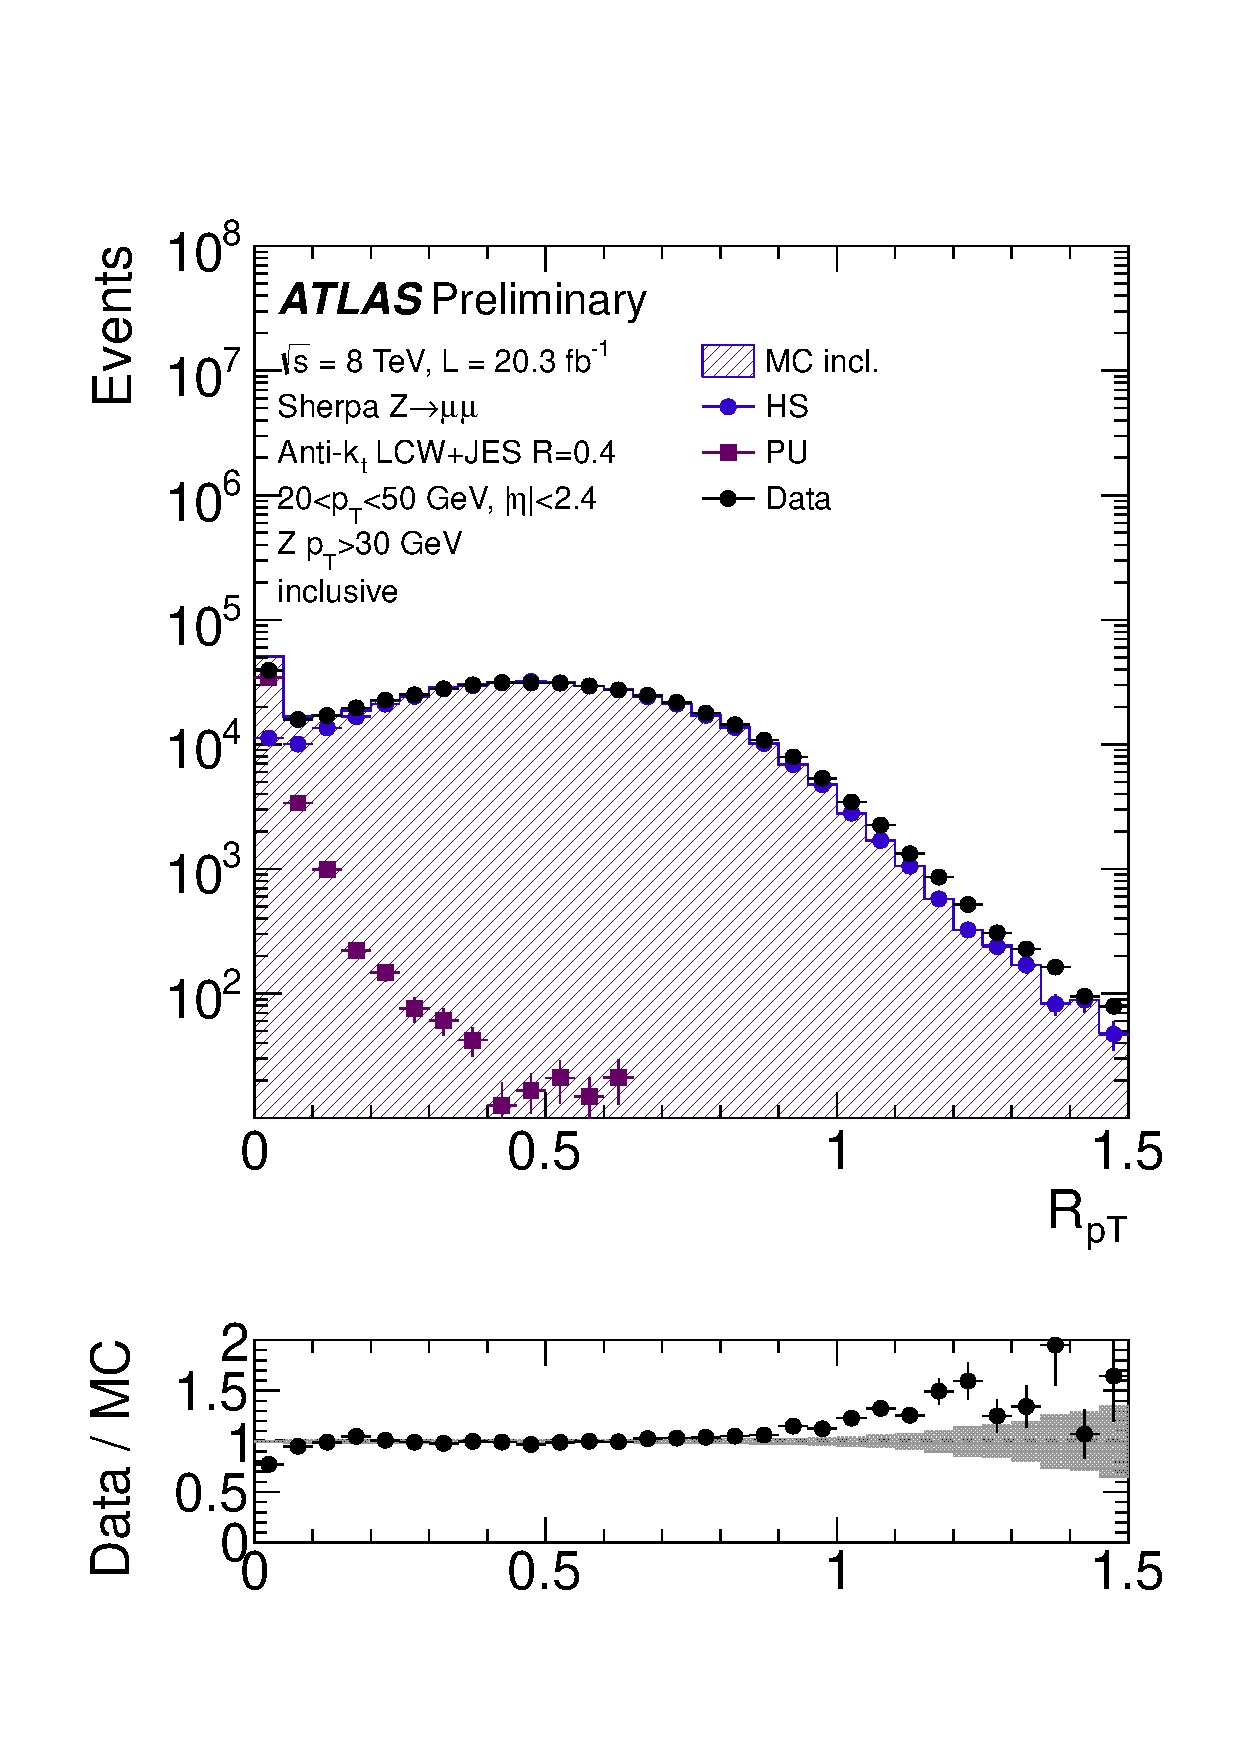
\includegraphics[width= 0.31\textwidth]{RpT_Zmumu_inclusive}
  \label{fig:Zmumu_incl_RpT}
  }
  \subfigure[]{
      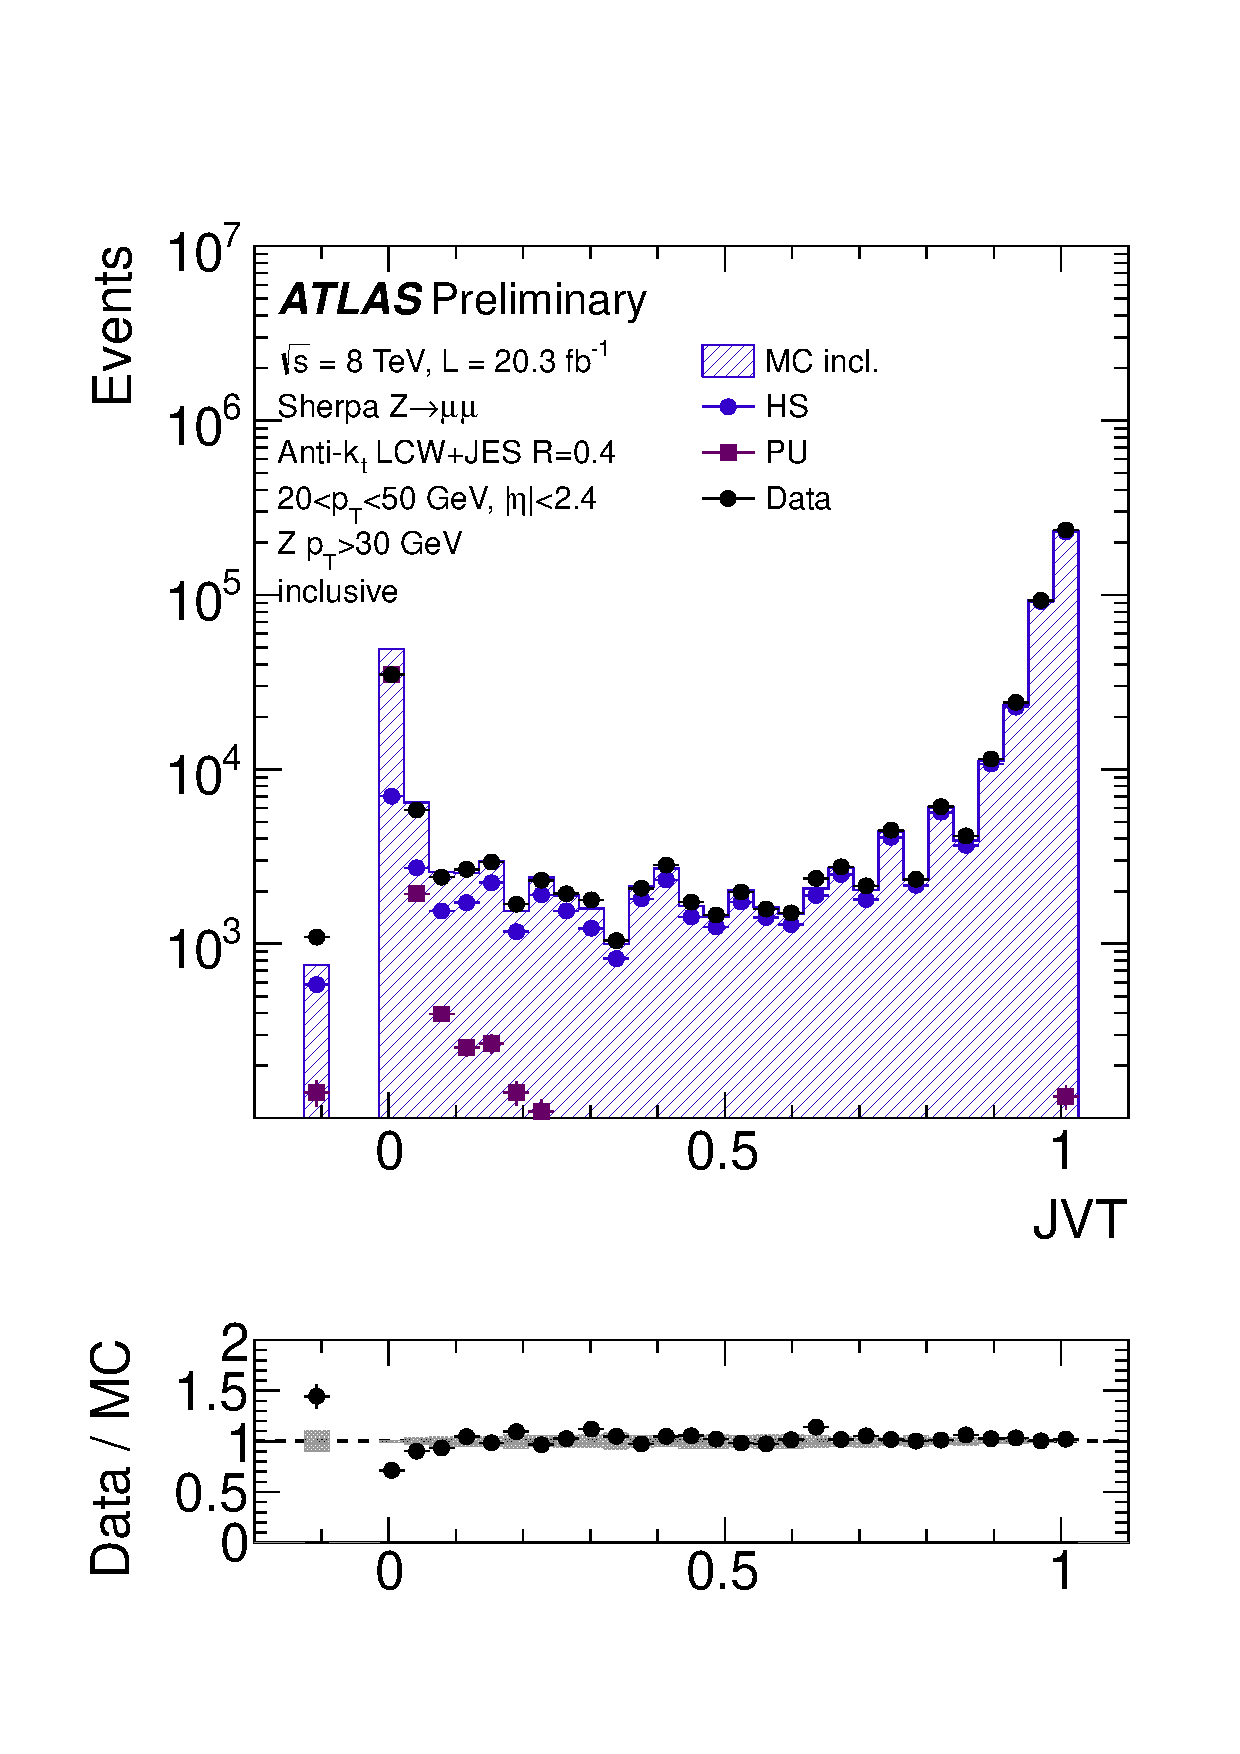
\includegraphics[width= 0.31\textwidth]{JVT_Zmumu_inclusive}
  \label{fig:Zmumu_incl_JVT}
  }
  \caption{\cJVF (a), \RpT (b) and \JVT (c) distributions for the leading jet with $20<\pT<50\GeV$ and $|\eta|<2.4$ in $\Zboson(\to\mu\mu)$+jets events, where the $|\Delta \phi(\Zboson, {\rm jet})|$
      requirement from Figure~\ref{fig:Zmumu_HS} is omitted.
  The blue shaded histogram representing the inclusive simulation is subdivided in its hard-scatter jet and pileup jet contributions
  using blue and magenta markers. 
  %The simulation is scaled to match the data in the hard-scatter dominated region. 
  The gray band in the ratio plot represents the statistical uncertainty in the simulation. The bin-by-bin variations in the \JVT distribution are due to the discrete (rather than continuous) nature of the variable.
%  It is seen that the pileup jet dominated bins $(\cJVF\in [0,0.3], \RpT<0.1, \JVT <0.05)$ 
%  are overestimated in the simulation by about 20\%.
  }
  \label{fig:Zmumu_incl}
\end{figure}
%------------------------
\subsection{Validation in $\Zboson(\to\mu\mu)$+jets events}
The modeling of  \RpT, \cJVF and \JVT can be validated with data using a sample of $\Zboson(\to\mu\mu)$ candidate  events where kinematic selection criteria
can be used to select either hard-scatter or pileup jets. In simulation, the non-\Zboson-boson background to this event selection is negligible and thus ignored. 
% To validate the modeling of \RpT, \cJVF and \JVT of the simulation, a sample of opposite-sign di-muon events are selected in data and simulation
% First, opposite-sign di-muon events are selected in data and simulation to validate the modeling of \RpT, \cJVF and \JVT in a hard-scatter enriched control region. 
A sample enriched in hard-scatter jets is obtained as follows:
the leading jet with 
$20 < \pT < 50 \GeV$ and $|\eta|<2.4$ is required to be azimuthally
back-to-back with the reconstructed Z boson with $|\Delta \phi(\Zboson, {\rm jet})|>2.6$. 
The \Zboson-boson \pT is further
required to be larger than 30\GeV. In simulation, this selection is $98\%$ pure in hard-scatter jets. The data to simulation comparison plots for \RpT, \cJVF and \JVT for this jet selection are 
shown in Figure~\ref{fig:Zmumu_HS}. 
The simulation is scaled to match the data in the hard-scatter dominated region.
An underestimate of the simulation in the tail of \RpT is observed. 
The minimal \RpT criterion used to suppress pileup jets, however, is typically around 0.2 and thus far from the mis-modelled region. 
Apart from an overestimate of the simulation in the pileup sensitive part of the distributions, the agreement between data and simulation is satisfactory. 




Figure~\ref{fig:Zmumu_incl} shows the same comparison between data and simulation using a looser event selection with 
the $|\Delta \phi(\Zboson, {\rm jet})|>2.6$ requirement omitted, 
so that the contribution from pileup jets is increased.
With this selection, the pileup-jet-dominated bins 
are overestimated in the simulation by about 30\%. The effect is most visible in the \cJVF distribution where the bins with
$\cJVF \in [0,0.3]$ have a large pileup contribution. 

%----------------------------------------------
\begin{figure}[!htbp]
  \centering
  \subfigure[]{
      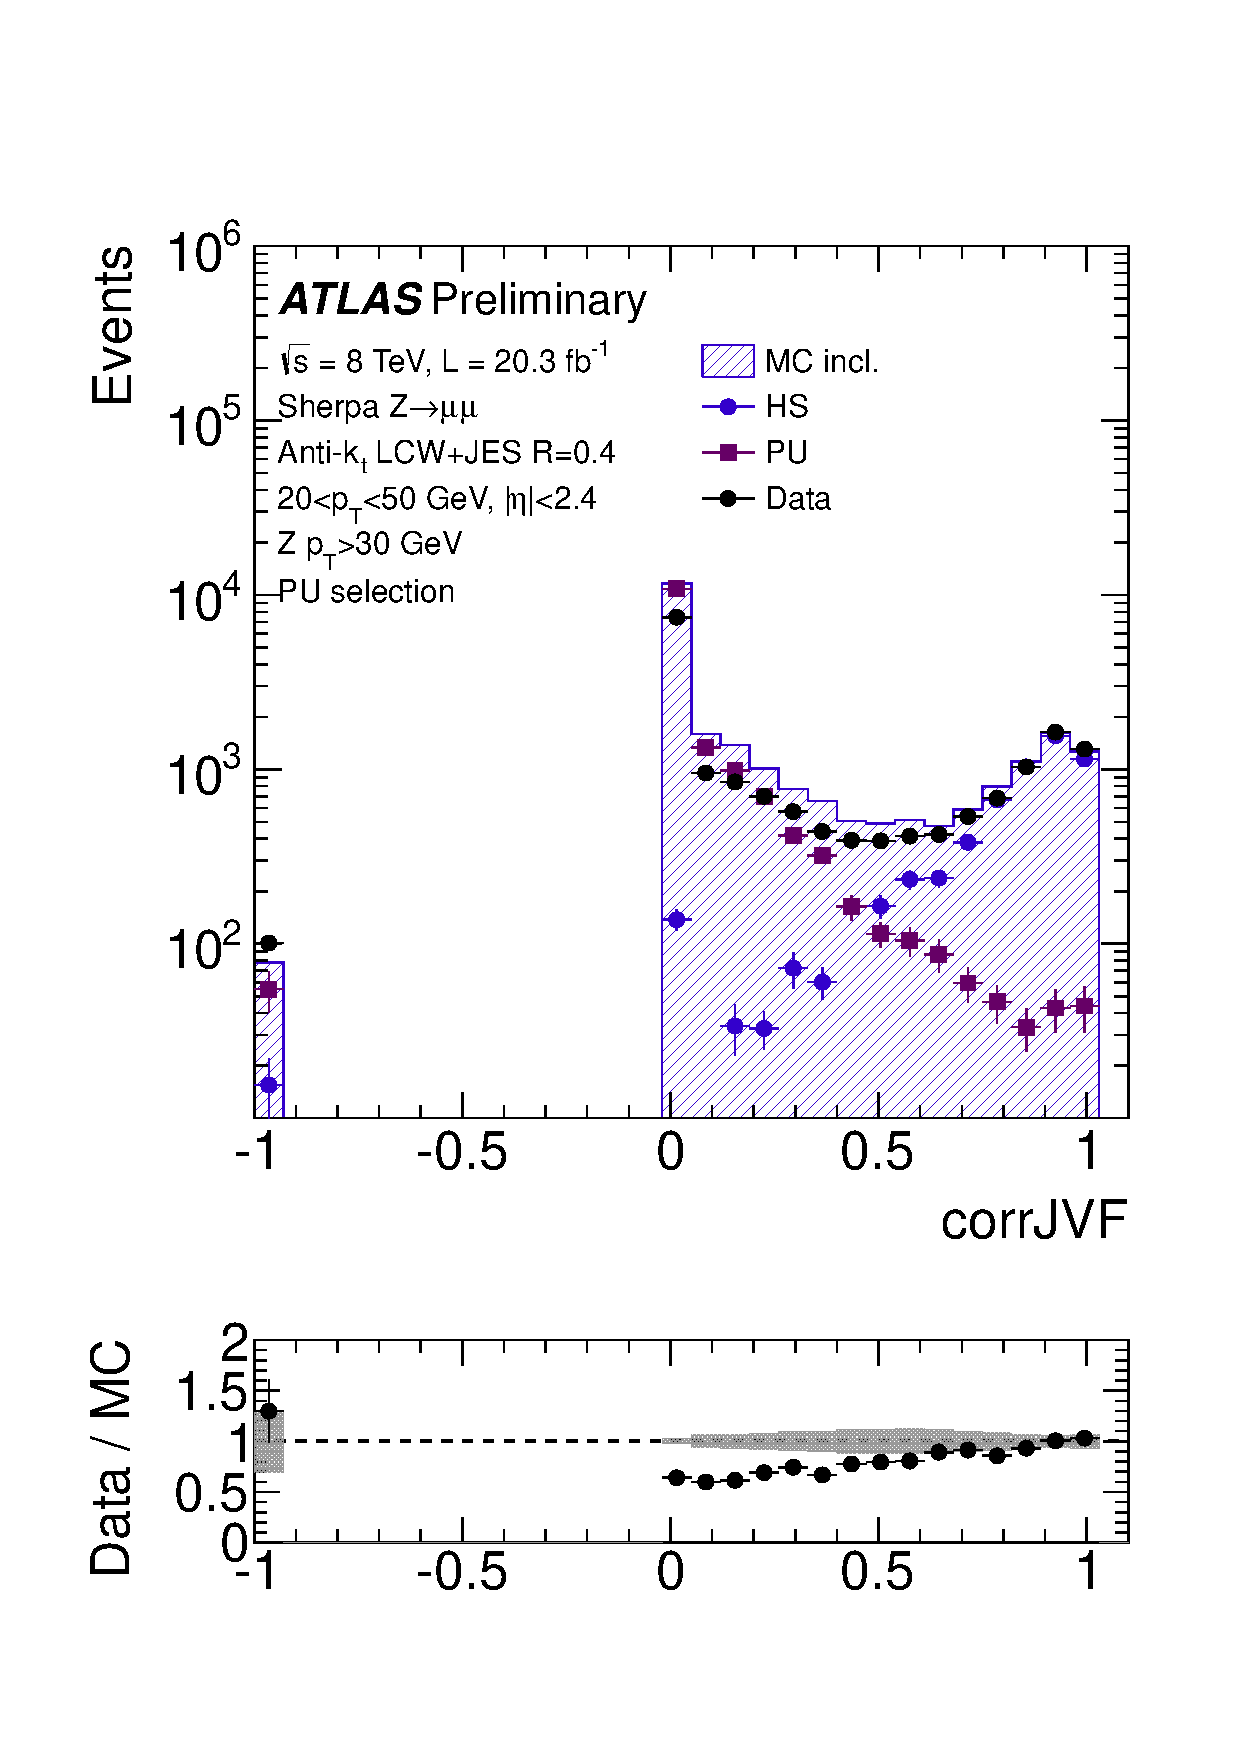
\includegraphics[width= 0.31\textwidth]{corrJVF_PUenriched_noFit}
    \label{fig:Zmumu_PUenriched_cJVF_nofit}
  }
  \subfigure[]{
      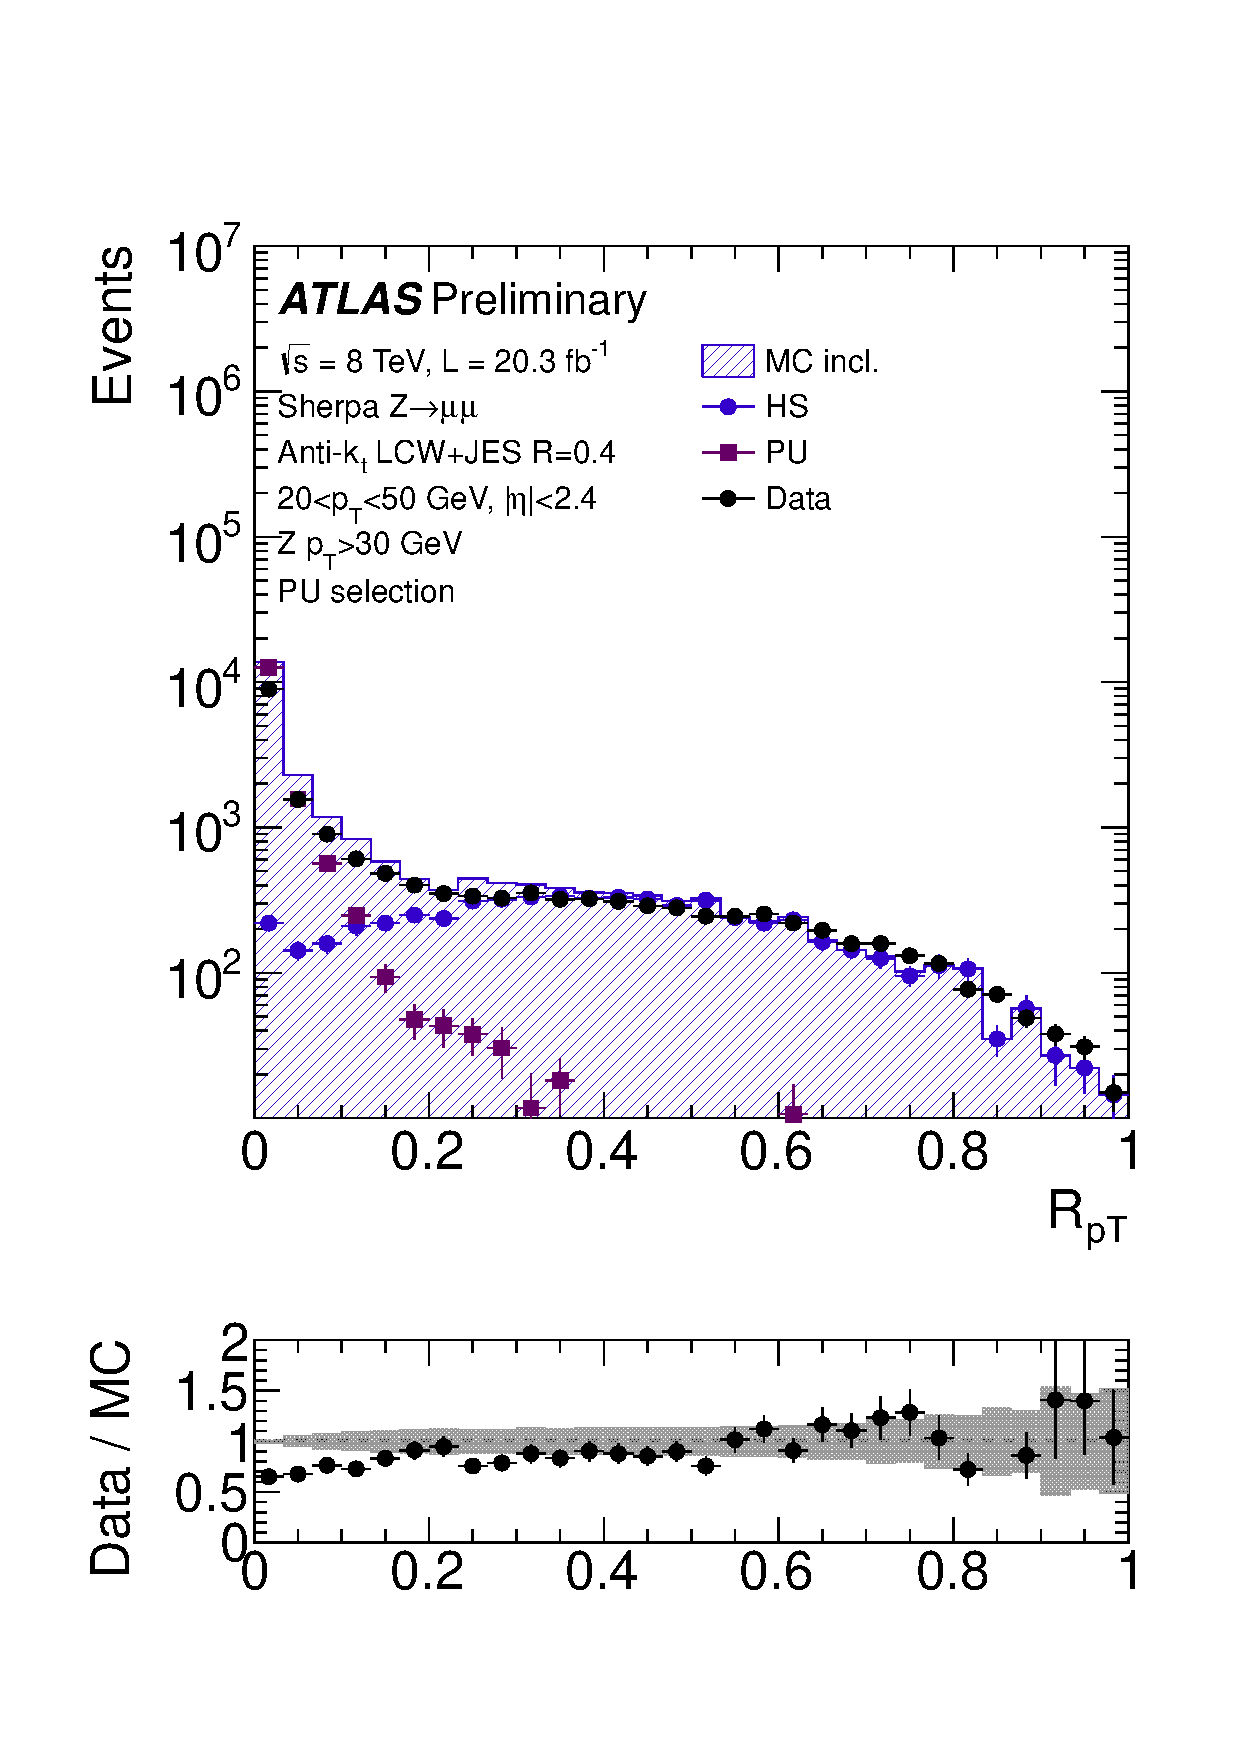
\includegraphics[width= 0.31\textwidth]{RpT_PUenriched_noFit}
    \label{fig:Zmumu_PUenriched_RpT_nofit}
  }
  \subfigure[]{
      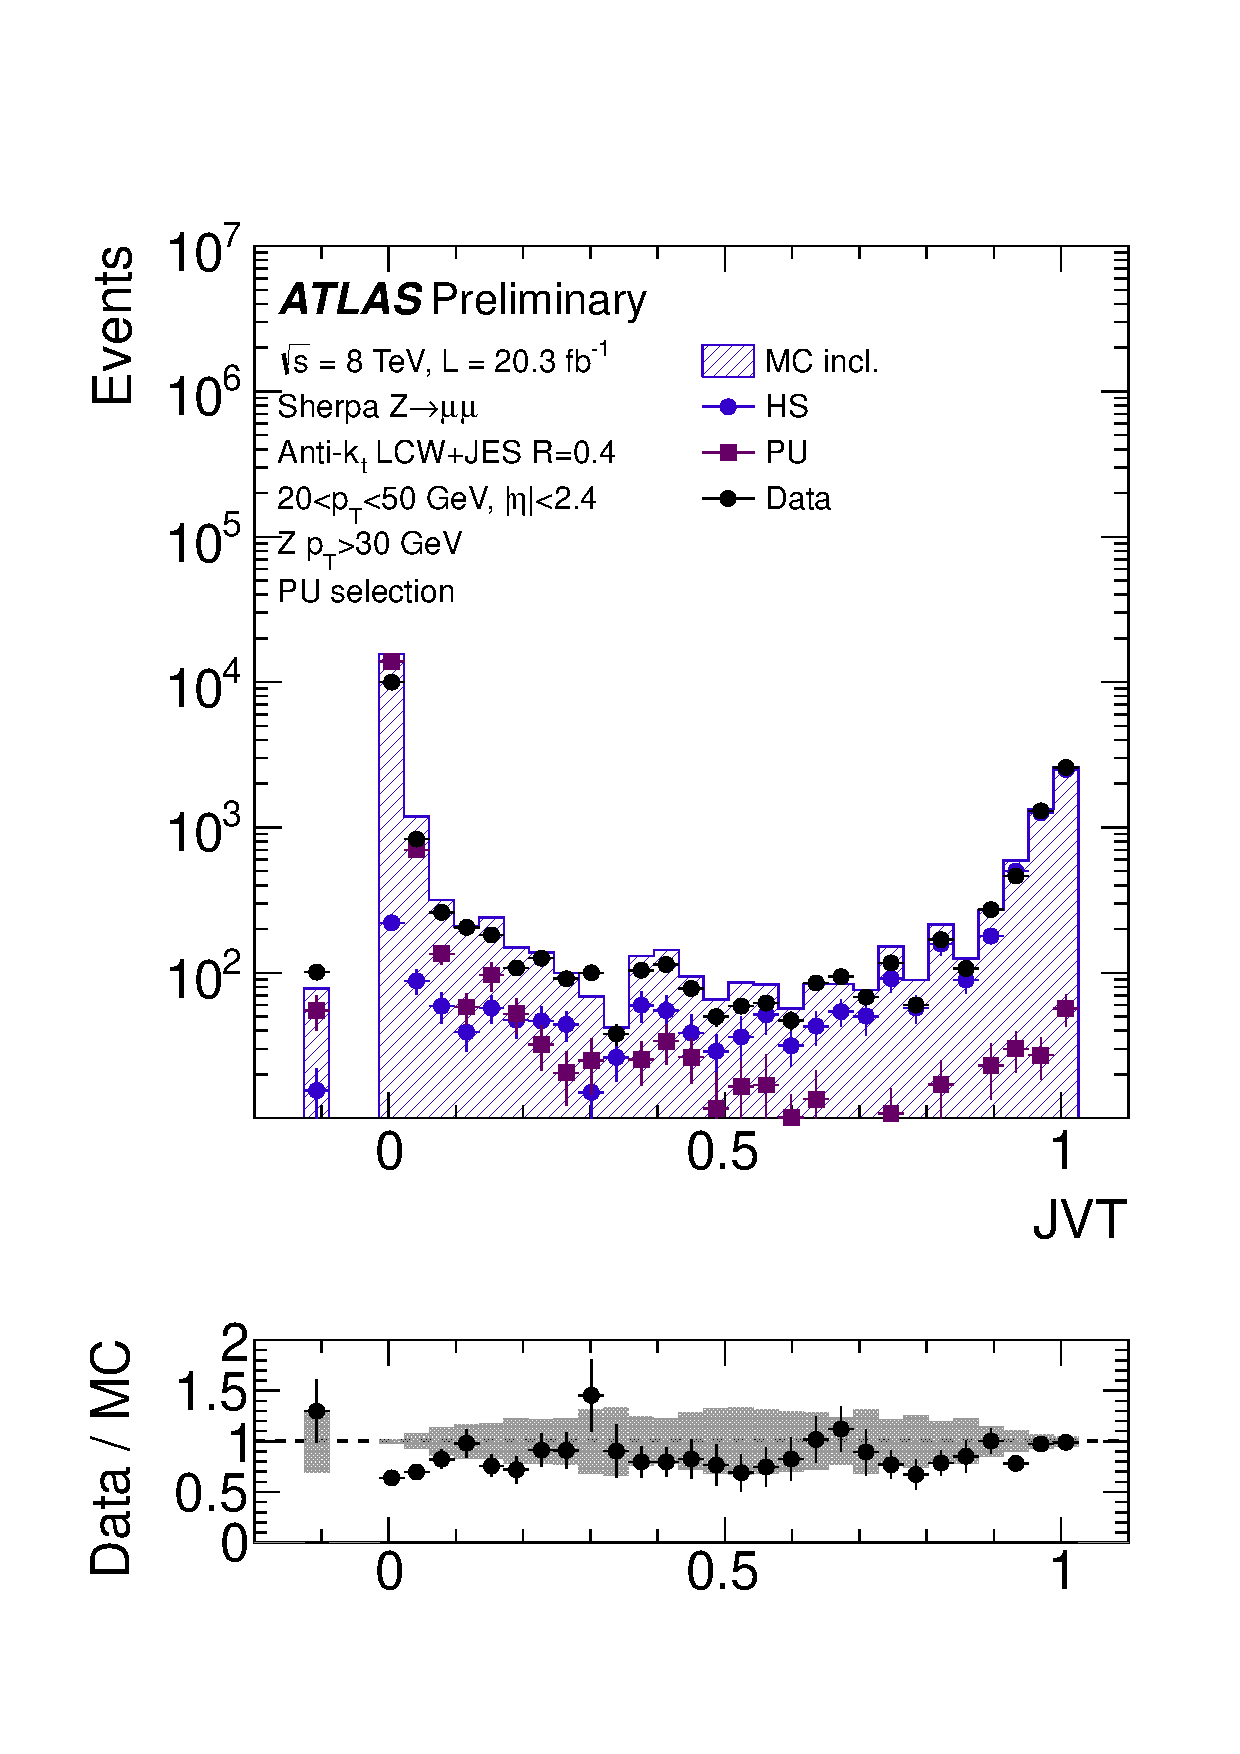
\includegraphics[width= 0.31\textwidth]{JVT_PUenriched_noFit}
    \label{fig:Zmumu_PUenriched_JVT_nofit}
  }
  \subfigure[]{
      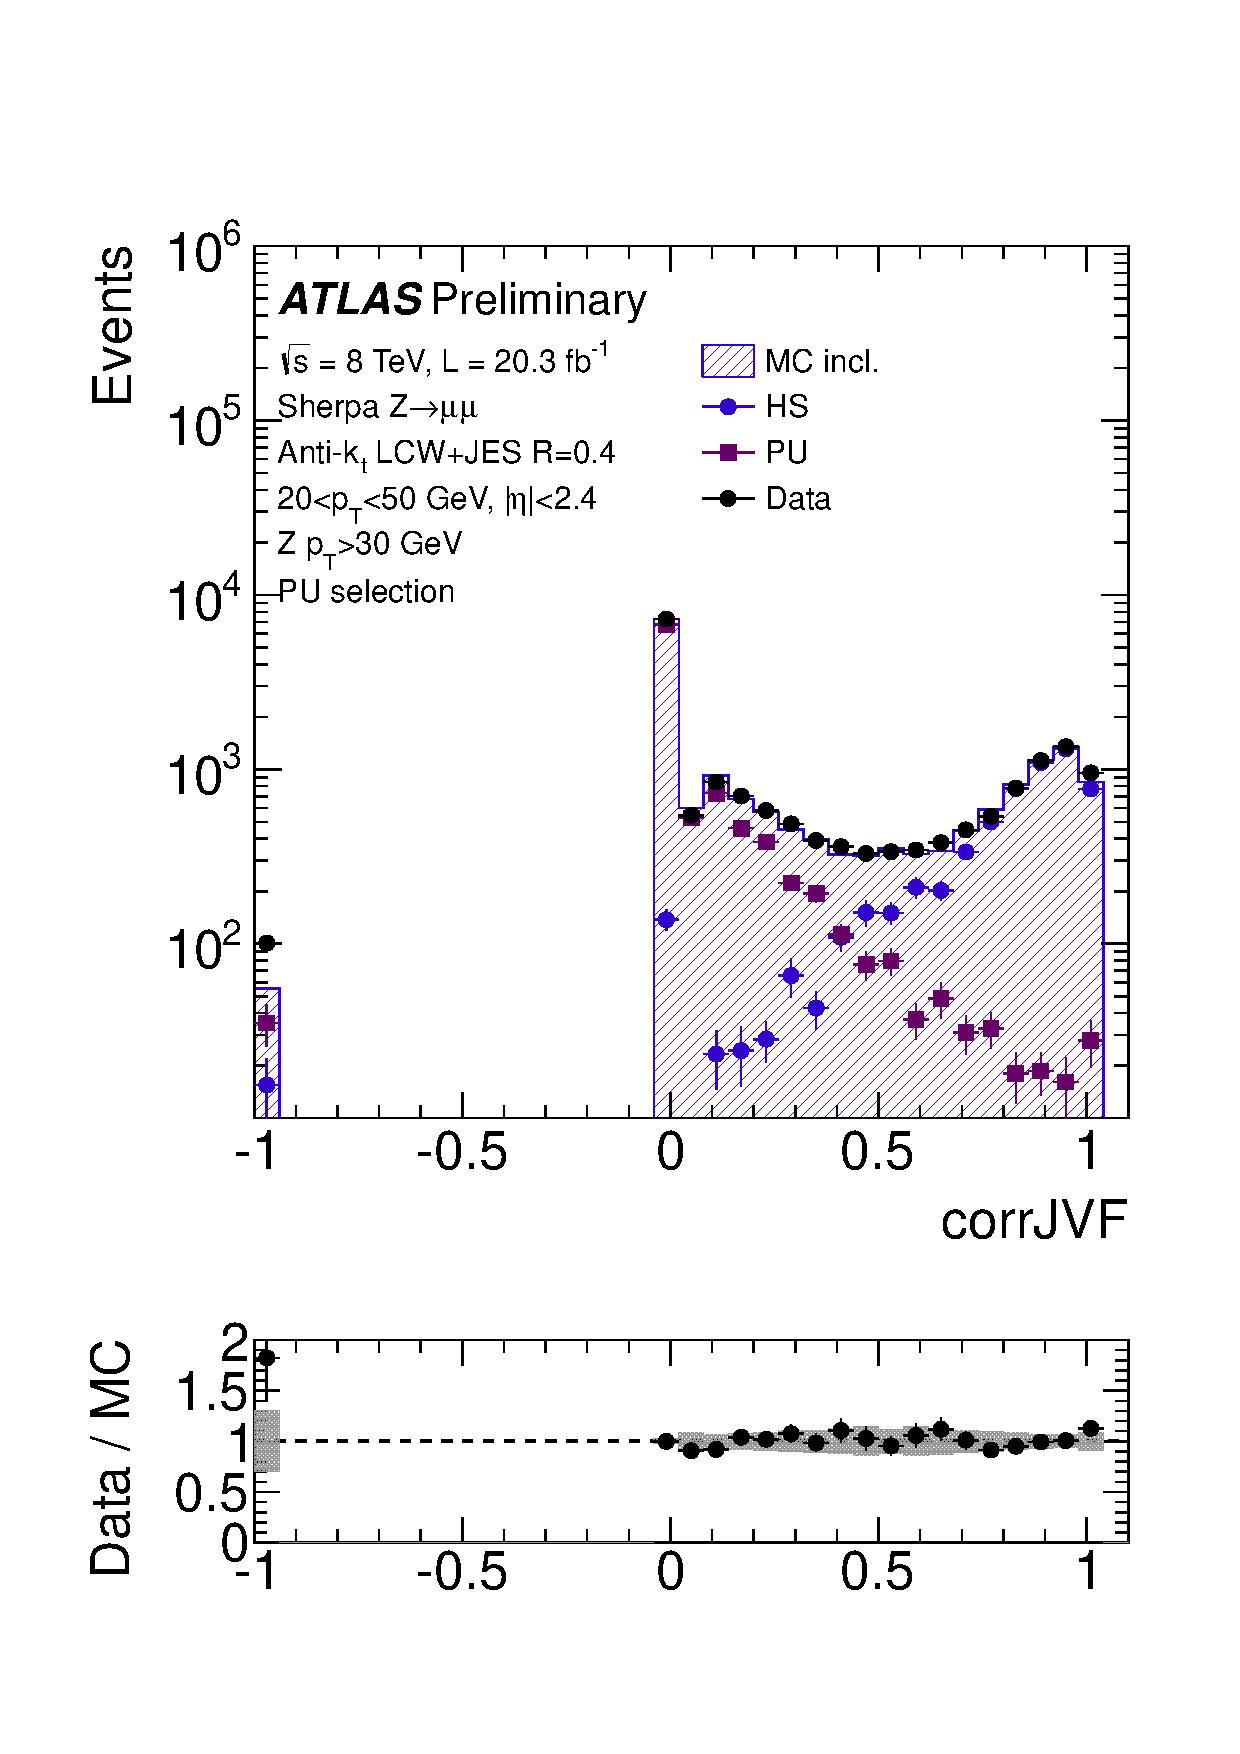
\includegraphics[width= 0.31\textwidth]{corrJVF_PUenriched}
    \label{fig:Zmumu_PUenriched_cJVF}
  }
  \subfigure[]{
      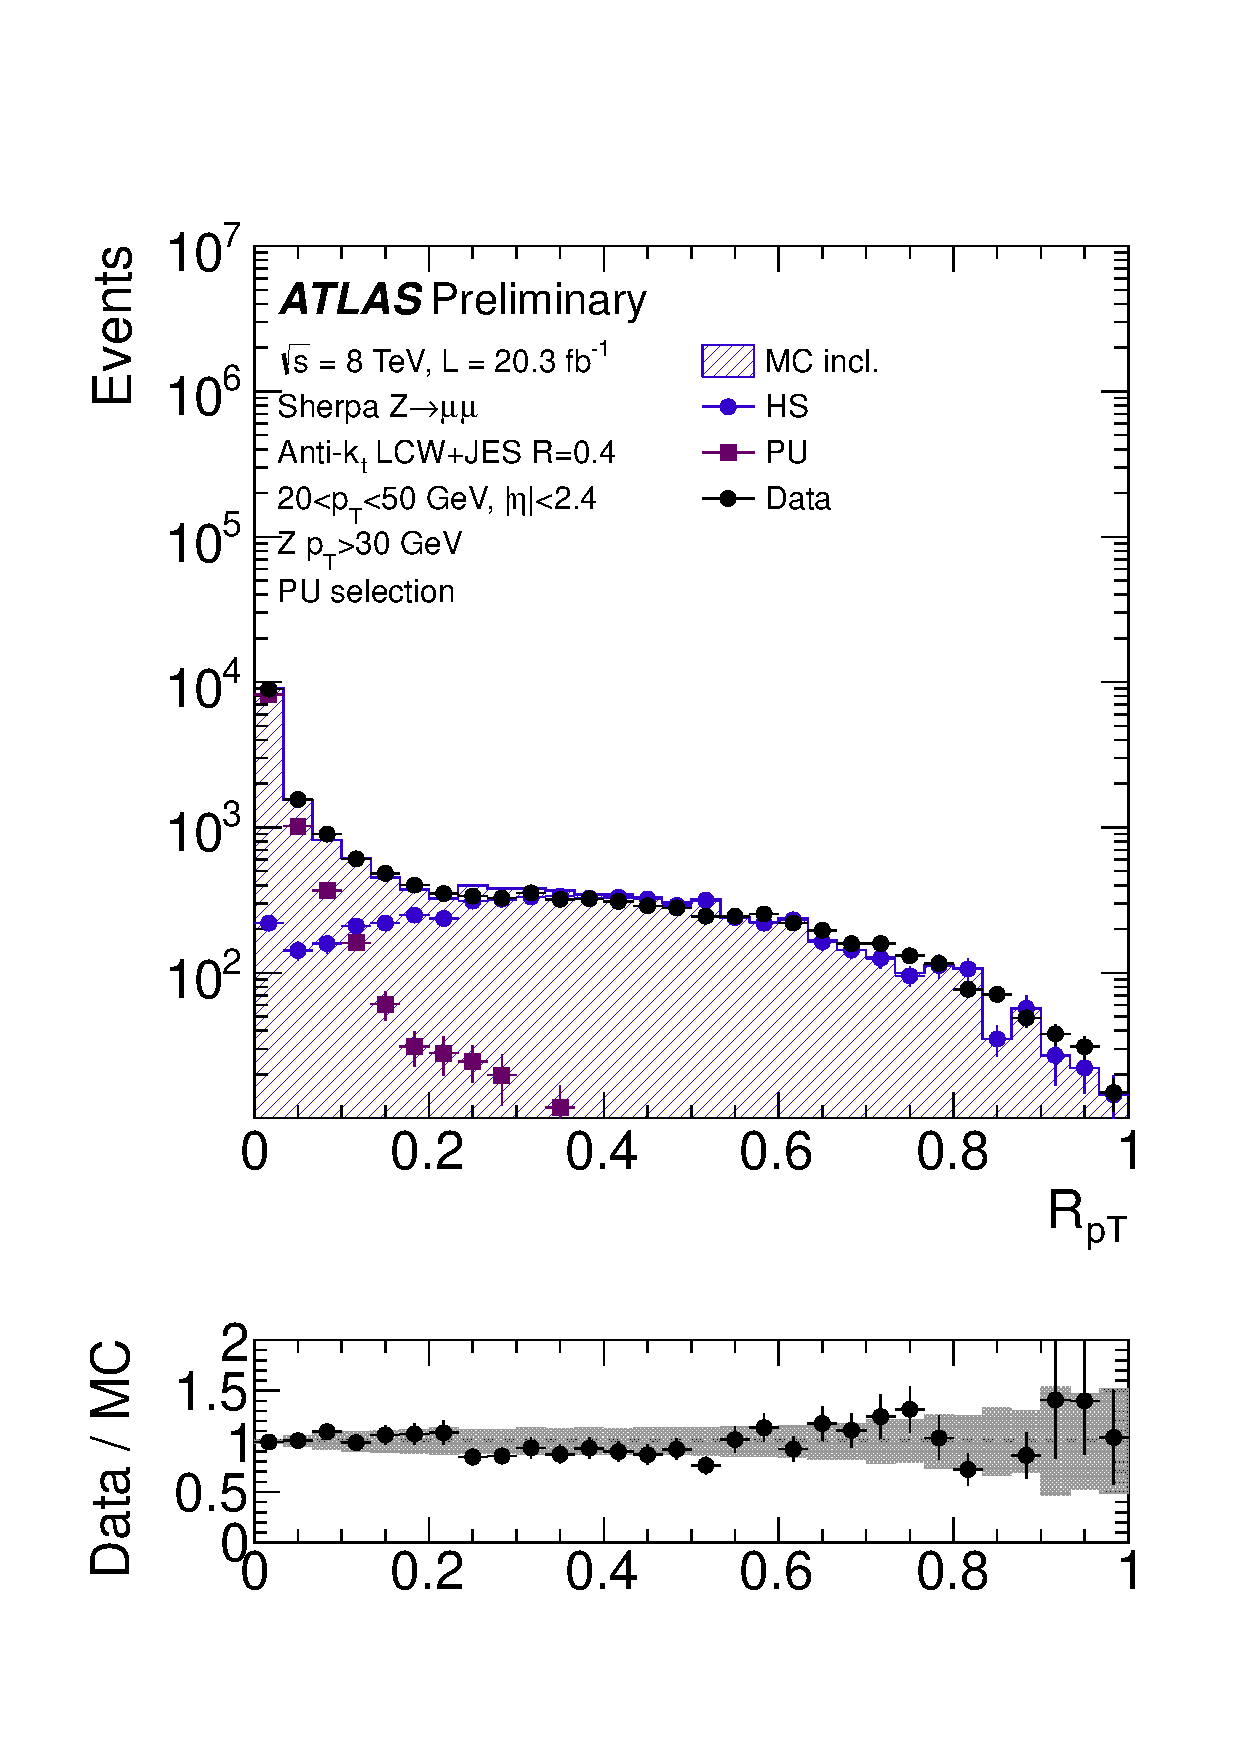
\includegraphics[width= 0.31\textwidth]{RpT_PUenriched}
    \label{fig:Zmumu_PUenriched_RpT}
  }
  \subfigure[]{
      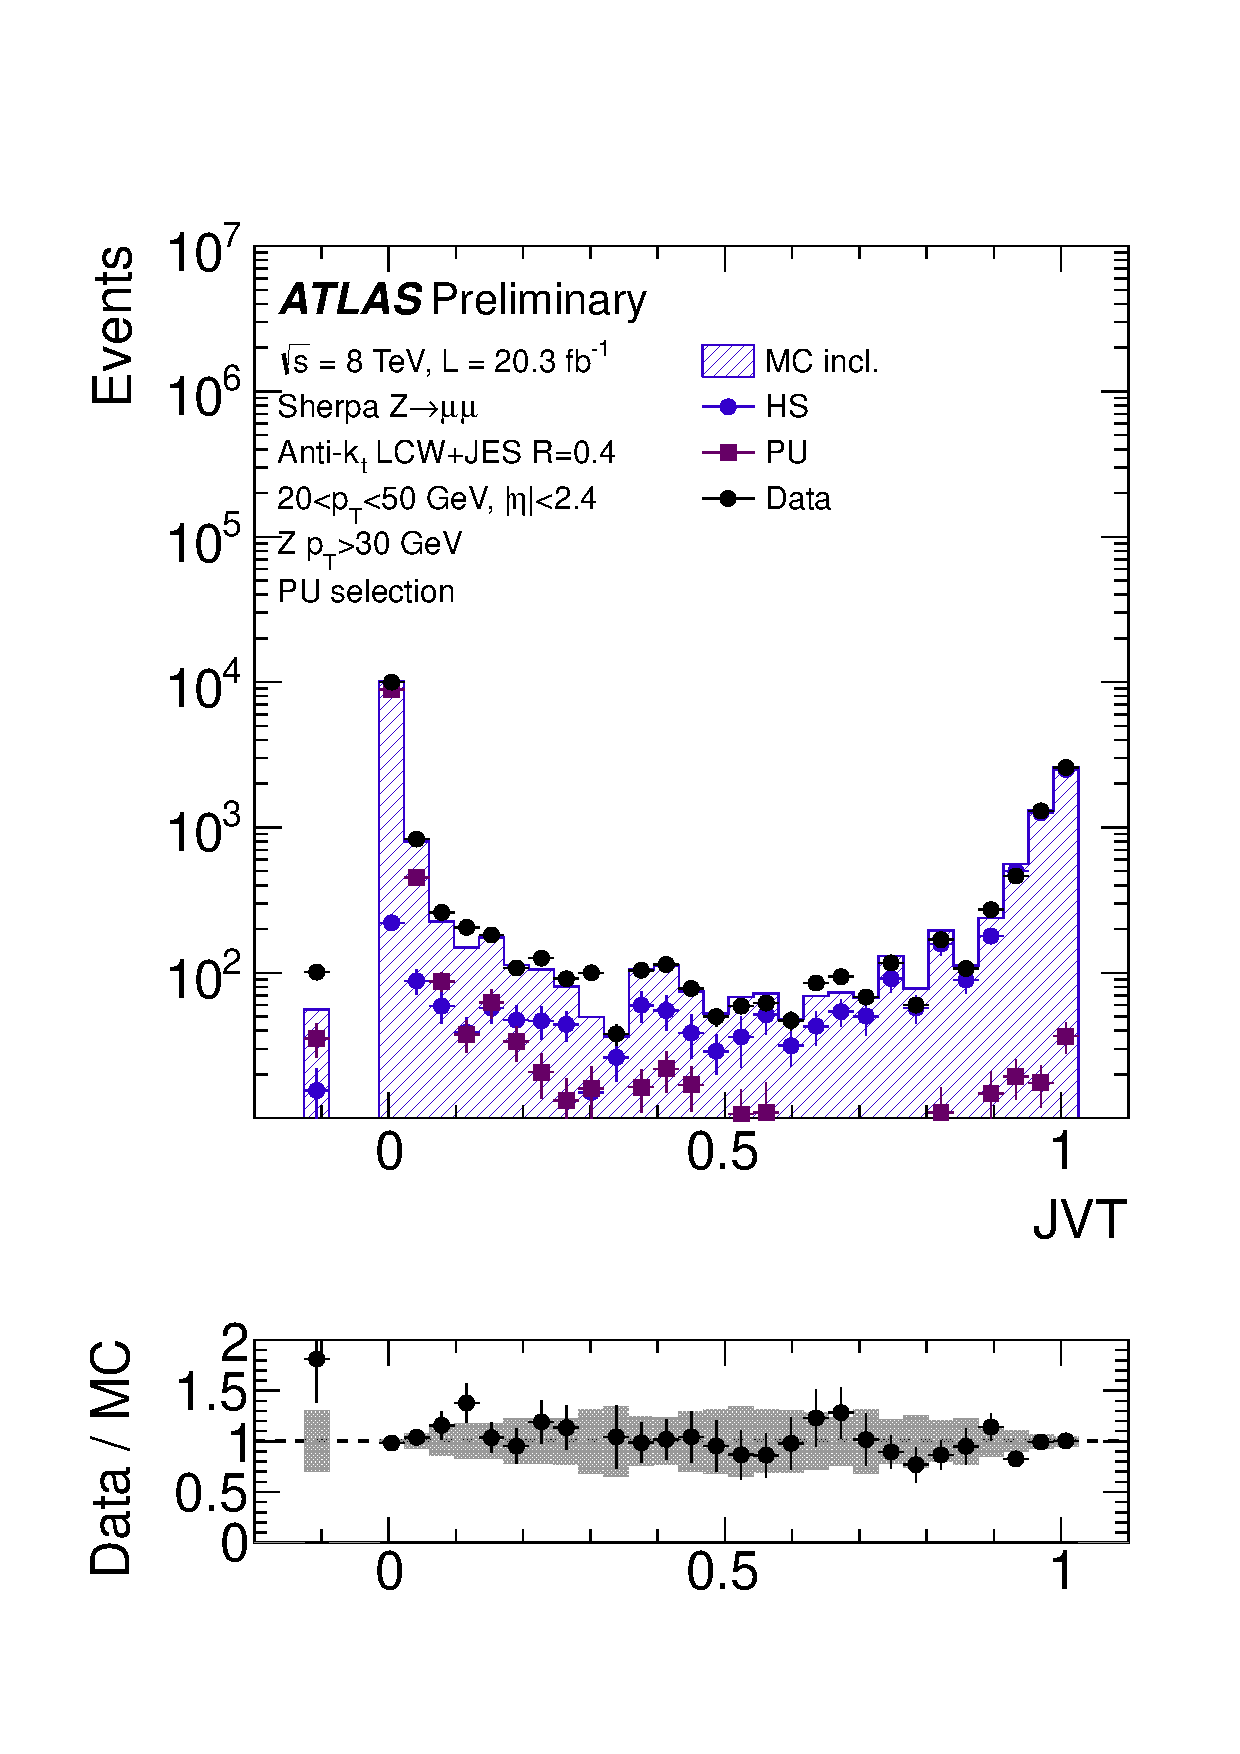
\includegraphics[width= 0.31\textwidth]{JVT_PUenriched}
    \label{fig:Zmumu_PUenriched_JVT}
  }
  \caption{Distributions of \cJVF (a), \RpT (b) and \JVT (c) using the event selection enhanced in pileup jets.  
%      While the
%      hard-scatter dominated tail are well described, an overestimate
%      of the pileup contribution in the simulation is observed. 
      In Figures (d), (e) and 
      (f) the pileup jet contribution in the simulation it fit to the data, while keeping the hard-scatter jets at their nominal
      normalization. 
  }
  \label{fig:Zmumu_PUenriched}
\end{figure}
%------------------------
Next, a sample further enriched in pileup jets 
is obtained by imposing the same selection criteria as in Figure~\ref{fig:Zmumu_HS} but replacing the back-to-back requirement with 
the criterion $|\Delta \phi(\Zboson,{\rm jet})|<1.2$. 
The data to simulation comparison for \cJVF, \RpT and \JVT for this selection of jets 
is shown in Figures~\ref{fig:Zmumu_PUenriched_cJVF_nofit},\ref{fig:Zmumu_PUenriched_RpT_nofit} and \ref{fig:Zmumu_PUenriched_JVT_nofit}.
While the pileup dominated regions in the three distributions are overestimated in simulation, 
the hard-scatter dominated tails of the distributions are reasonably well reproduced. 

As a cross-check, we use the simulated sample of jets passing this event selection to form a template of hard-scatter and another of pileup jets. 
We then perform a binned maximum likelihood fit to fit the pileup template to the data, while keeping the hard-scatter contribution at its
nominal value from Figures~\ref{fig:Zmumu_PUenriched_cJVF_nofit}, \ref{fig:Zmumu_PUenriched_RpT_nofit} and \ref{fig:Zmumu_PUenriched_JVT_nofit}. 
The post-fit distributions of \cJVF, \RpT and \JVT are shown in Figures~\ref{fig:Zmumu_PUenriched_cJVF},~\ref{fig:Zmumu_PUenriched_RpT} and \ref{fig:Zmumu_PUenriched_JVT}, 
respectively. With the rescaled pileup contribution, a good agreement between data and simulation is observed in the pileup and hard-scatter dominated 
regions as well as in the transition regions.  


In conclusion, the \cJVF, \RpT and \JVT distributions of hard-scatter jets are found to be well modeled using different event selections. 
The pileup jet rate, however, 
is found to be overestimated in simulation. 

\subsection{Validation for b-tagged jets using \ttbar events}
%-------------------------------------
\begin{figure}[!htbp]
  \centering
  \subfigure[]{
      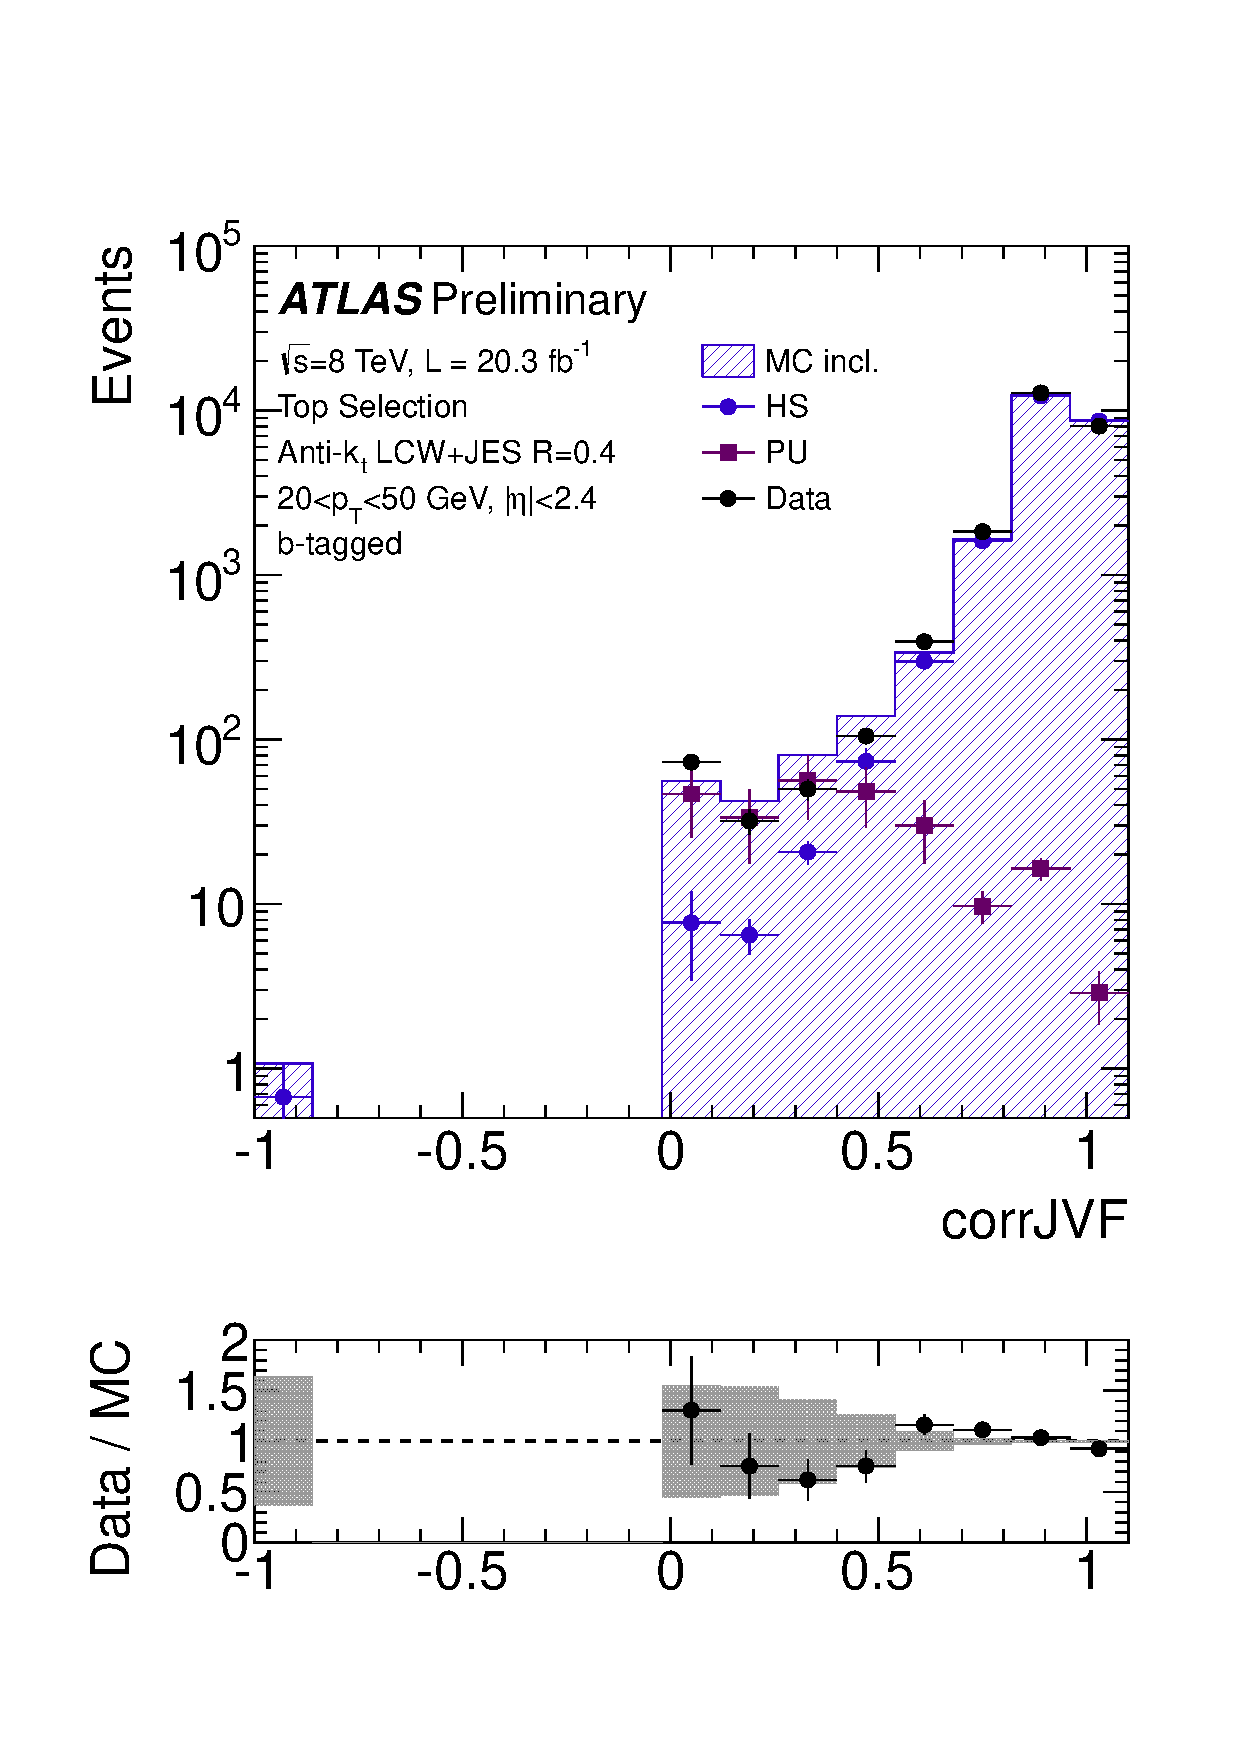
\includegraphics[width= 0.31\textwidth]{corrJVF_TopSel_btag_DataToMC}
      \label{fig:Top_btag_corrJVF}
  }
  \subfigure[]{
      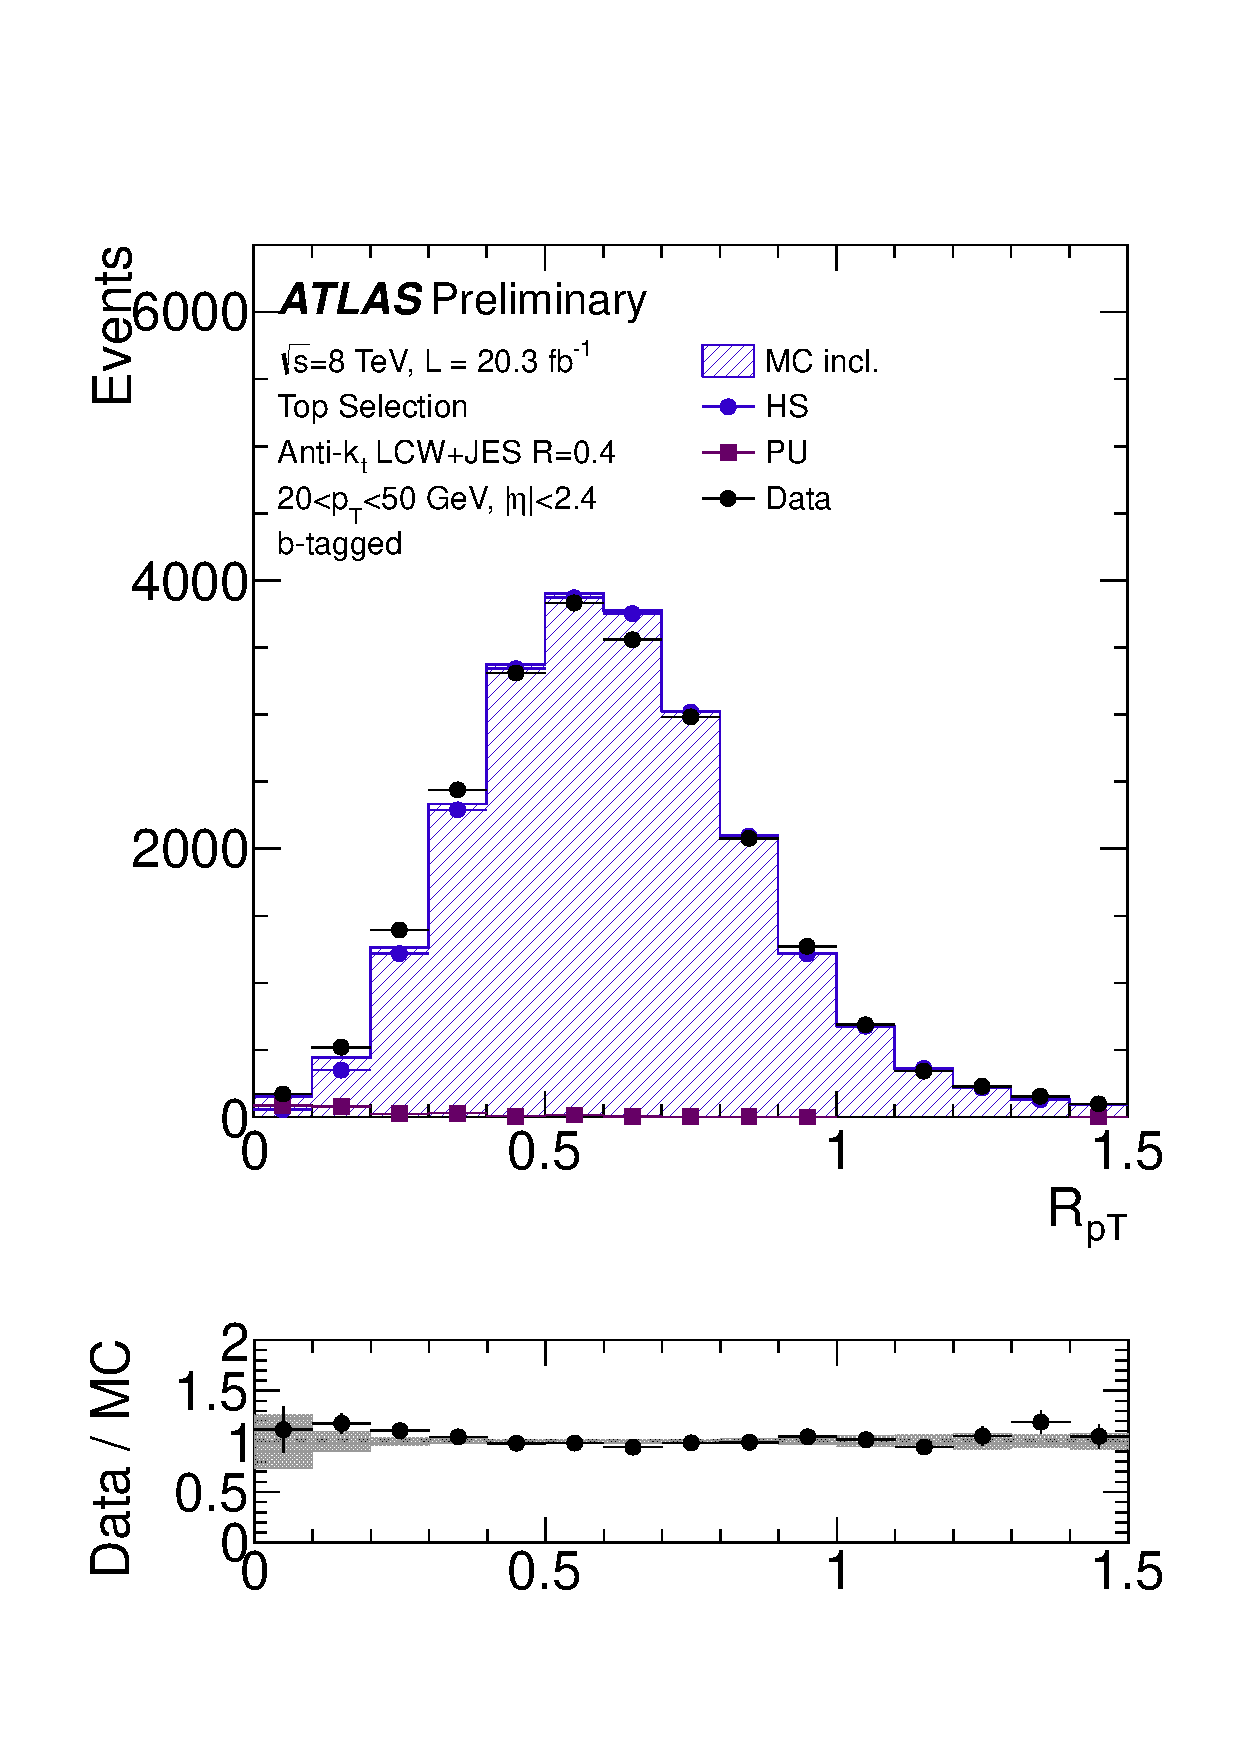
\includegraphics[width= 0.31\textwidth]{RpT_TopSel_btag_DataToMC}
  \label{fig:Top_btag_RpT}
  }
  \subfigure[]{
      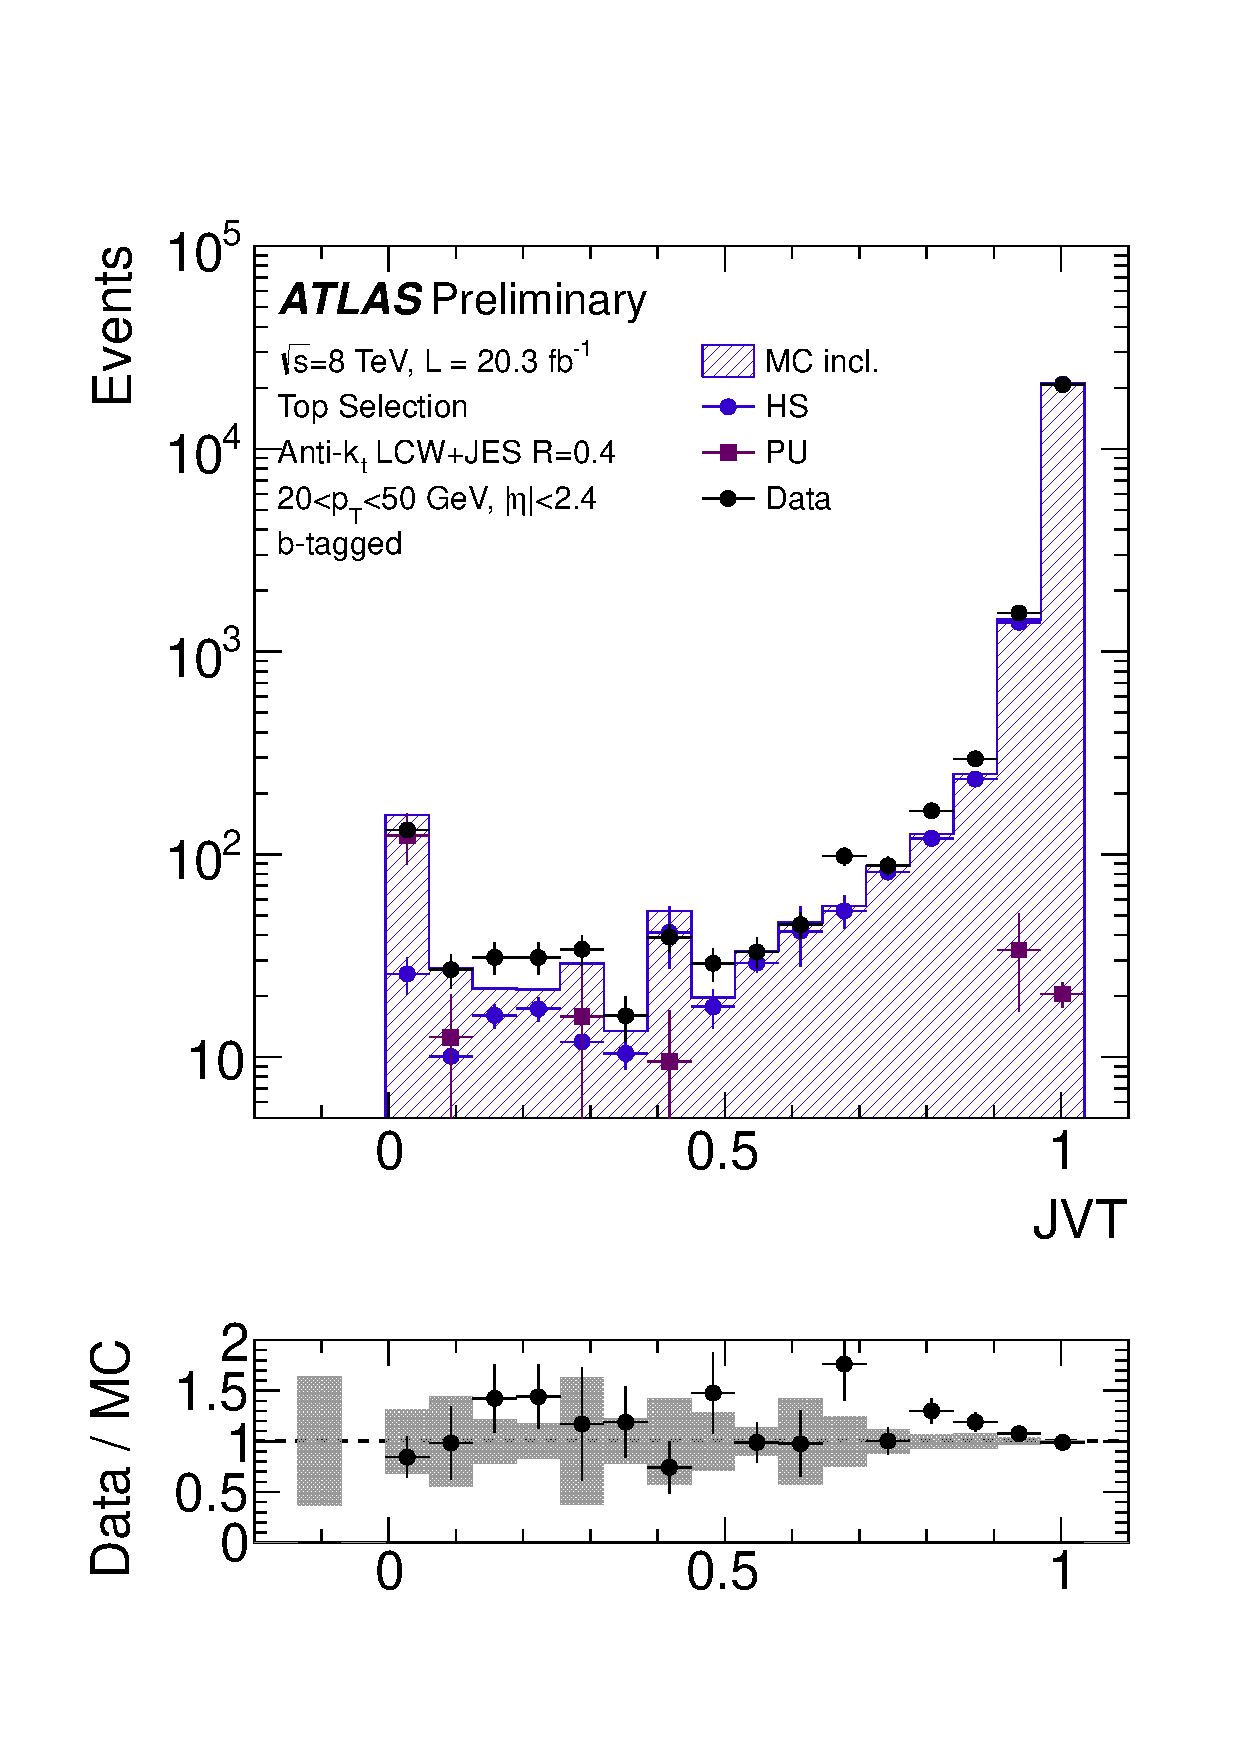
\includegraphics[width= 0.31\textwidth]{JVT_TopSel_btag_DataToMC}
  \label{fig:Top_btag_JVT}
  }
  \caption{The distributions of \cJVF, \RpT and \JVT for the two b-tagged jets with $20<\pT<50\GeV$ and $|\eta|<2.4$ in  \ttbar dominated events. 
  The blue shaded histograms representing the inclusive simulation are subdivided in its hard-scatter jet and pileup jet contributions
  using blue and magenta markers respectively. The gray band in the ratio plot represents the statistical uncertainty in the simulation. 
  The simulation is normalized to the area of the data.}
  \label{fig:Top_btag}
\end{figure}
%------------------------

Figure~\ref{fig:Top_btag} shows a comparison of the data and the simulation for the two b-tagged jets with $20<\pT<50\GeV$ and $|\eta|<2.4$ in \ttbar enriched events, 
using the selection described 
in Section~\ref{sec:eventSel}.
In simulation this event selection is $92\%$ pure in \ttbar events. A reasonable agreement is observed for the distributions of \cJVF, \RpT and
\JVT. 

%--------------------------------------------------------
\subsection{\JVT calibration}
%--------------------------------------------------------
\label{subsec:calibration}
We use jets in $\Zboson(\to\mu\mu)$+jets events to measure the hard-scatter jet efficiency for \JVT in data, exploiting a tag-and-probe procedure 
similar to that described in 
Ref.~\cite{CMS-PAS-JME-13-005}. Using the leading jet recoiling against the 
\Zboson boson as a probe, a signal region of hard-scatter jets is defined as the back-to-back region specified as $|\Delta \phi (\Zboson, {\rm jet})| > 2.8$. 
The pileup contamination in the signal region is estimated from a pileup control region, 
based on the assumption that the $|\Delta \phi (\Zboson, {\rm jet})|$ distribution is
flat for pileup jets. It is observed in simulation that this assumption is not well justified for the pileup jet definition given in Section~\ref{sec:jets}. Instead, the 
strict requirement for pileup jets to be isolated within $\Delta R>0.6$ from any truth jet biases the $|\Delta \phi (\Zboson, {\rm jet})|$ distribution in the back-to-back region. 
To avoid this problem, the isolation requirement 
for pileup jets is loosened to $\Delta R>0.4$ (for which an unbiased $|\Delta \phi (\Zboson, {\rm jet})|$ distribution is found in simulation) 
for this efficiency measurement. The pileup control region is defined as $|\Delta \phi (\Zboson, {\rm jet})|<1.2$ (as in Figure~\ref{fig:Zmumu_PUenriched}), from which the pileup contamination 
in the signal region $N_{\rm PU}^{\rm signal}$ is estimated as 
\begin{eqnarray}
    {N_{{\rm PU}}^{\rm signal}(|\Delta \phi|>2.8) = [N_{\rm j}^{\rm control}(|\Delta \phi|<1.2) - N_{\rm HS}(|\Delta \phi|<1.2)] \cdot (\pi - 2.8)/1.2},
\end{eqnarray}
where $N_{\rm j}^{\rm control}(|\Delta \phi|<1.2)$ is the number of jets in the control region in the data. In simulation, the control region is about $70\%$ pure in pileup jets, so that 
a remaining hard-scatter jet contamination $N_{\rm{HS}}(|\Delta \phi|<1.2)$ needs to be subtracted from the data using simulation. 

The efficiency of a minimal \JVT requirement is then measured in bins of $\pT^{\rm ref} = \pT(\Zboson)$ as
\begin{eqnarray}
    \varepsilon = \frac{N_{\rm j}^{\rm pass} - N_{\rm PU}^{\rm pass}}{N_{\rm j}^{\rm signal} - N_{{\rm PU}}^{\rm signal}} 
                  \approx 
                  \frac{N_{\rm j}^{\rm pass}}{N_{\rm j}^{\rm signal} - N_{{\rm PU}}^{\rm signal}},
\end{eqnarray}
where $N_{\rm j}^{\rm signal}$ and $N_{\rm j}^{\rm pass}$ denote respectively the number of jets in the signal region and the number of events in the signal region passing the minimal
\JVT requirement. Using simulation, the contamination of pileup jets in the signal region passing the \JVT cut $N_{\rm PU}^{\rm pass}$ is estimated to account for
to less than $0.3\%$ of $N_{\rm j}^{\rm pass}$ for the \JVT cut values considered and is thus ignored. 

%----------------------
\begin{figure}[!htbp]
  \centering
  \subfigure[]{
      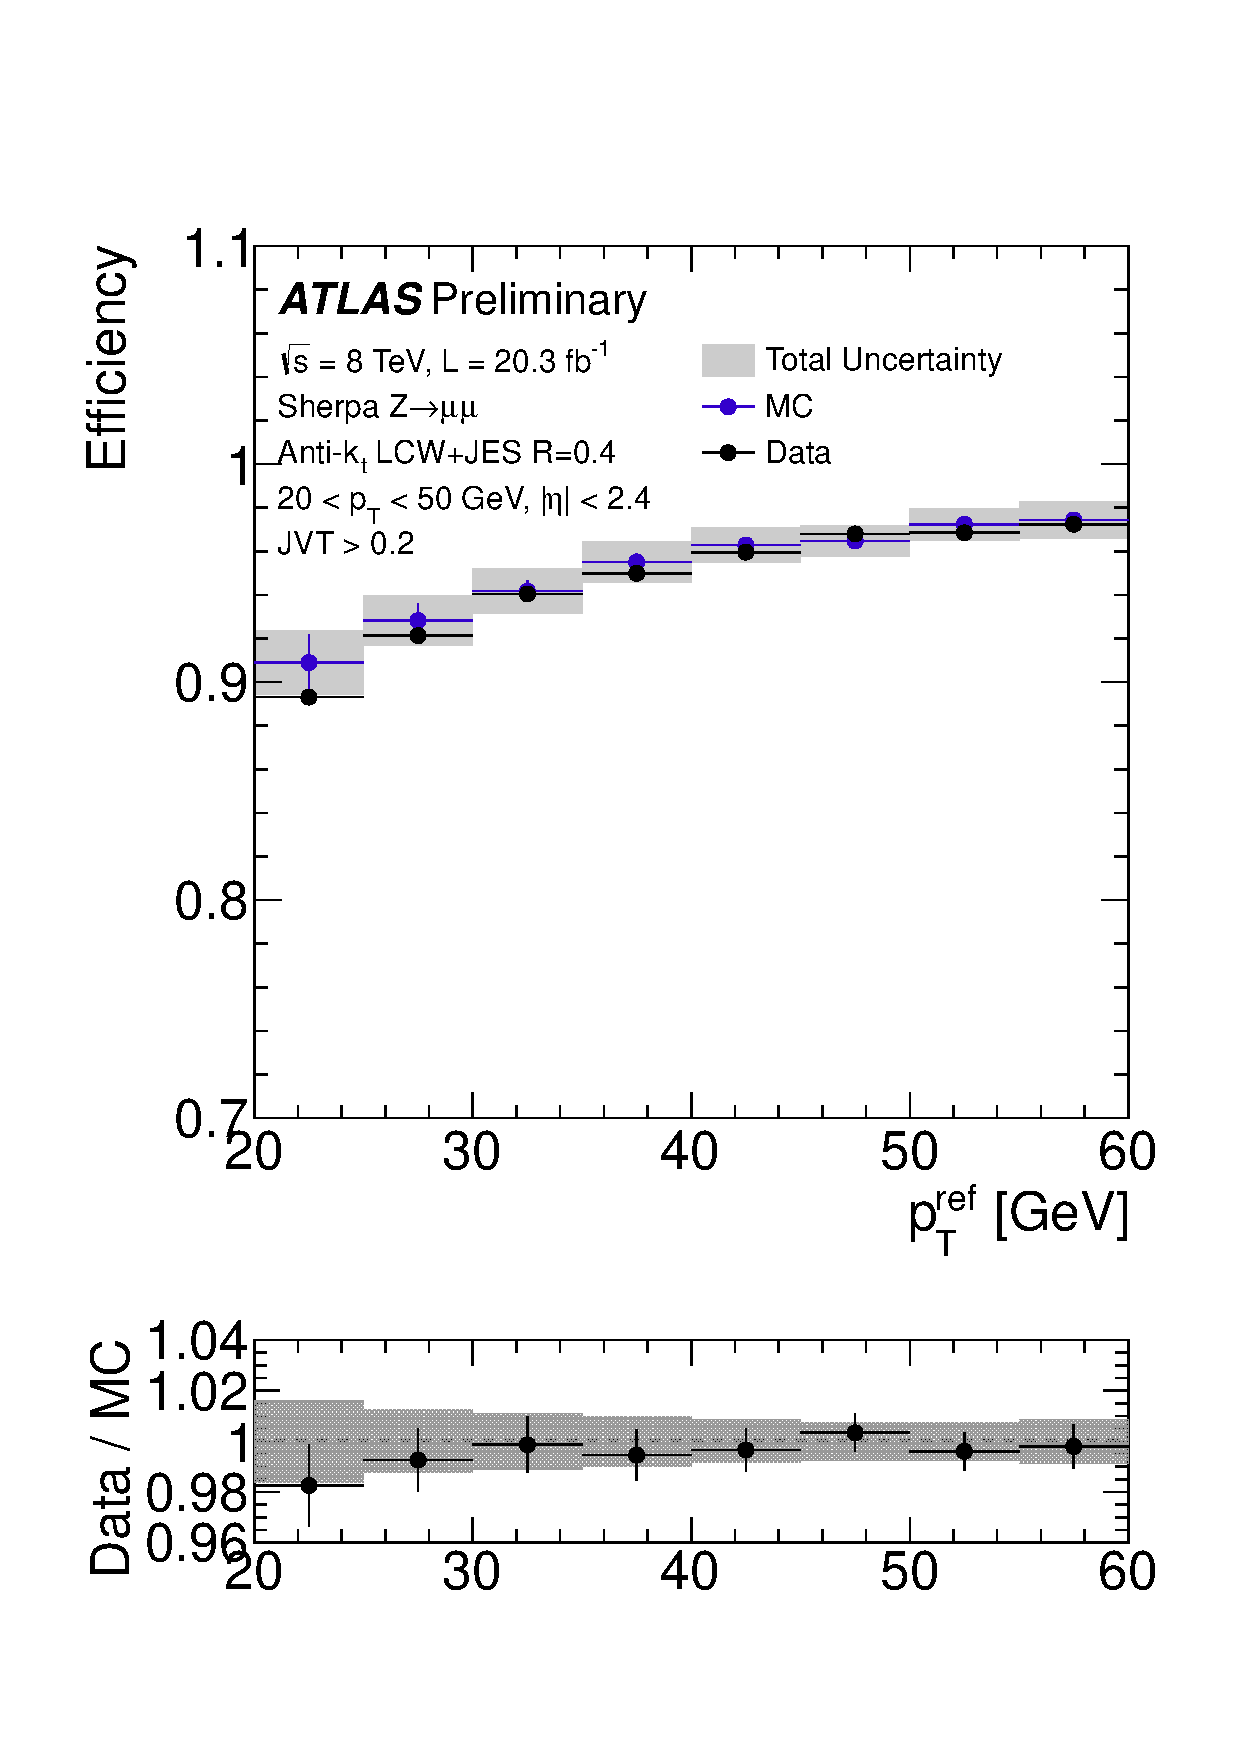
\includegraphics[width= 0.31\textwidth]{JVTCalibration_pTref_JVTgt0p2_ratio}
      \label{fig:JVTCal_0p2}
  }
  \subfigure[]{
      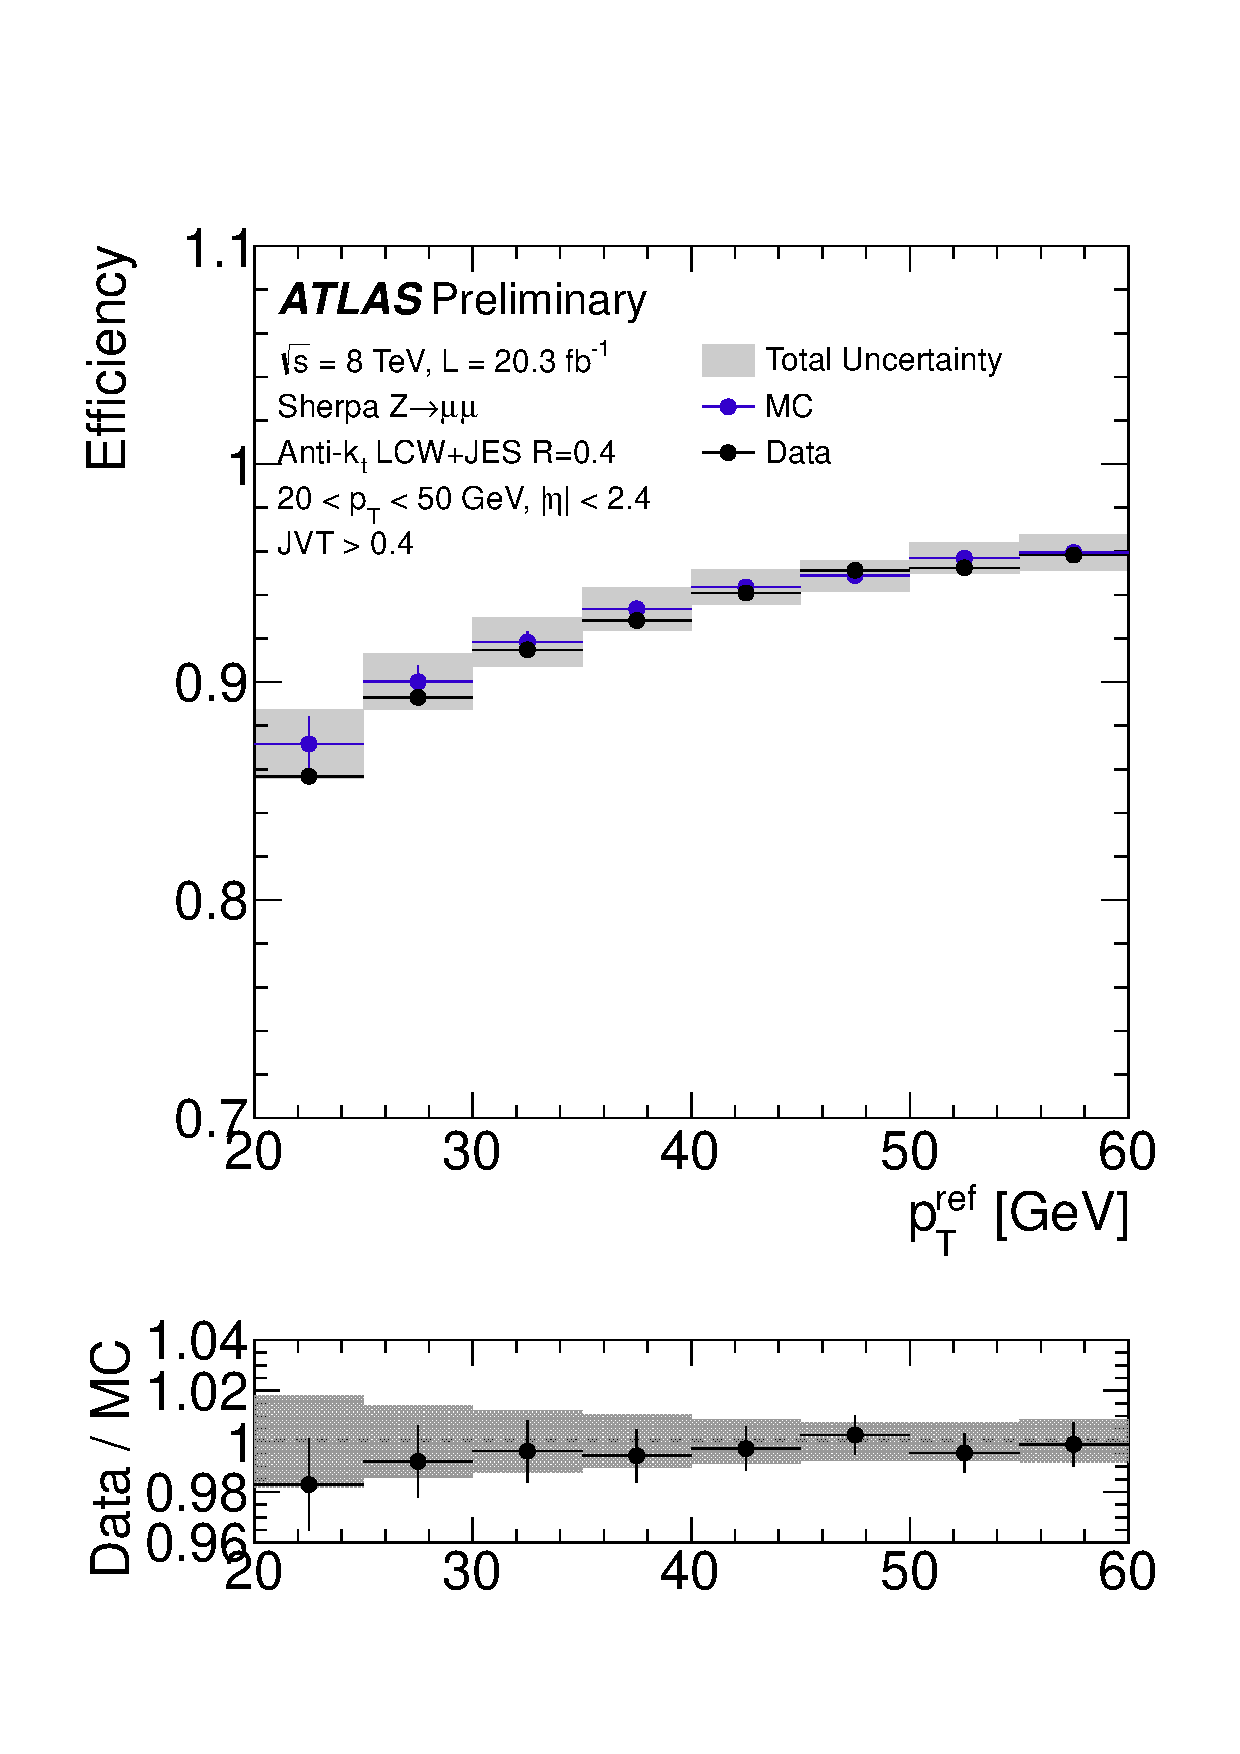
\includegraphics[width= 0.31\textwidth]{JVTCalibration_pTref_JVTgt0p4_ratio}
      \label{fig:JVTCal_0p4}
  }
  \subfigure[]{
      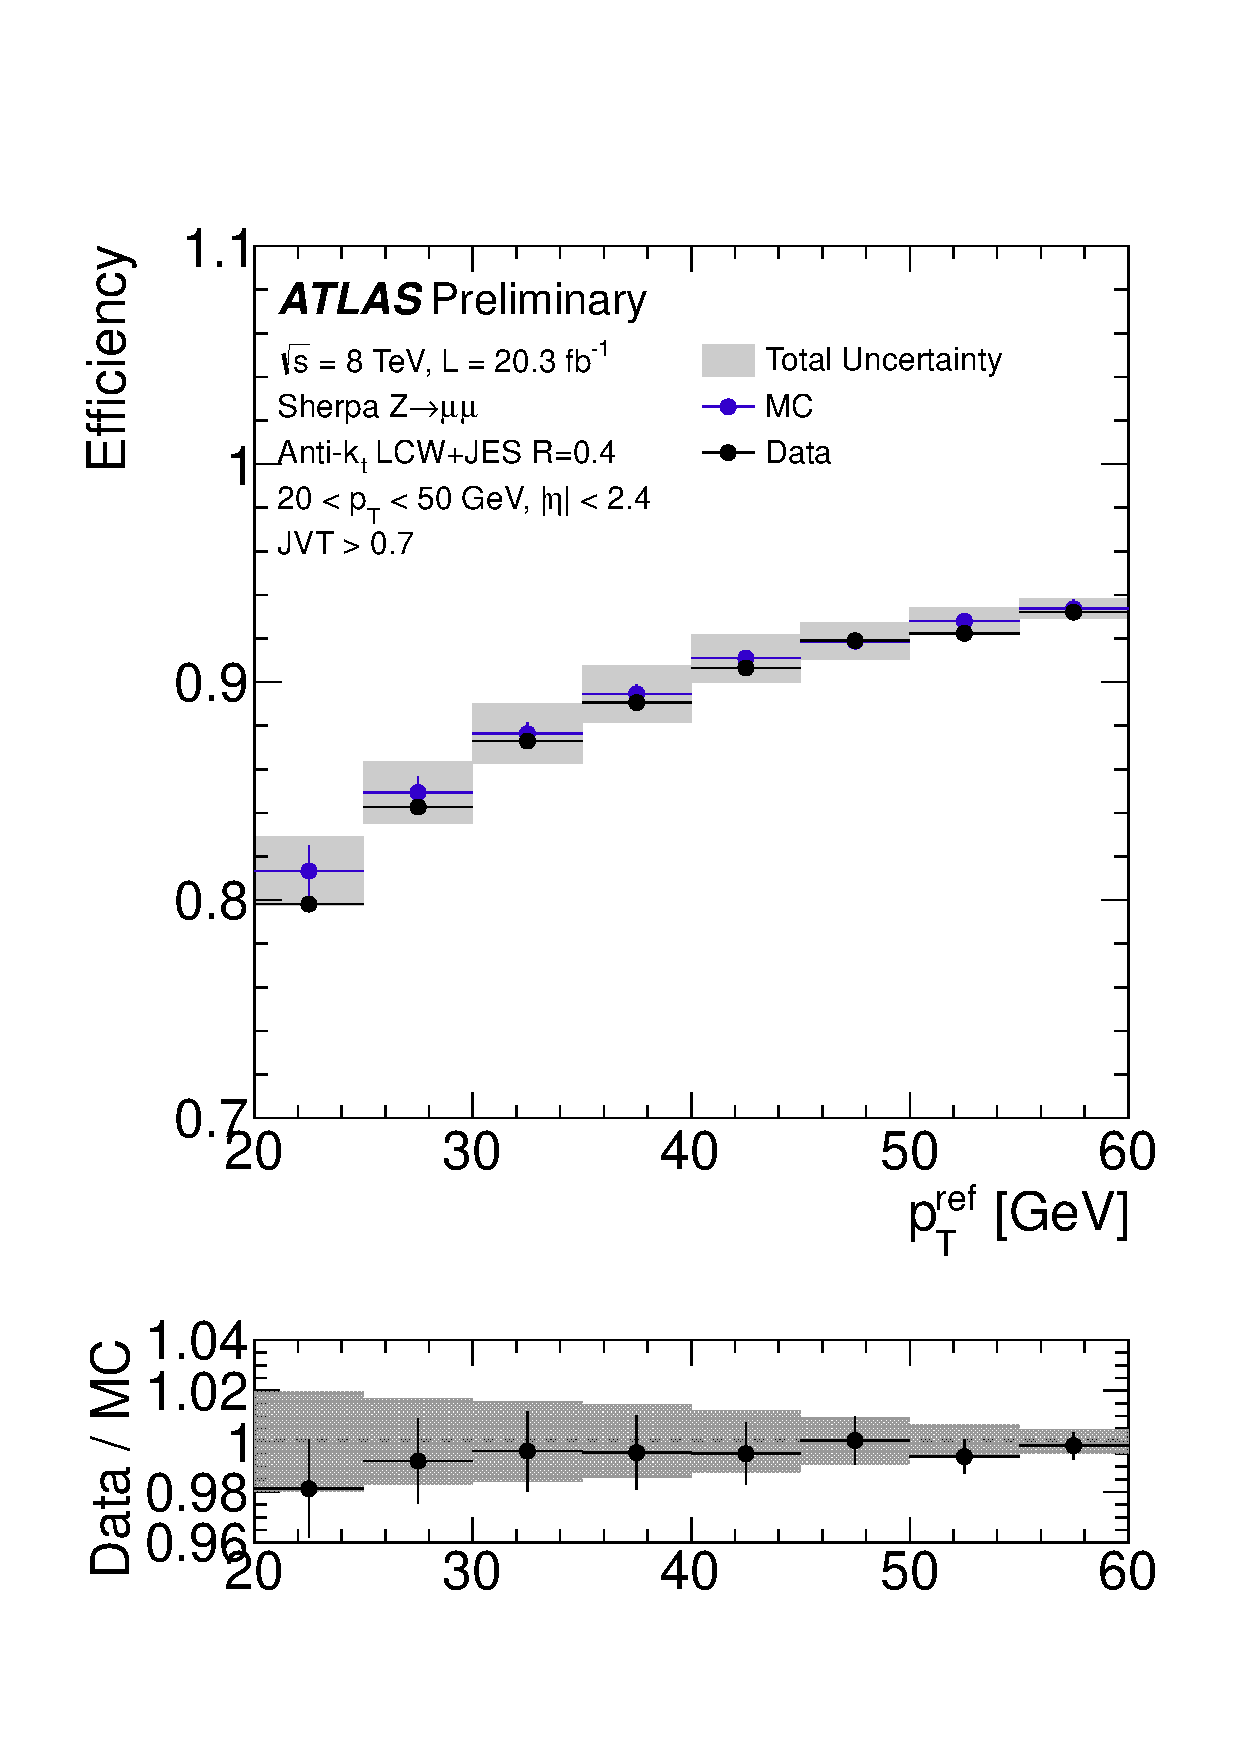
\includegraphics[width= 0.31\textwidth]{JVTCalibration_pTref_JVTgt0p7_ratio}
  \label{fig:JVTCal_0p7}
  }
  \caption{Efficiency of a $\JVT>0.2$ (a), $\JVT>0.4$ (b) and $\JVT>0.7$ (c) requirement as a function of $\pT^{\rm ref}$ in data and simulation.}
  \label{fig:JVTCalibration}
\end{figure}
%------------------------
Figures~\ref{fig:JVTCal_0p2}, \ref{fig:JVTCal_0p4} and~\ref{fig:JVTCal_0p7} show the jet efficiencies for  minimal \JVT requirements of 0.2, 0.4 and 0.7 respectively. 
Agreement is observed between data and simulation.
The simulation-to-data scale factors are consistent with unity within the uncertainties. 
The grey band reflects the total uncertainty on the efficiency in simulation, adding the statistical and the systematic uncertainties in quadrature. The systematic
uncertainty is comprised of the following components:
\begin{itemize}
    \item   Based on a data to MC comparison of the $|\Delta \phi (\Zboson, {\rm jet})|$ distribution for jets passing a minimal \JVT criterion, 
        we assign a conservative  30\% systematic uncertainty on $N_{\rm{HS}}(|\Delta \phi|<1.2)$ to account for a potential mis-modeling of the 
            the $\Delta \phi(\Zboson, {\rm jet})$ shape for hard-scatter jets.
        \item   A non-negligible difference in hard-scatter efficiency for fixed \JVT cuts is observed between the \Sherpa and the \Powheg $\Zboson(\to\mu\mu)$+jets MC samples, 
        attributed to the different fragmentation models used in \Sherpa and \PYTHIAeight. This difference, which is illustrated in Figure~\ref{fig:JVTeff_Syst},
            is taken as a systematic uncertainty.
\end{itemize}
%----------------------------
\begin{figure}[!htbp]
  \centering
  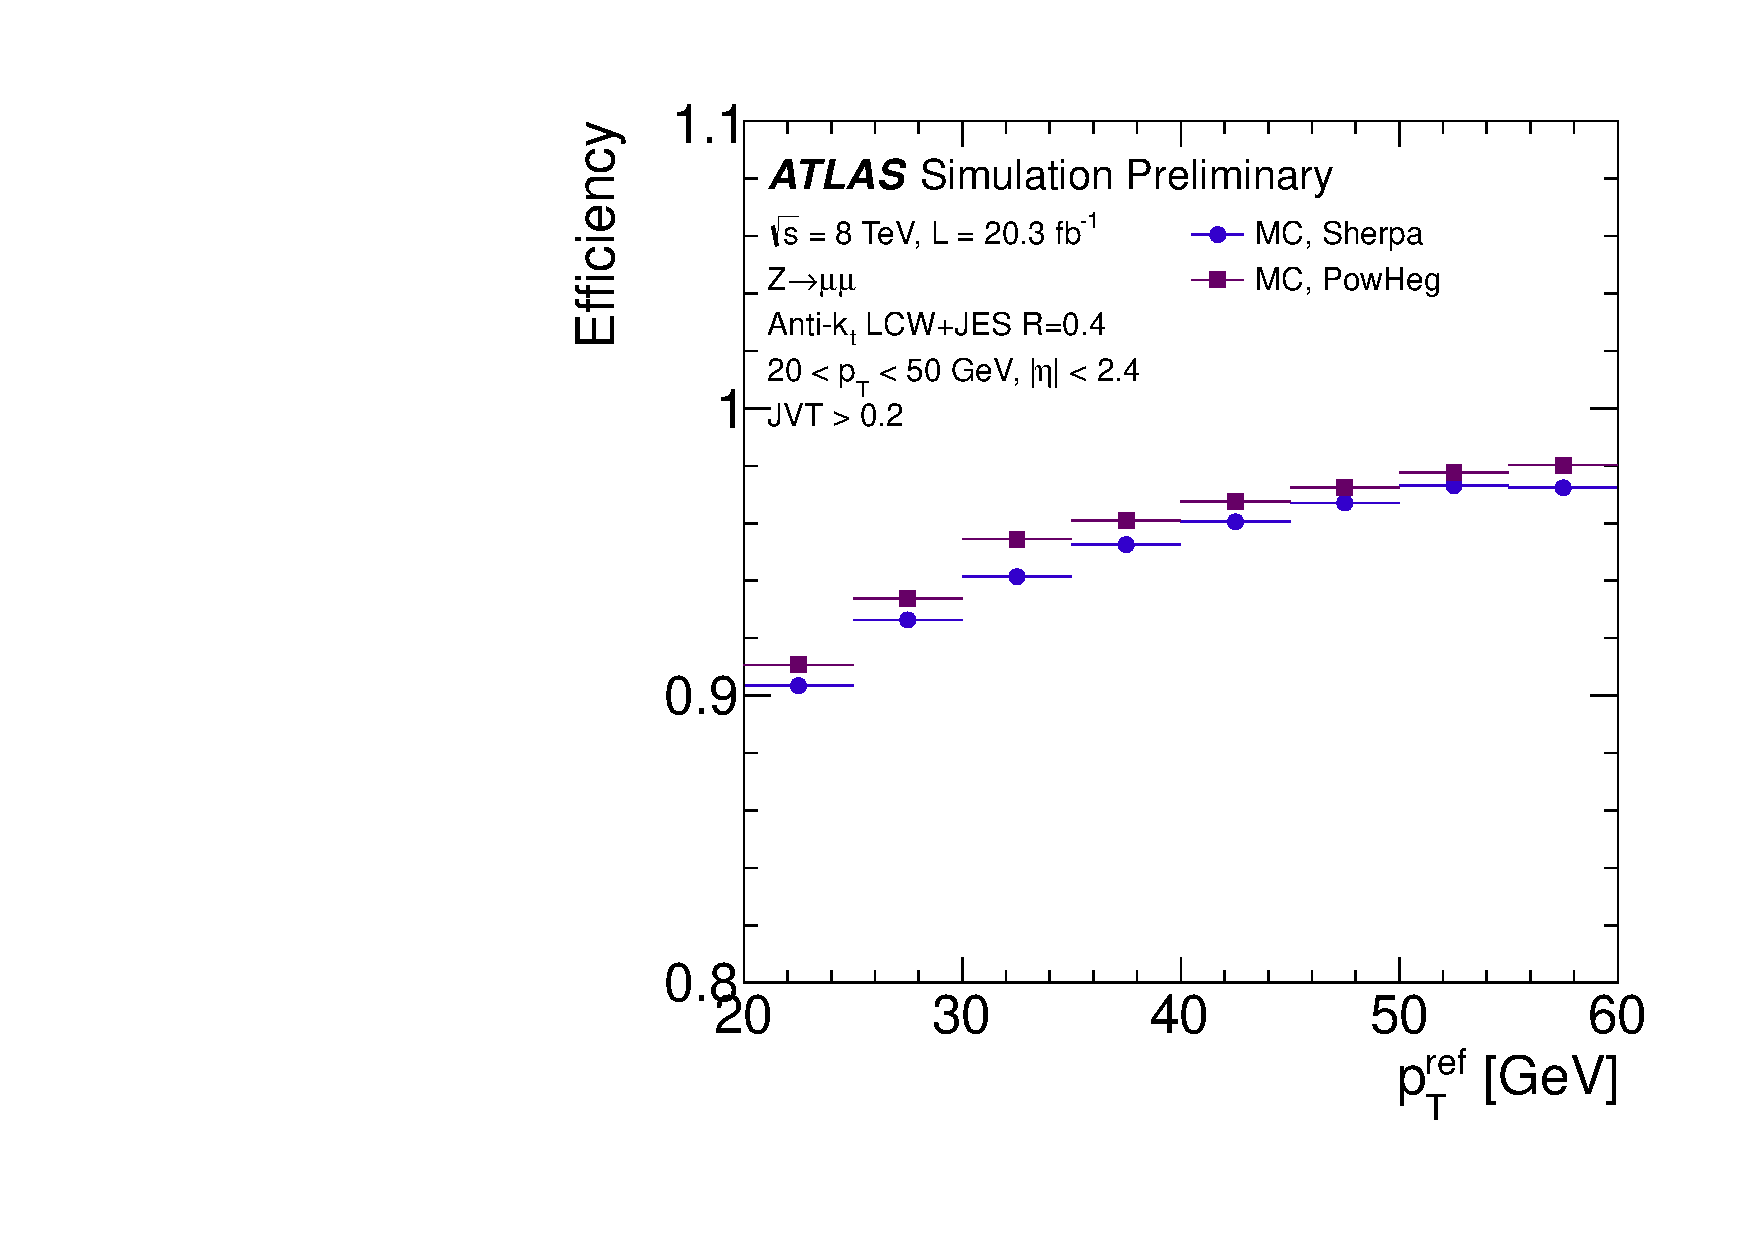
\includegraphics[width= 0.4\textwidth]{JVTEfficiency_SherpaVSPowHeg_JVTgt0p2}
  \caption{Comparison of the hard-scatter jet efficiency of a $\JVT>0.2$ requirement between the $\Zboson(\to\mu\mu)$+jets samples generated with \Sherpa and \Powheg
  as a function of $\pT^{\rm ref}$.}
  \label{fig:JVTeff_Syst}
\end{figure}
%------------------------
The total uncertainty ranges from 2\% to 1\% for $\pT^{\rm ref}$ from 20 to 60\GeV. 

%----------------------
\begin{figure}[!htbp]
  \centering
  \subfigure[]{
      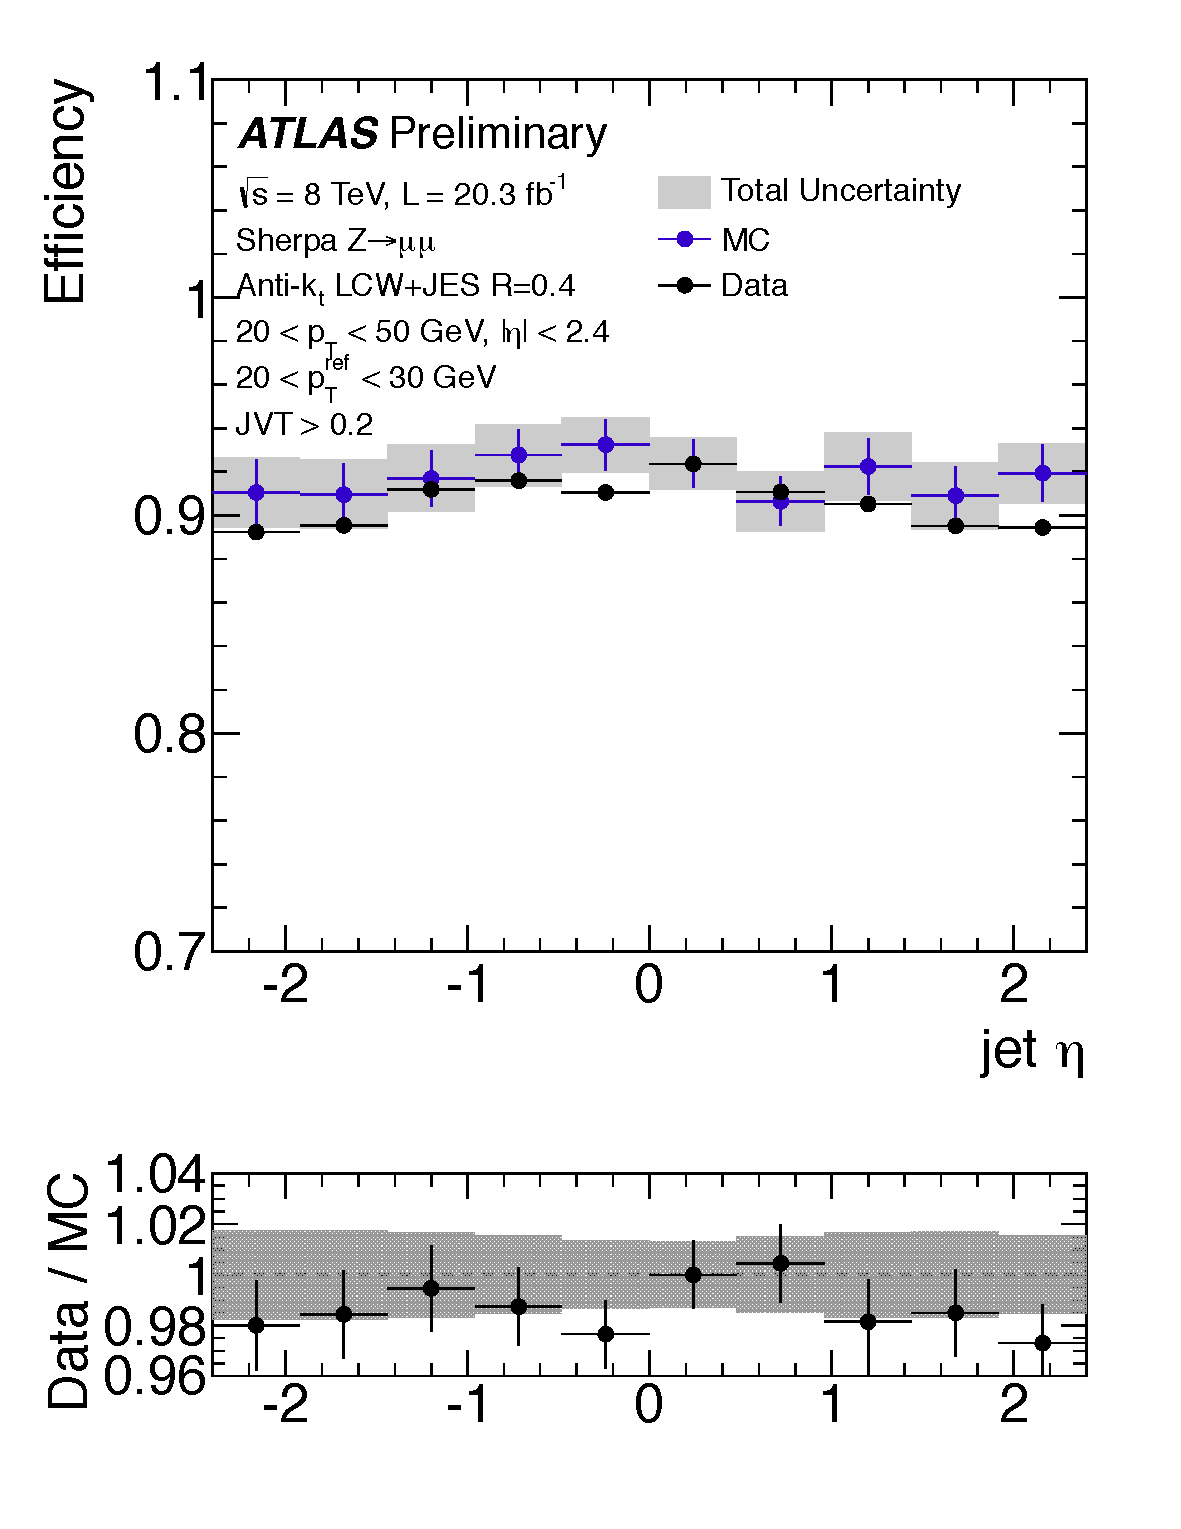
\includegraphics[width= 0.31\textwidth]{JVTCalibration_pTref_JVTgt0p2_ratio_Eta_pt20to30}
      \label{fig:JVTCal_0p2_eta_pt20to30}
  }
  \subfigure[]{
      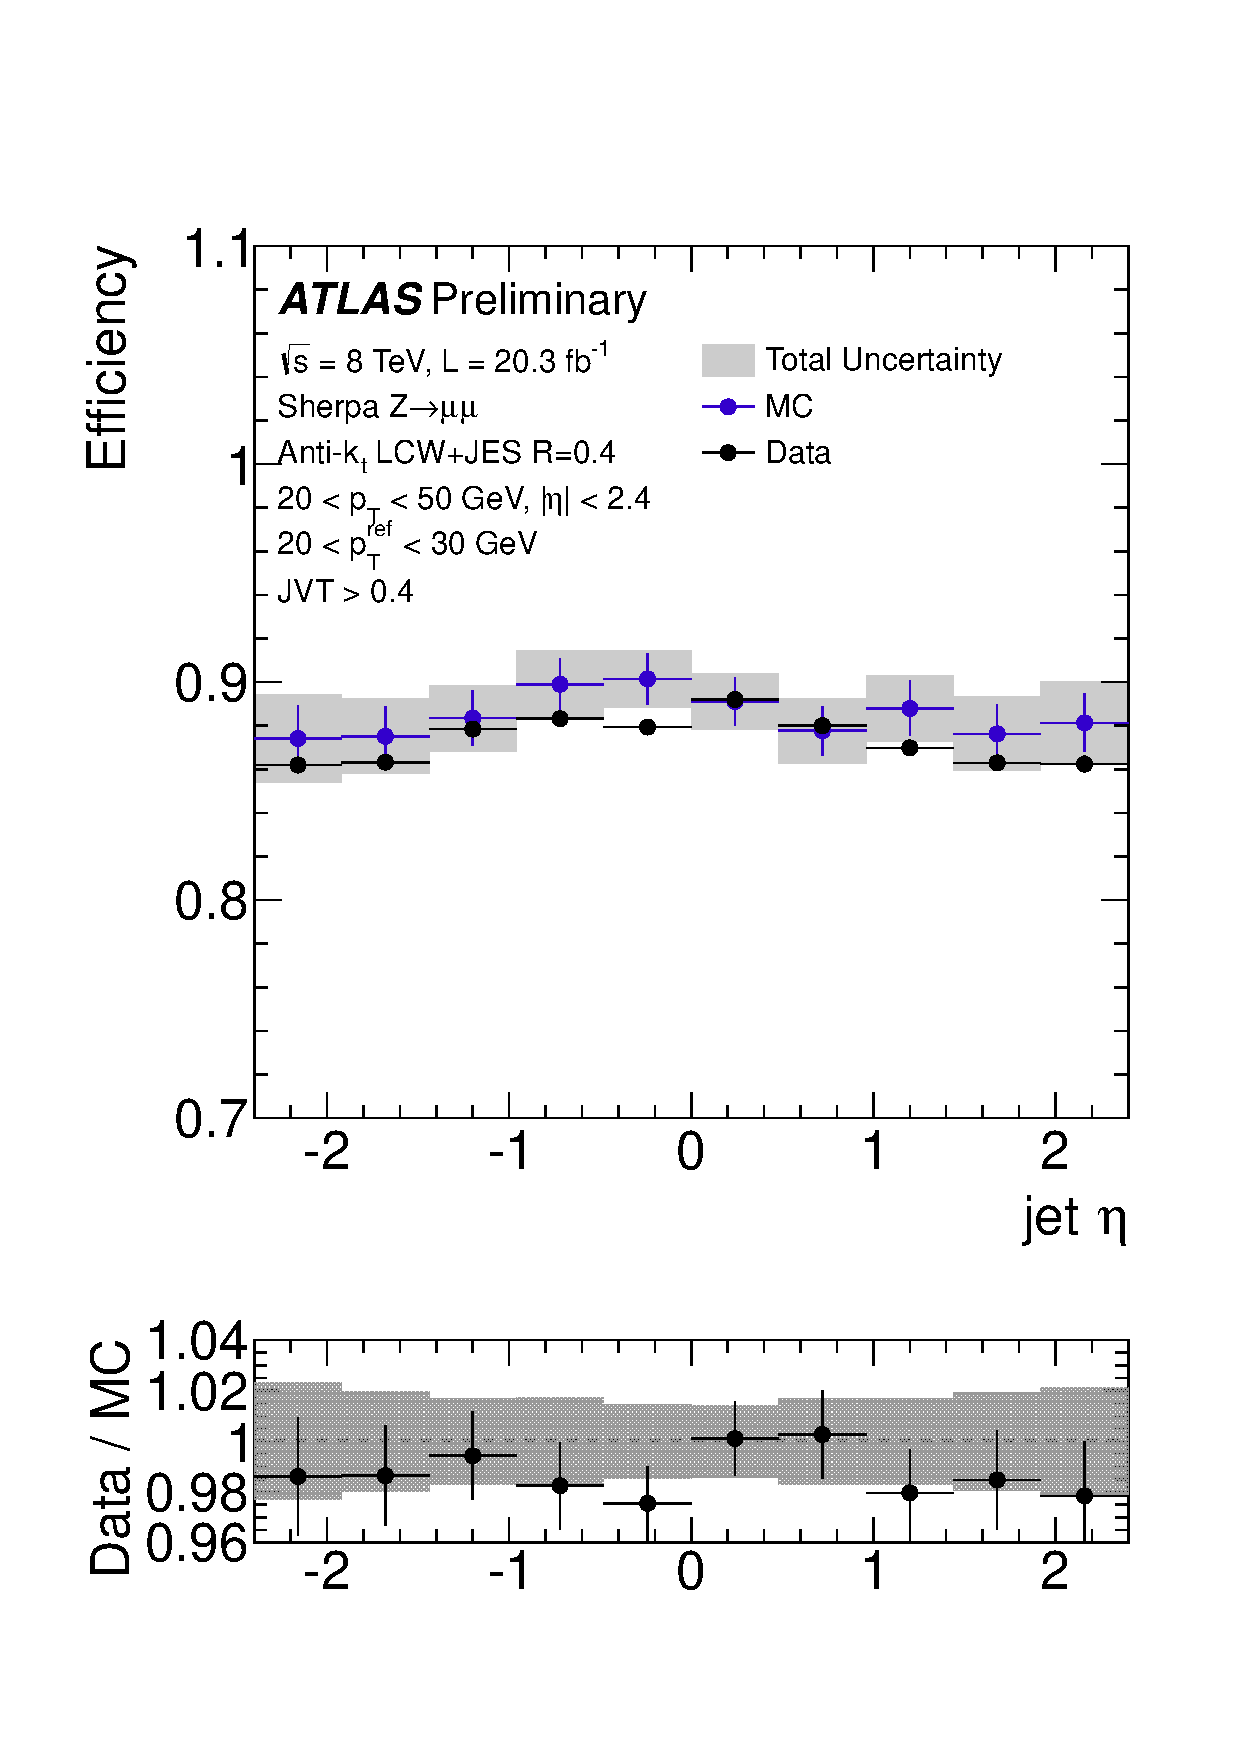
\includegraphics[width= 0.31\textwidth]{JVTCalibration_pTref_JVTgt0p4_ratio_Eta_pt20to30}
      \label{fig:JVTCal_0p4_eta_pt20to30}
  }
  \subfigure[]{
      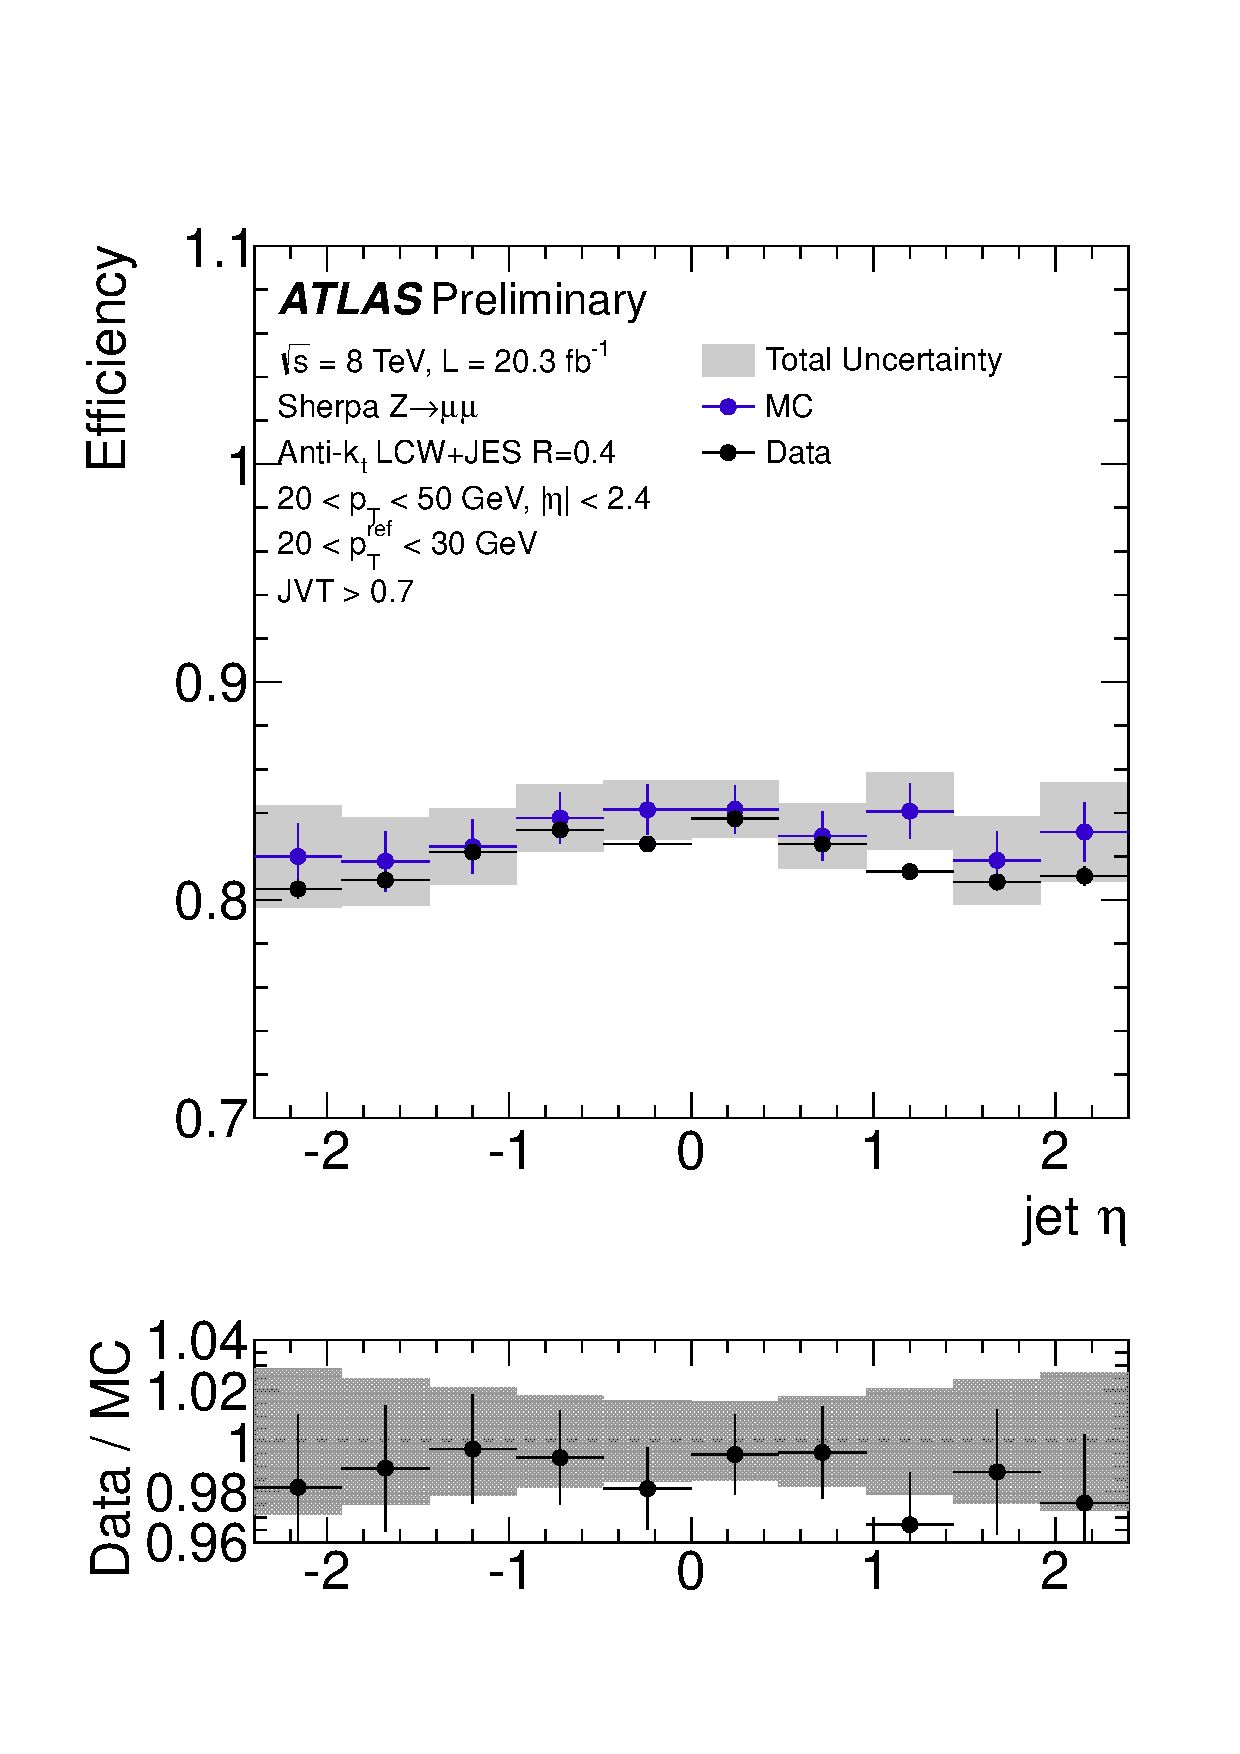
\includegraphics[width= 0.31\textwidth]{JVTCalibration_pTref_JVTgt0p7_ratio_Eta_pt20to30}
      \label{fig:JVTCal_0p7_eta_pt20to30}
  }
  \subfigure[]{
      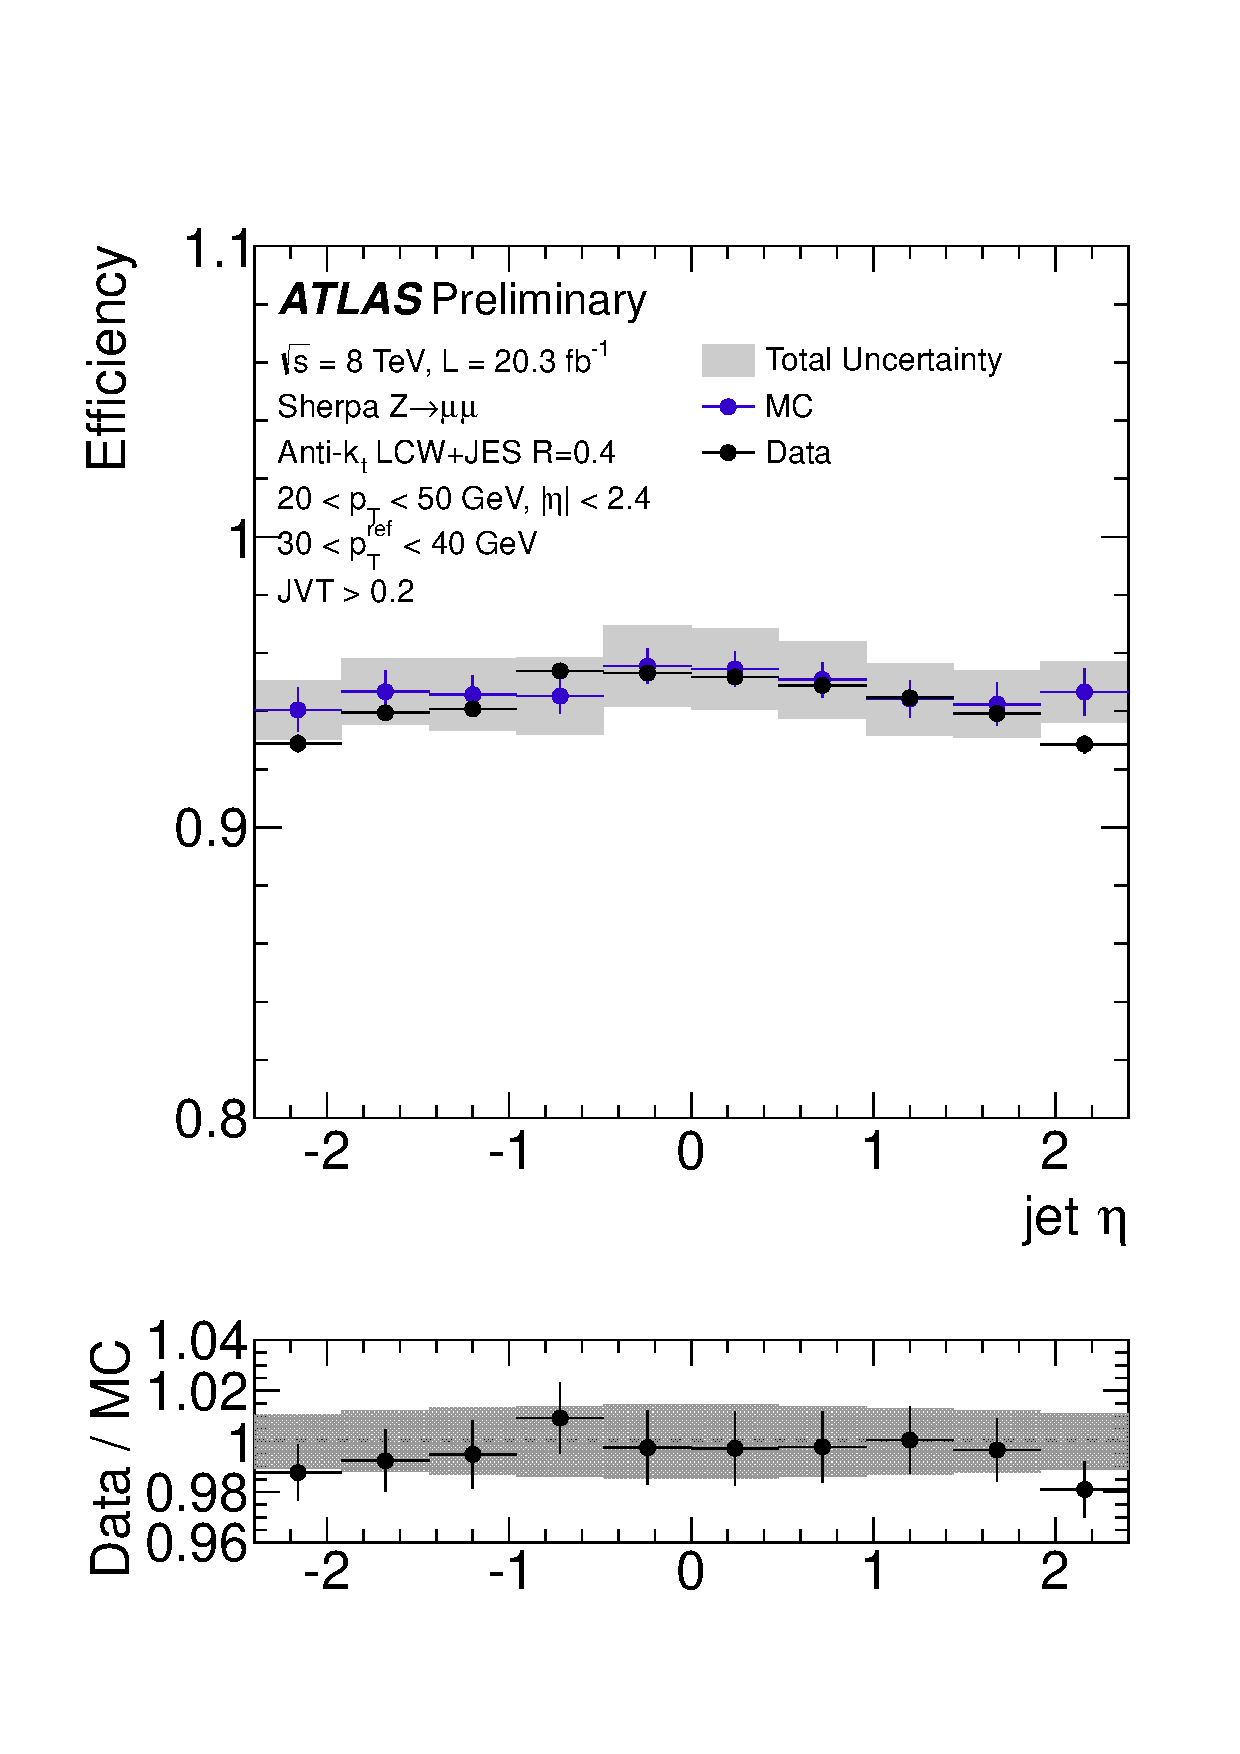
\includegraphics[width= 0.31\textwidth]{JVTCalibration_pTref_JVTgt0p2_ratio_Eta_pt30to40}
      \label{fig:JVTCal_0p2_eta}
  }
  \subfigure[]{
      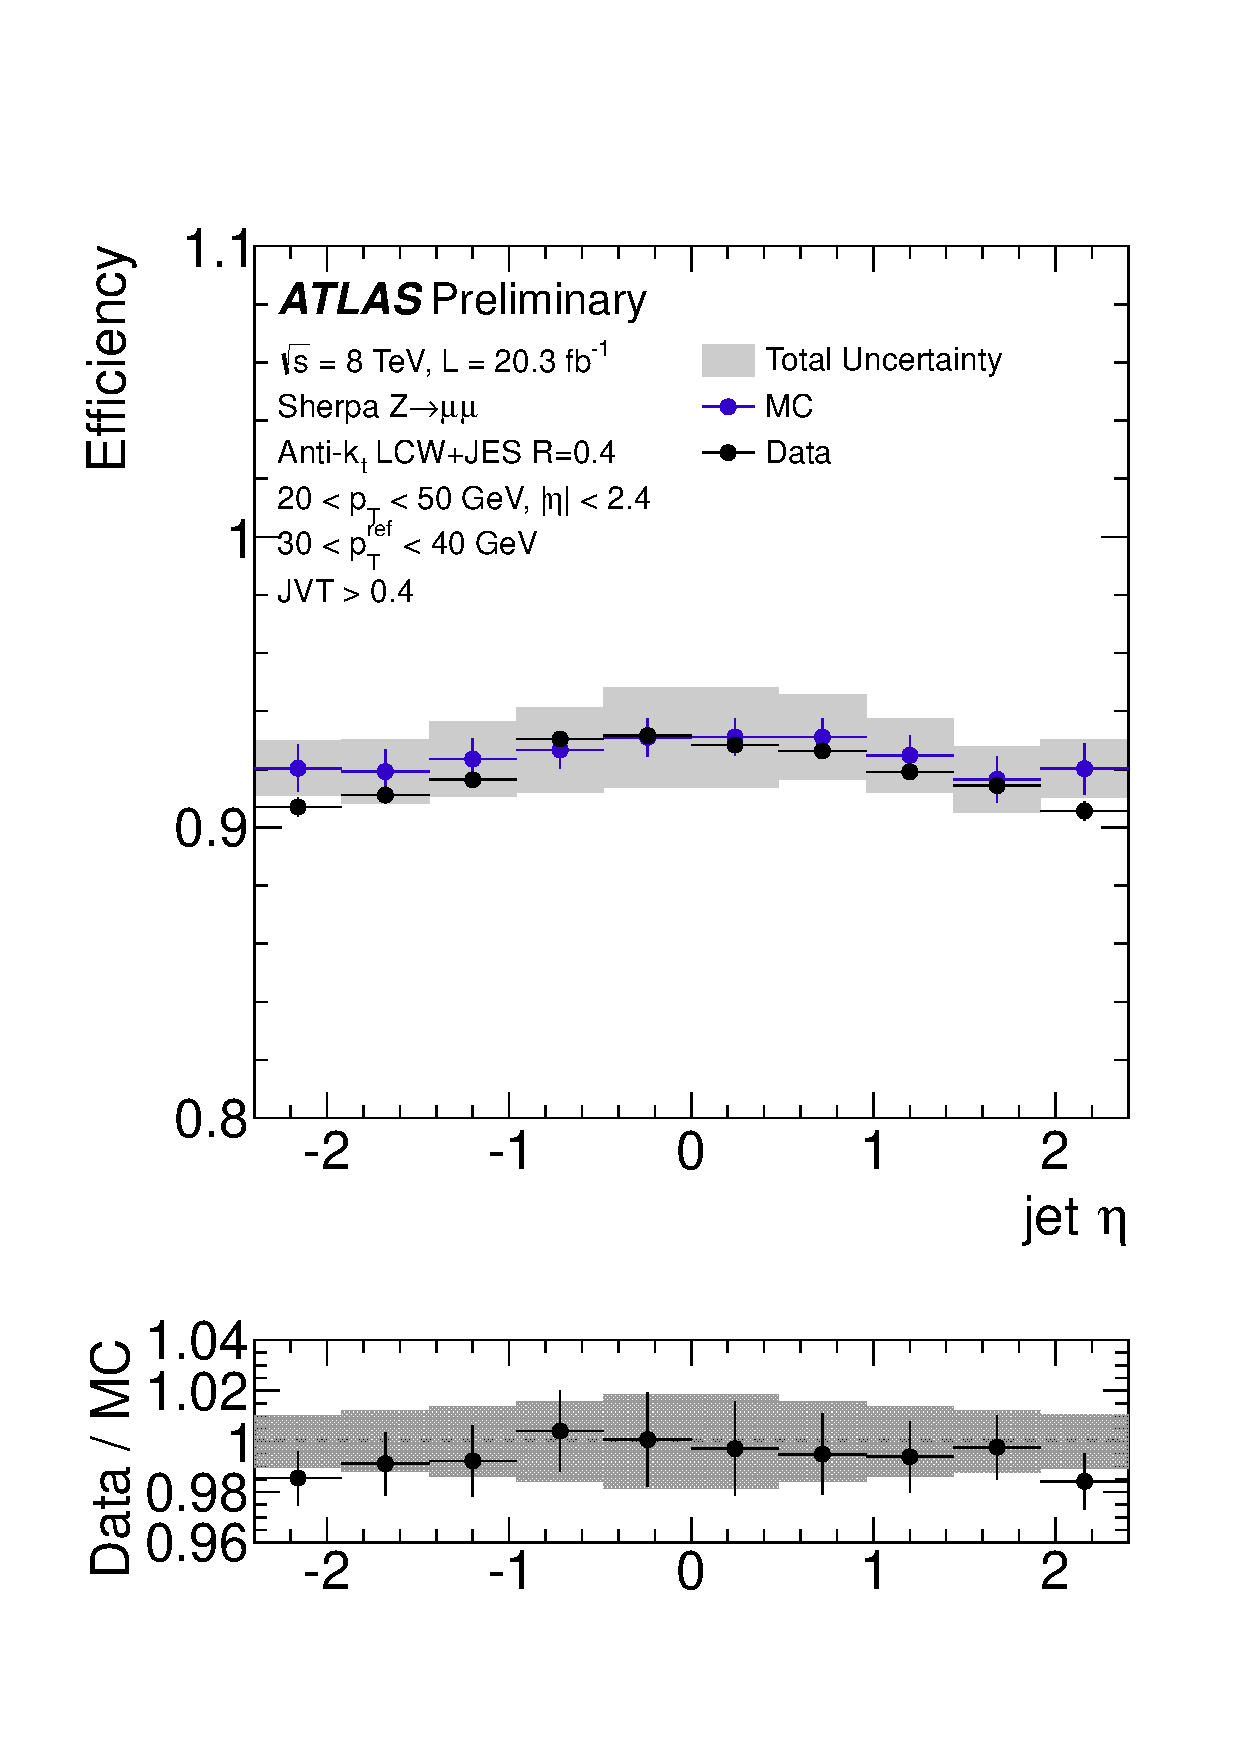
\includegraphics[width= 0.31\textwidth]{JVTCalibration_pTref_JVTgt0p4_ratio_Eta_pt30to40}
      \label{fig:JVTCal_0p4_eta}
  }
  \subfigure[]{
      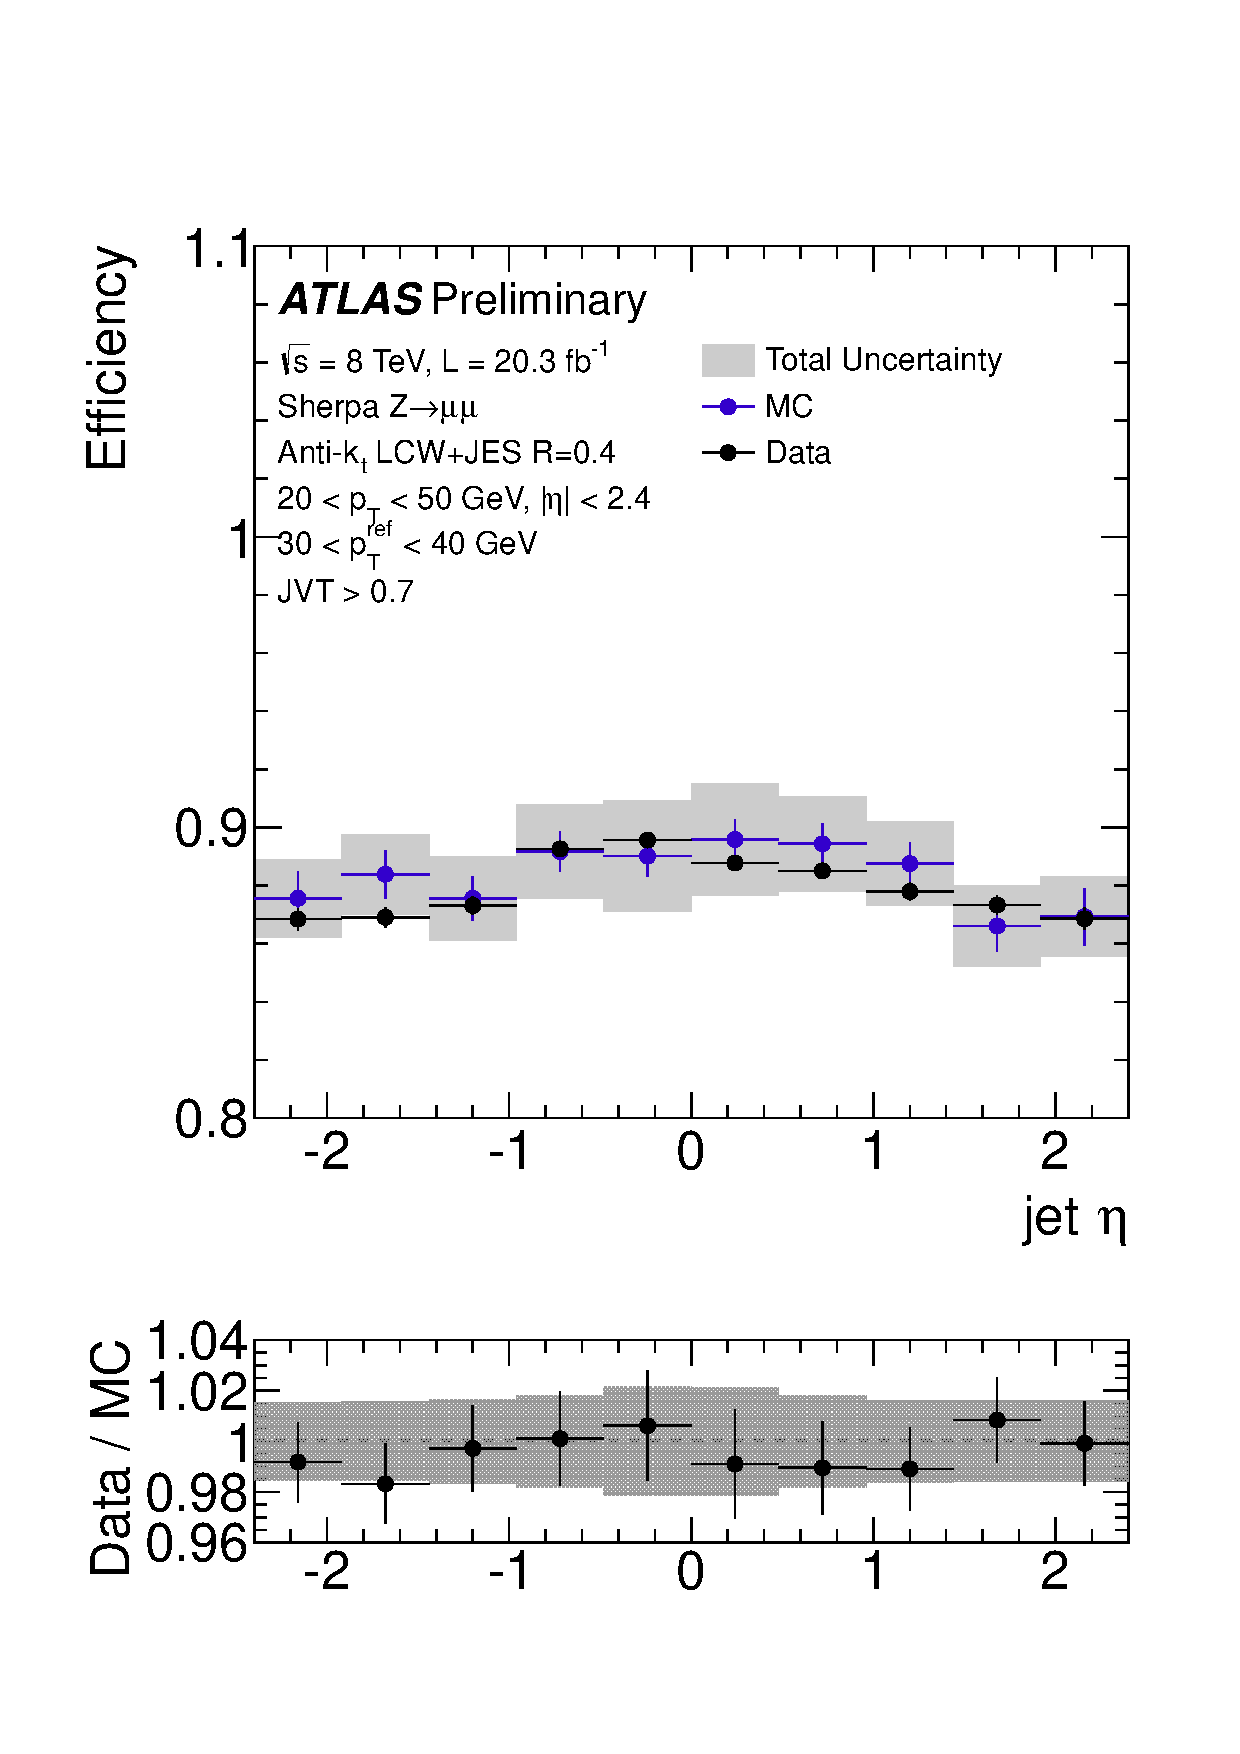
\includegraphics[width= 0.31\textwidth]{JVTCalibration_pTref_JVTgt0p7_ratio_Eta_pt30to40}
  \label{fig:JVTCal_0p7_eta}
  }
  \subfigure[]{
      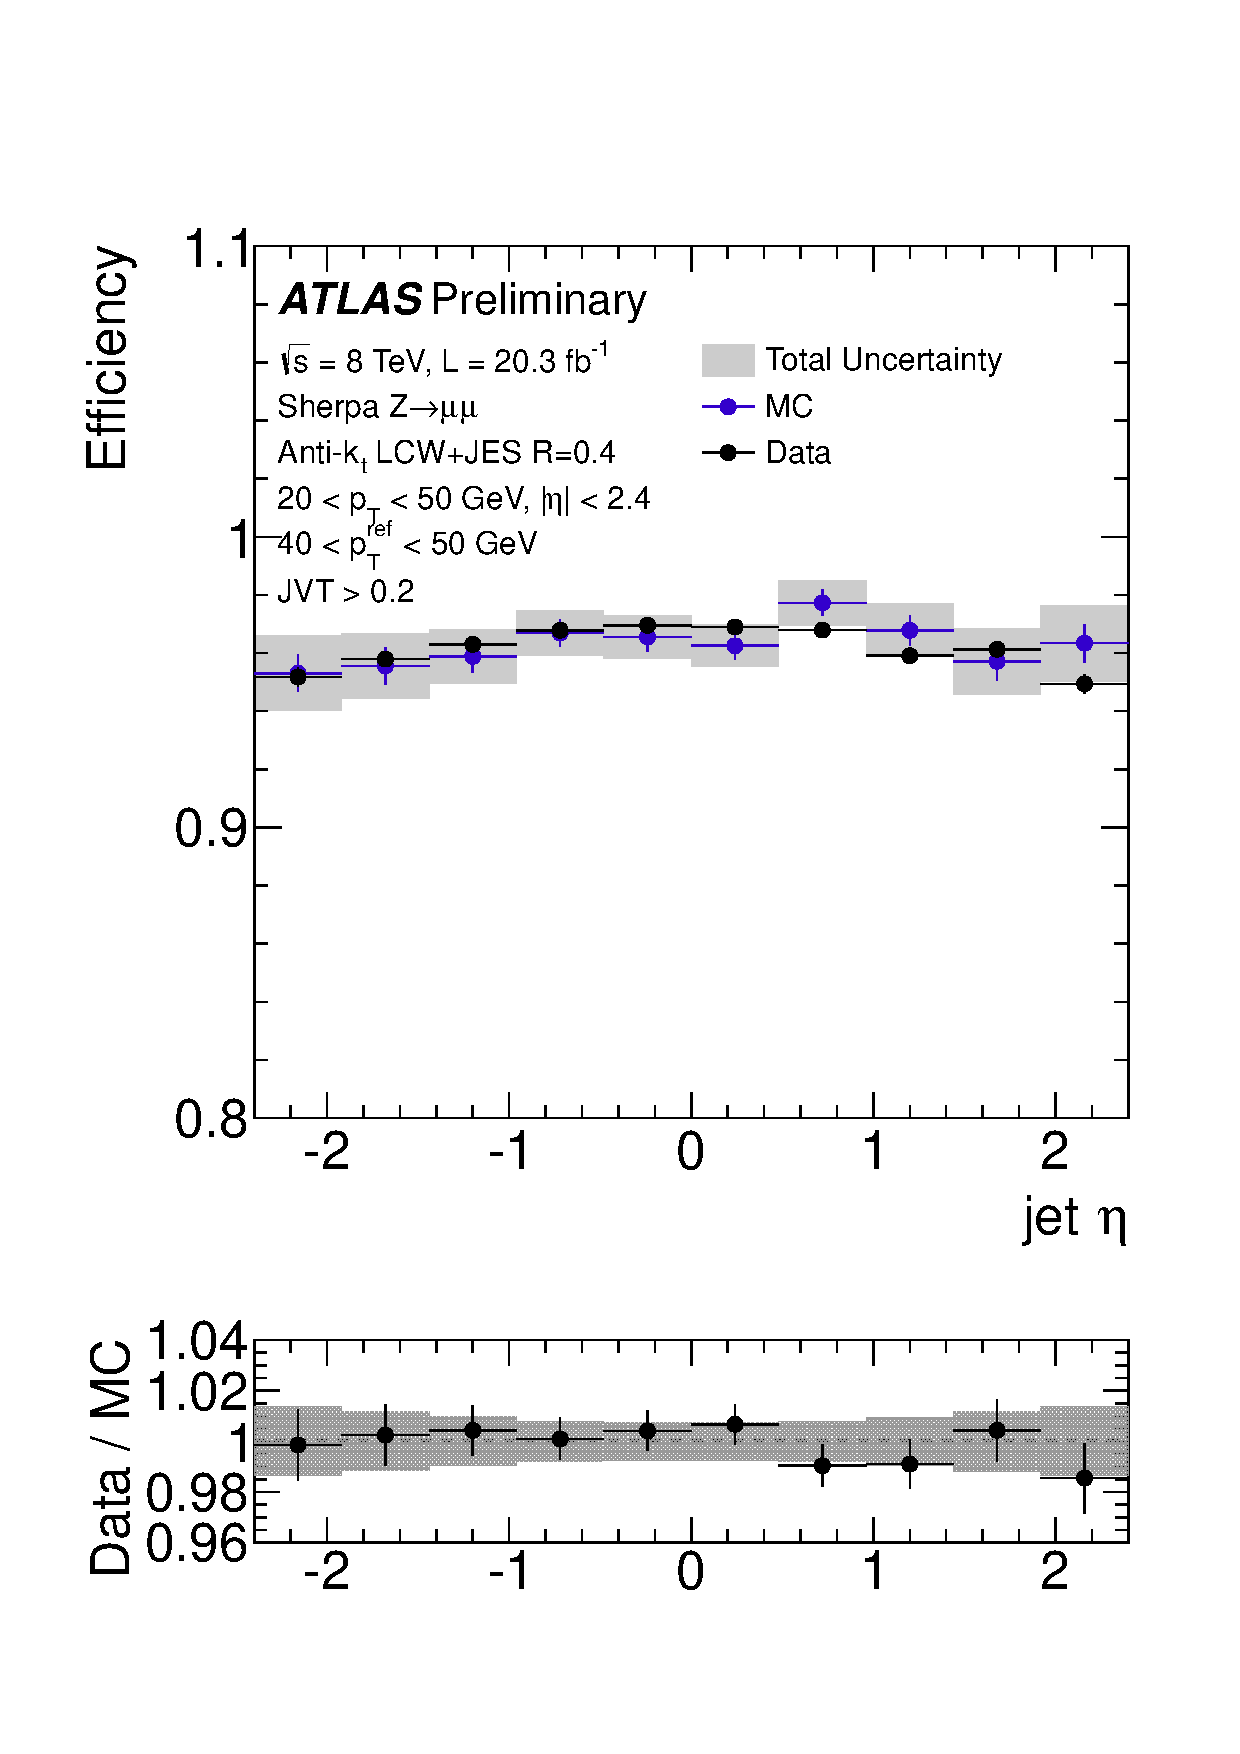
\includegraphics[width= 0.31\textwidth]{JVTCalibration_pTref_JVTgt0p2_ratio_Eta_pt40to50}
      \label{fig:JVTCal_0p2_eta_pt40to50}
  }
  \subfigure[]{
      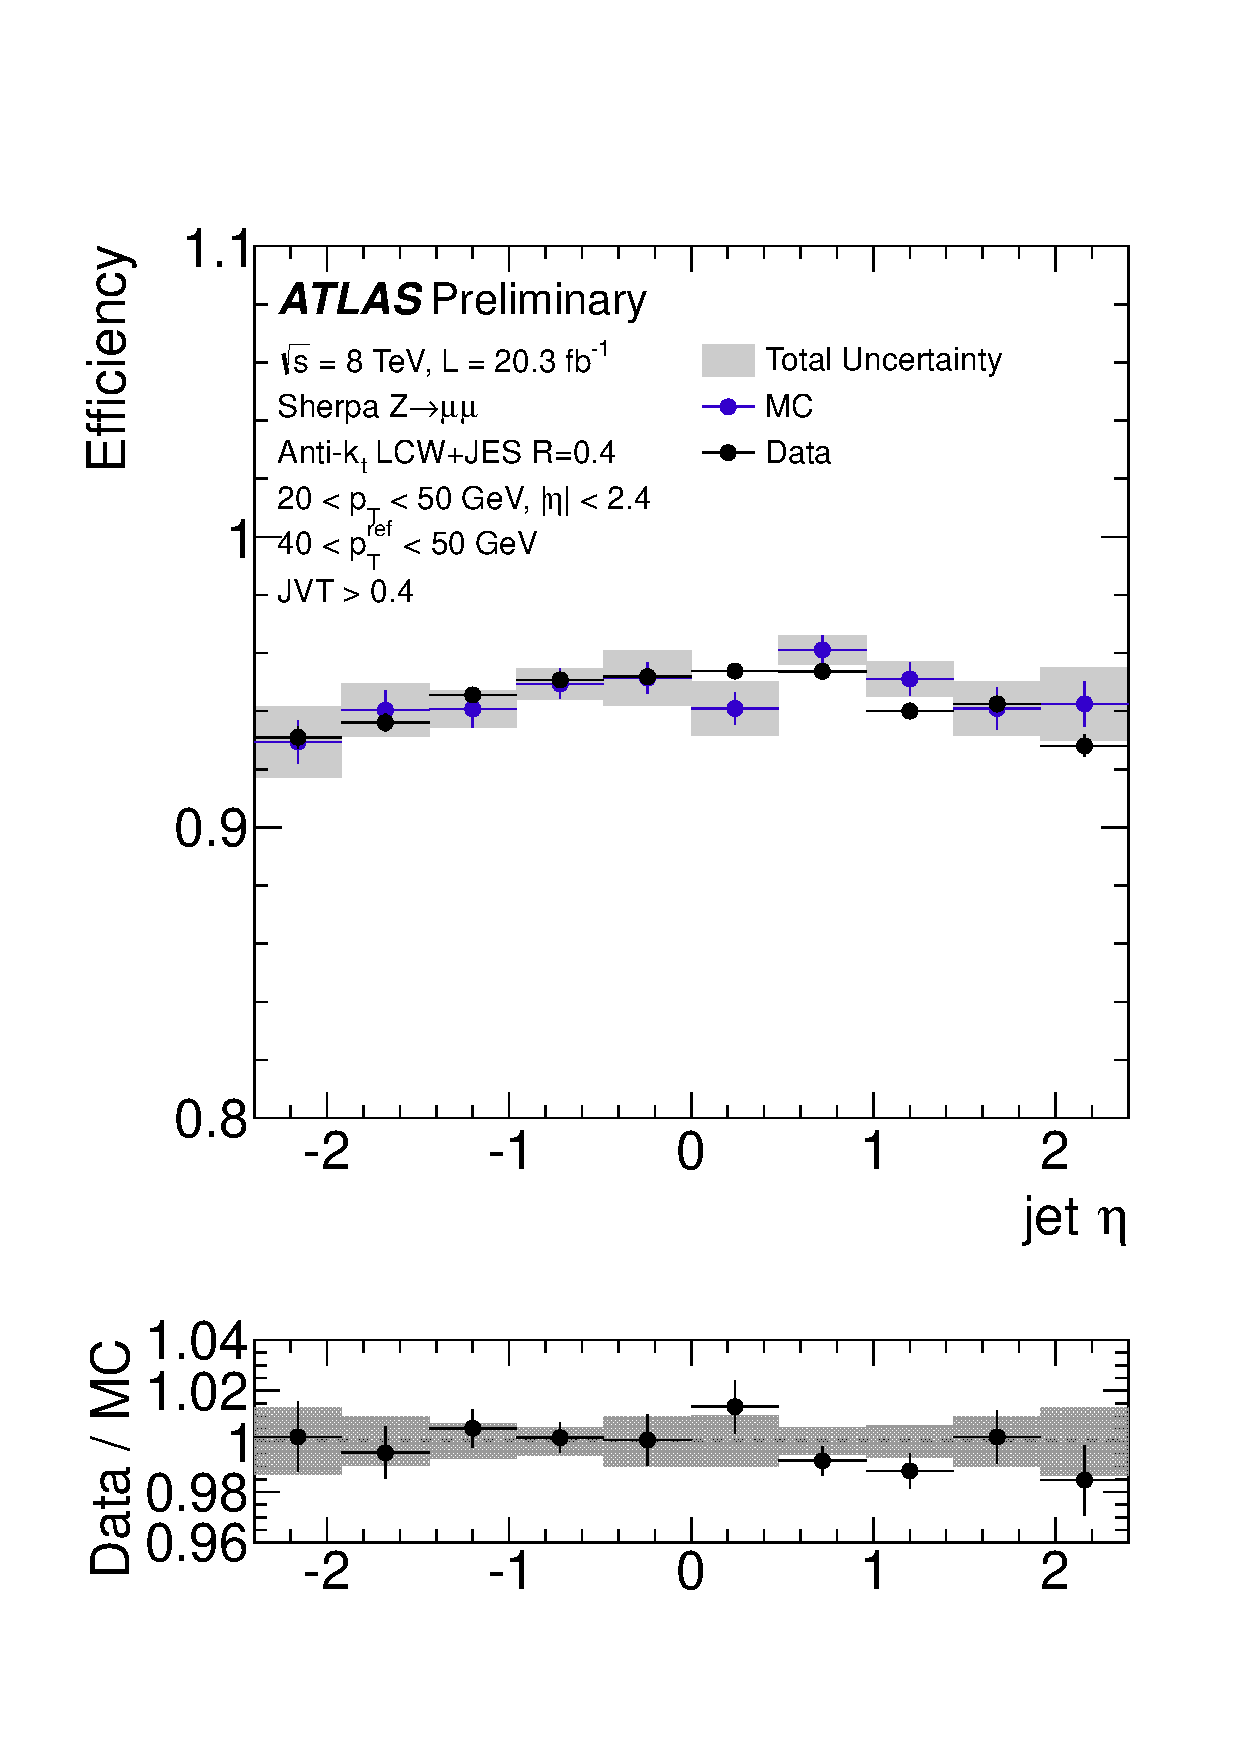
\includegraphics[width= 0.31\textwidth]{JVTCalibration_pTref_JVTgt0p4_ratio_Eta_pt40to50}
      \label{fig:JVTCal_0p4_eta_pt40to50}
  }
  \subfigure[]{
      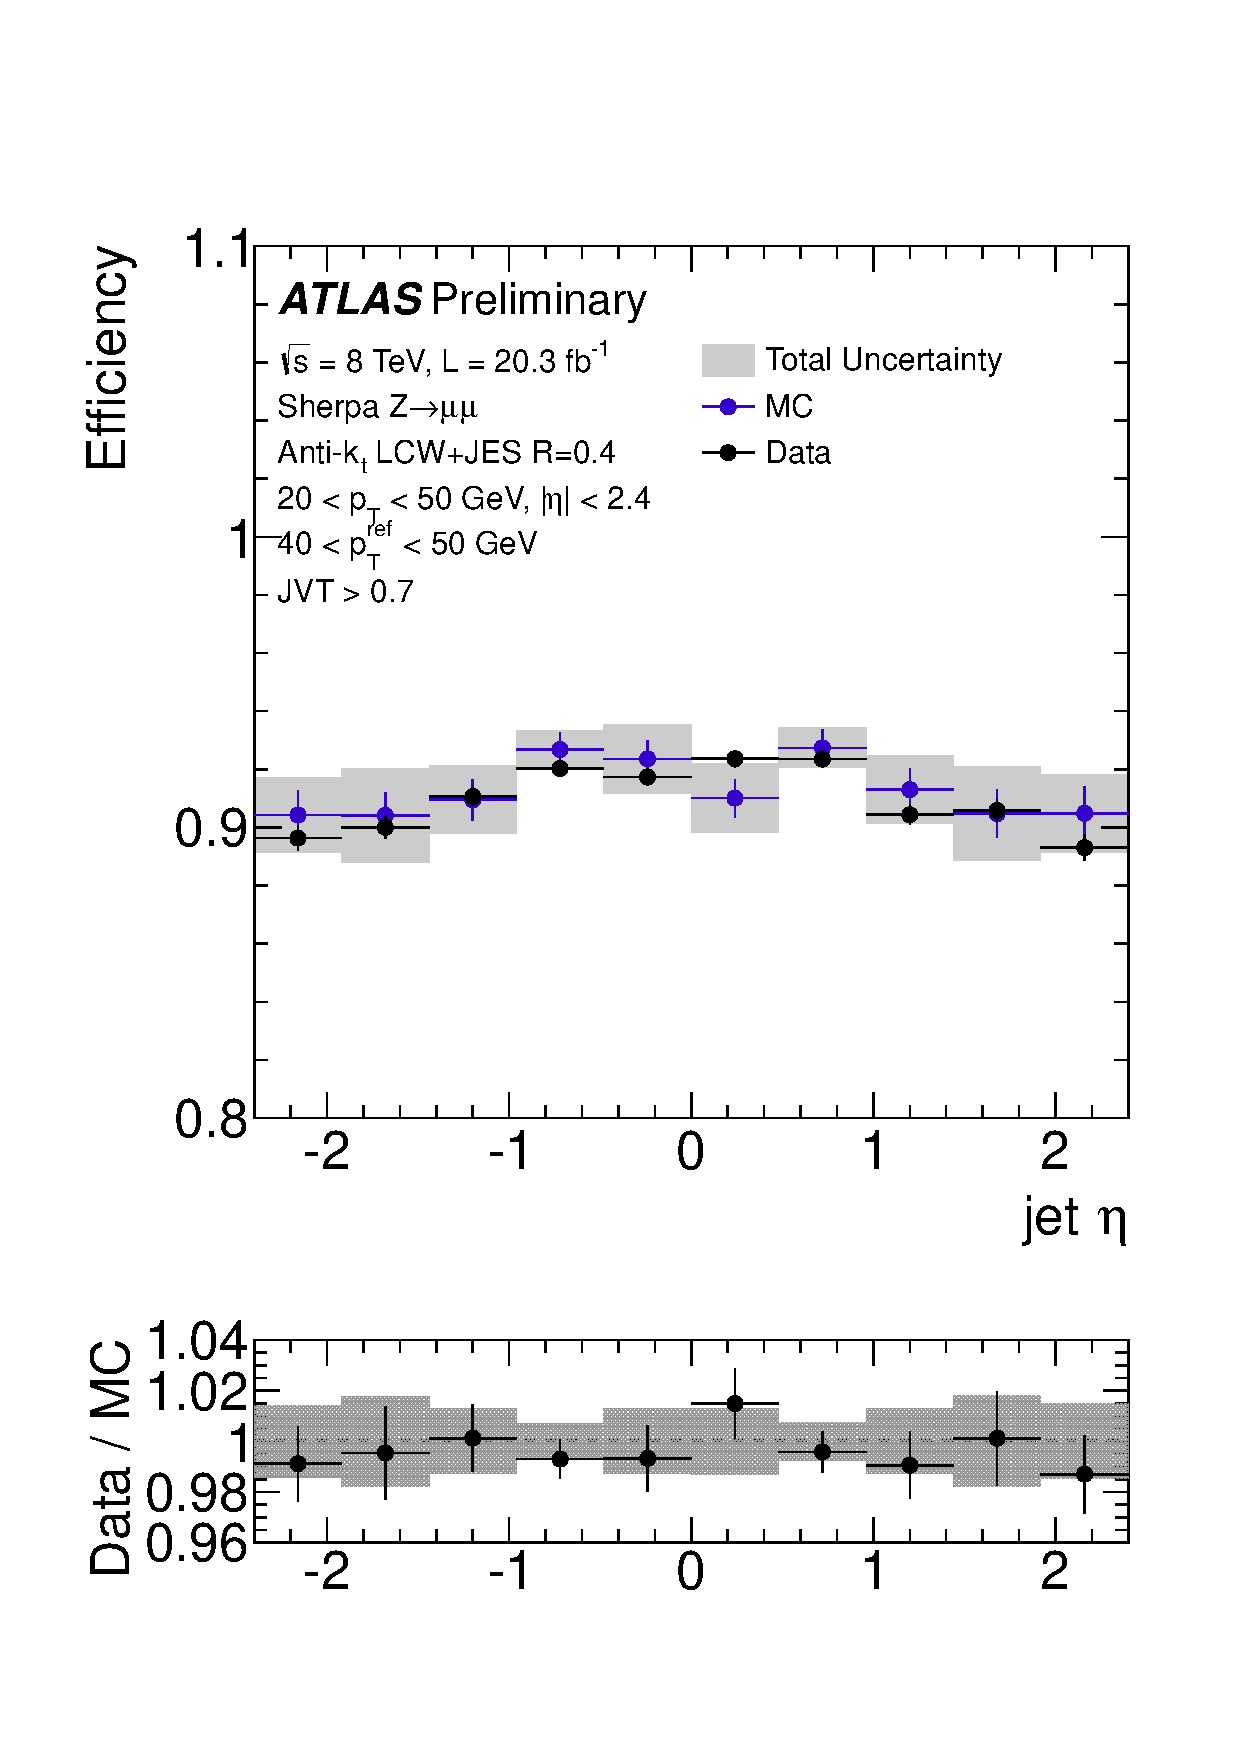
\includegraphics[width= 0.31\textwidth]{JVTCalibration_pTref_JVTgt0p7_ratio_Eta_pt40to50}
      \label{fig:JVTCal_0p7_eta_pt40to50}
  }
  \caption{Efficiency of a $\JVT>0.2$ (a, d, g), $\JVT>0.4$ (b, e, h) and $\JVT>0.7$ (c, f, i) requirement as a function of jet $\eta$. 
  The three rows represent different bins in $\pT^{\rm ref}$: $20<\pT^{\rm ref}<30 \GeV$ in (a, b, c), $30<\pT^{\rm ref}<40 \GeV$ in (d, e, f) and $40<\pT^{\rm ref}<50 \GeV$ in (g, h, i). }
  \label{fig:JVTCalibration_eta}
\end{figure}
%------------------------
Figure~\ref{fig:JVTCalibration_eta} shows the jet efficiency for minimal \JVT requirements of 0.2, 0.4 and 0.7
as a function of jet $\eta$, when selecting different slices in $\pT^{\rm ref}$. The total uncertainty on the measurement is slightly increased to due
the slicing in one more dimension. 



A $\JVT > 0.4$ ($\JVT >0.7$) requirement results in efficiencies of 86\% to 96\% (82\% to 92\%) for $\pT^{\rm ref}$ from 20 to 60\GeV. 
The looser $\JVT > 0.2$ requirement is about 90\% efficient for $\pT = 20 \GeV$ jets, reaches an efficiency of at least $96\%$ for jets with $\pT > 40\GeV$, and is thus
preferable in a multi-jet environment to avoid significant efficiency losses. 
It should be noted that these numbers correspond to efficiencies for jets failing the pileup jet definition, 
which are not necessarily
hard-scatter jets as defined in Section~\ref{sec:jets} since a few percent of jets in the signal region are classified as neither hard-scatter nor pileup jets. 
In simulation, the jet efficiency of a $\JVT > 0.2,0.4,0.7$ requirements are about 1--2\% higher when only using truth-matched hard-scatter jets. 


%--------------------------------------------------------------------------------------------------
\section{Applications of \JVT-based pileup jet suppression}
\label{sec:JVTapplication}
\subsection{Jet multiplicity in $\Zboson(\to\mu\mu)$+jets events}
%-------------------------------------
\begin{figure}[!htbp]
 \centering
 \subfigure[]{
     \includegraphics[width= 0.46\textwidth]{JetMult_Zmumu}
     \label{fig:JetMultZmumu}
 }
 \subfigure[]{
     \includegraphics[width= 0.46\textwidth]{JetMultSlope_Zmumu}
     \label{fig:JetMultSlopeZmumu}
 }
 \caption{(a) The jet multiplicity $\langle N_{j}\rangle$ for jets with $\pT>20\GeV$ and $|\eta|<2.4$ as a function of the average number of interactions per bunch crossing $\mu$ in $\Zboson(\to\mu\mu)$+jets events. 
          (b) The change in the jet multiplicity with $\mu$ as a function of $\mu$ for the same event selection. $\langle N_{j}\rangle$ increases with $\mu$ at a $\mu$ dependent rate that 
          is different for data and simulation. After imposing a $\JVT>0.7$ requirement, the number of jets is observed to be independent of $\mu$.
 }
 \label{fig:JetMult}
\end{figure}
Figure~\ref{fig:JetMultZmumu} shows the average jet multiplicity $\langle N_{j}\rangle$ as 
a function of the average number of pp interactions per bunch crossing $\mu$ for $\Zboson(\to\mu\mu)$+jets events in data and simulation. 
When no selection criteria are applied to suppress pileup jets, the mean number of jets per event increases with $\mu$ at a rate that is different between data and simulation. 
However, the jet multiplicity is stable and independent of $\mu$ after imposing a $\JVT>0.7$ criterion. 
% For this selection of jets, the $\JVT > 0.7$ 
% requirement corresponds to a hard-scatter jet efficiency of about $90\%$. 
Figure~\ref{fig:JetMultSlopeZmumu} shows the change in the jet multiplicity $(\langle N_j \rangle)$ 
with $\mu$ as a function of $\mu$ using the same selection of $\Zboson(\to\mu\mu)$+jets events. The slope is calculated from the difference in $\langle N_j \rangle$ between adjacent bins.
When no pileup suppression criteria are applied, 
the graphs follow an approximately linear trend, indicating a quadratic increase in the jet multiplicity with $\mu$. After imposing a $\JVT>0.7$ criterion, 
no significant change in the jet multiplicity is observed with $\mu$ for the full range of $\mu$ both for data and simulation.

%------------------------------
\subsection{Jet veto efficiency in VBF ${\rm H} \to 4\ell$ events}
%-------------------------------------
\begin{figure}[!htbp]
 \centering
 \subfigure[]{
     \includegraphics[width= 0.46\textwidth]{VBF_H_JetVetoEff}
     \label{fig:VBF_Higgs_0p7}
 }
 \subfigure[]{
     \includegraphics[width= 0.46\textwidth]{VBF_H_JetVetoEff_JVT0p2}
     \label{fig:VBF_Higgs_0p2}
 }
 \caption{Event-by-event jet-veto efficiency in VBF ${\rm H} \to 4\ell$ events as a function of \NPV and jet \pT threshold before and after a $\JVT>0.7$ (a) or $\JVT>0.2$ (b) criterion has been applied.}
 \label{fig:VBF_Higgs}
\end{figure}
%------------------------------
We use a sample of simulated $\pq \pq^{\prime} \to \Higgs \pq \pq^{\prime}$, $\Higgs \to \Zboson\Zboson \to 4 \ell$, $\ell = {\rm e},\mu$, events where the Higgs boson \Higgs is produced in vector-boson fusion (VBF)
to test the \JVT-based pileup jet suppression for an important physics analysis
that is sensitive to pileup. We adopt a similar event selection as in Ref.~\cite{ATLAS-CONF-2013-013} 
and require the two leading jets with $\pT > 20 \GeV$ to be separated in $\eta$ by more than 3 units. We use generator truth information to reject jets that overlap
within $\Delta R<0.4$ with the four leptonic decay products of the Higgs boson and require the two leading jets to originate from the selected hard-scatter vertex.
The jet-veto efficiency, defined as the fraction of events in which there is no additional jet within the tracker coverage, is
evaluated before and after a $\JVT>0.7$ ($\JVF >0.2$) criterion has been used to reject pileup jets. This efficiency is shown in Figure~\ref{fig:VBF_Higgs} 
as a function of jet \pT threshold and \NPV. If no pileup jet suppression is applied, the jet-veto efficiency is found to decrease from 80\% to 40\% and from 92\% to 88\% for 
jet veto \pT threholds of 20 and 30\GeV, respectively, for increasing \NPV from 0 to 30. This decrease is attributed to additional jets originating from pileup interactions. 
When applying a $\JVT > 0.7$ criterion, the jet-veto efficiency is stable at $85\pm2\%$ and $94\pm2\%$ for the same \pT thresholds. 
Using the looser $\JVT > 0.2$ criterion, a marginal \NPV dependence in the jet-veto efficiency is still observed when using the 20\GeV \pT threshold. 
% When only counting truth jets from the hard-scatter, 
% the jet-veto efficiencies are 90\% and 95\% for \pT thresholds of 20 and 30\GeV. 



%----------------------------------------------------------------------
\section{Track-based Grooming of Large-$R$ jets}
\label{sec:grooming}
%--------------------------

At the LHC, many interesting signatures of both Standard Model and new physics processes contain  boosted heavy particles, such 
as \Wboson, \Zboson, and \Higgs bosons, or top quarks. The successful identification of such topologies requires the use of large-$R$ jets and jet 
substructure techniques. One of the key ingredients of jet substructure studies is the use of {\it grooming} techniques 
({\it filtering}~\cite{Butterworth:2008iy}, {\it pruning}~\cite{Ellis:2009su,Ellis:2009me}, and {\it trimming}~\cite{Trimming}) that mitigate
the effect of pileup on large-$R$ jets. Since pileup effects on the jet \pT are proportional to the area of jets, grooming becomes essential 
in the case of large-$R$ ($R > 0.6$) jets. 

Jet grooming techniques attempt to identify and reject components of large-$R$ jets that are consistent with pileup depositions, effectively 
reducing the jet area and the sensitivity to pileup. In the case of trimming, for example, $R=0.3$ $k_t$ subjets with a \pT fraction relative
to the parent (ungroomed) jet smaller than $f_{\rm cut} = p^{subjet}_T/p^{jet}_T = 0.05$ are removed. 

Building upon the success of calorimeter-based grooming methods and track-based pileup suppression of small-$R$ jets, 
a new, track-based, grooming technique can be designed by applying \cJVF to the individual subjets of large-$R$ jets. In particular, track-based
trimming can be implemented by replacing the $f_{\rm cut}$ criterion with a requirement on the \cJVF of subjets. Other variables,
such as \JVT or \RpT can also be considered, but this note focuses on the use of \cJVF as an example of a purely track-based 
grooming procedure. 

In order to illustrate the concept of track-based grooming, it is useful to consider an event display. Figure~\ref{fig:EventDisp} 
%--------------------------
\begin{figure}[!htbp]
  \centering
  \subfigure[]{
      \includegraphics[width= 0.48\textwidth]{EventDisplay_16552_Full_Preliminary}
    \label{fig:EventDisplay1}
  }
  \subfigure[]{
      \includegraphics[width=0.48\textwidth]{EventDisplay_16552_zoom_Preliminary}
    \label{fig:EventDisplay2}
  }
  \caption{(a) Rapidity - $\phi$ view of a simulated event of a $\Wboson^{\prime}$ boson with a mass of 1\TeV decaying to a \Wboson 
and a \Zboson. (b) Zoom-in version of (a).}
\label{fig:EventDisp}
\end{figure}
%------------------------
shows the rapidity $y$ vs.~azimuthal angle $\phi$ view of a simulated event where a $\Wboson^{\prime}$ boson with a mass of 1\TeV decays to a \Wboson and a \Zboson boson, 
which decay hadronically. The orange star and blue triangle indicate the $y$ - $\phi$ 
positions of the generated \Zboson and \Wboson bosons. The large circles represent the active area boundaries of 
the anti-$k_{t}$ $R=1.0$ jets, built from topological calorimeter clusters~\cite{Lampl:1099735}. 
In the following, these jets are referred to as ungroomed jets. The clusters are represented by small solid squares with colors ranging from blue to red encoding low to high transverse energies. 
The gray regions indicate the active areas of the $k_t$ $R=0.3$ subjets 
reconstructed from the constituents of the ungroomed jets. Only subjets with a \pT of at least $5\%$ of the ungroomed jet \pT are shown. 
Tracks associated with the jet and originating from the hard-scatter vertex (black open circles) or from pileup vertices (black crosses) 
are also indicated. The violet ungroomed jet (with $\phi \approx 4.1$ and $y \approx -0.2$) has a \pT of 446\GeV and is matched in $\Delta R$ to the truth \Zboson boson. 
While all three subjets have active areas overlapping with the $y-\phi$ positions of pileup tracks, only two subjets have 
associated hard-scatter tracks. 
The invariant mass reconstructed from the two subjets with hard-scatter tracks is 89\GeV and the one from all three subjets is 119\GeV.
This event display shows that tracking information can provide complementary information to calorimeter-based trimming. 
Track-assisted trimming would allow the rejection of the third subjet, which is likely to originate from pileup, while keeping the two subjets from the \Zboson boson. 

%------------------------
\begin{figure}[!htbp]
  \centering
  \includegraphics[width= 0.6\textwidth]{TrackBasedTrimming_CorrJVF_vs_pTratio_fCutline}
  \caption{Correlation of subjet \pT fraction and subjet \cJVF for anti-$k_t$ $R=1.0$ jets with $\pT>300\GeV$ and $|\eta| <1.5$. 
The dotted line indicates the standard calorimeter-based trimming \pT ratio cut of $5\%$. Calorimeter-based trimming would remove all subjets
that are below the dotted line, including those with large \cJVF values at the lower right.}
  \label{fig:TrackBasedTrimming_Correlation}
\end{figure}
%------------------------
Figure~\ref{fig:TrackBasedTrimming_Correlation} shows the ratio of the subjet \pT and the ungroomed jet \pT 
on a log-scale as a function of the subjet \cJVF in simulated $\Wboson^{\prime} \to \Wboson \Zboson \to \pq\pq\pq\pq$ events. 
The 2-dimensional distribution is normalized to unit area. About 4\% of subjets that have no associated tracks ($\cJVF=-1$) are omitted. 
Ungroomed jets are selected that have a \pT of at least 300\GeV, $|\eta| <1.5$, and are matched in $\Delta R$ to the truth \Zboson. 
The \cJVF of the subjets is calculated from the associated hard-scatter and pileup tracks. Most subjets with significant \pT ratio 
also have large \cJVF, 
indicating that most of their charged \pT comes from the hard-scatter vertex. A large fraction of subjets with a low \pT 
ratio $< 5\%$ $(\log_{10}[\pT^{\rm sub}/\pT^{\rm ungroomed}] <-1.3)$ and a few subjets with a significant \pT ratio, 
however, have small \cJVF values. Most such subjets are consistent with pileup and should be excluded in a track-based jet grooming procedure. 
Similarly, subjets with small \pT ratio and large \cJVF that would be removed by calorimeter-based trimming, should be kept by the track-based 
trimming algorithm. 

%--------------------------
\begin{figure}[!htbp]
  \centering
  \subfigure[]{
      \includegraphics[width= 0.46\textwidth]{TrackBasedTrimming_corrJVF}
    \label{fig:TrackBasedTrimming_cJVF_differentFCut}
  }
  \subfigure[]{
      \includegraphics[width=0.46\textwidth]{TrackBasedTrimming_comparison}
    \label{fig:TrackBasedTrimming_comparison}
  }
  \caption{Distribution of the mass of the jet matched to the truth \Zboson boson for different trimming configurations based on \cJVF and $f_{\rm cut}$. 
The blue shaded histogram shows the ungroomed jet mass. (a) In the histograms with magenta, blue and green markers, 
the groomed jet mass is computed from subjets that satisfy 
a $\cJVF > 0.6$ requirement, \ie excluding subjets from pileup interactions. 
In the blue and green histograms, the subjets are further required to have $\pT^{\rm subj} / \pT^{\rm ungroomed}$  ($f_{\rm cut}$) of at 
least $4\%$ and $10\%$ respectively. (b) Distribution of jet mass for calorimeter- and track-based trimming configurations and
jet cleansing. The histogram represented by magenta markers shows the trimmed jet mass, where the mass is computed from the subjets that 
have a $\pT^{\rm subj} / \pT^{\rm ungroomed}$ of at least $5\%$ $(f_{\rm cut} = 0.05)$. 
For the green and black histograms, jet cleansing is used.}
\label{fig:Trimming}
\end{figure}

In Figure~\ref{fig:TrackBasedTrimming_cJVF_differentFCut}, the performance of track-based grooming is evaluated by 
comparing the distribution of jet mass for different subjet \cJVF cuts and combinations of \cJVF and $f_{\rm cut}$. 
The same selection criteria%
\footnote{The event selection efficiency is about 80\% for the considered signal.}
as in Figure~\ref{fig:TrackBasedTrimming_Correlation} are used for all track-based grooming configurations. 
For the 2012 pileup conditions with an average of about 21 pp interactions per bunch crossing, 
an $f_{\rm cut}$ of $4\%$ in addition to the requirement of $\cJVF>0.6$ is found to optimize the mass resolution of the groomed jet. 
A grooming configuration based solely on \cJVF (with no $f_{\rm cut}$ applied) is found to be suboptimal. 

Figure~\ref{fig:TrackBasedTrimming_comparison} compares the performance of the track-assisted grooming procedure with a recently proposed 
jet grooming technique called ``jet cleansing''~\cite{Krohn:2013lba}. Standard calorimeter-based trimming with
$f_{\rm cut}=0.05$ is also shown for reference. 
In \JVF cleansing, the 4-momentum of each subjet is scaled by the subjet \JVF, aiming to approximate 
the momentum of the subjet arising from neutral and charged particles from the hard-scatter vertex only. In linear cleansing, 
the subjet 4-momentum from the hard-scatter vertex is approximated by scaling the reconstructed 4-momentum based on the assumption that the
ratio of charged to charged plus neutral pileup \pT contributing to a subjet is 0.55. 
Each $f_{\rm cut}$ used in these procedures is chosen to optimize the mass resolution. 
For 2012 pileup conditions, the application of track-assisted grooming achieves a similar mass resolution to that of calorimeter-based trimming. No
significance difference between \cJVF and jet cleansing is observed. However, for higher luminosity conditions, as expected for the HL-LHC, 
track-based grooming provides an alternative to calorimeter-only approaches. 

%----------------------------------------------------------------------
\section{Conclusions}
\label{sec:concl}
%--------------------------
 
A new jet-vertex tagging technique, \JVT, has been developed for the suppression of pileup jets. The \JVT algorithm outperforms the previous
\JVF algorithm used in ATLAS and solves a fundamental feature of \JVF, which is a pileup-dependent jet selection efficiency. 
The \JVT algorithm combines two new pileup-insensitive variables: \cJVF and \RpT in a 2-dimensional likelihood.
Jet selections based on \JVT result in hard-scatter jet efficiencies that are stable within $1\%$ for up to 35 interactions per bunch crossing. 
This pileup stability also implies that there is no need to re-optimize \JVT cut values as pileup conditions change, reducing the dependence on 
jet reconstruction and the selection 
of $b$-tagging and other jet-by-jet tagging techniques. 
The modeling of \JVT was validated in data using $\Zboson(\to\mu\mu)$+jets and \ttbar events. The jet efficiency was measured 
in data for three different \JVT cut values using a tag and probe method in  $\Zboson(\to\mu\mu)$+jets events. The efficiencies, measured as a function of 
\pT and $\eta$,
are found to agree between data and simulation within 1-2\%. 

Track-based pileup jet suppression has also been extended to the case
of large-$R$ jets by introducing a track-based trimming algorithm that applies a \cJVF selection at the subjet level. 
The new track-based grooming achieves similar performance to that of calorimeter-based trimming, while using complementary tracking information. The recently proposed jet cleansing 
grooming technique has also been studied, and results in similar performance to that of all other methods considered. 

% The techniques developed in this analysis can, in principle, be extended to work in the forward region through the use of jet substructure variables measured with calorimeter-only observables. 
% In the context of large-$R$ jets, track-based grooming techniques which do not rely on 1-to-1 particle-cluster matching can provide a promising alternative to more sophisticated particle flow methods.

 
%------------------------------
%%%%%%%%%%%%%%%%%%%%%%%%%%%%%%%%%%
% APPENDIX
%--------------------------------
\appendix
\section{Performance details of the track-to-vertex association}
\label{sec:Appendix_TrackVertex}
In this note, a track-to-vertex association method is used that is different from the one
in Ref.~\cite{ATLASConfNote:PUcorrection}. In Ref.~\cite{ATLASConfNote:PUcorrection},
tracks are assigned to vertices by requiring $|\Delta z \times \sin\theta| < 1 \unit{mm}$. 
In cases where more than one vertex satisfied this
criterion, the ambiguity was resolved by choosing the vertex of higher $\sum_{\rm tracks}{p_T^2}$. Here, 
we chose a different approach:
\begin{itemize}
    \item Step 1: The vertex reconstruction is used to associate tracks with vertices. If a track is attached to more than one vertex, priority is given to the vertex with higher $\sum_{\rm tracks}{p_T^2}$. 
    \item Step 2: If a track is not associated with any primary vertex after step 1, but satisfies $|\Delta z|<3~\unit{mm}$ with respect to the hard-scatter primary vertex, it is assigned to the hard-scatter primary vertex. 
\end{itemize}
The second step targets tracks from hadron decays in flight originating from the hard-scatter, which are likely not to be attached to any vertex. 
The $|\Delta z|<3~\unit{mm}$ criteria was chosen based on the $|z_0|$ distribution of tracks from b-hadron decays, but no strong dependence of the performance on the particular criteria was observed when the 
cut value was altered within 1\unit{mm}.
Figure~\ref{fig:ROC_TrkToVtx_corrJVF} and~\ref{fig:ROC_TrkToVtx_RpT} show the efficiency versus fake-rate curves comparing the different track-to-vertex association methods, using a
sample of $20< \pT < 50\GeV$ jets in simulated QCD dijet events. The new method, labelled ``Trk-to-Vtx 3'', shows a significant increase in the hard-scatter jet efficiency at fixed fake rate. 
The large performance gain for b-quark initiated jets is shown in Figures~\ref{fig:ROC_TrkToVtx_corrJVF_b} and~\ref{fig:ROC_TrkToVtx_RpT_b}. 
\begin{figure}[!htbp]
  \centering
  \subfigure[]{
      \includegraphics[width= 0.46\textwidth]{ROC_corrJVF_TrkToVtx}
    \label{fig:ROC_TrkToVtx_corrJVF}
  }
  \subfigure[]{
      \includegraphics[width=0.46\textwidth]{ROC_RpT_TrkToVtx}
    \label{fig:ROC_TrkToVtx_RpT}
  }
  \subfigure[]{
      \includegraphics[width= 0.46\textwidth]{ROC_corrJVF_bquark_TrkToVtx}
    \label{fig:ROC_TrkToVtx_corrJVF_b}
  }
  \subfigure[]{
      \includegraphics[width=0.46\textwidth]{ROC_RpT_bquark_TrkToVtx}
    \label{fig:ROC_TrkToVtx_RpT_b}
  }
  \caption{Fake-rate versus efficiency curves for \cJVF (a) and \RpT (b) for three different track-to-vertex associations: 
  the ``$|\Delta z \times \sin\theta| < 1 \unit{mm}$'' criteria labeled ``Trk-to-Vtx 1'', ``Step 1'' labelled ``Trk-to-Vtx 2'' and the full new procedure ``Step 1\&2'' labelled ``Trk-to-Vtx 3''.
  For b-quark initiated jets, the performance gain for \cJVF (c) and \RpT (d) of the new method stems from ``Step 2'': without ``Step 2'' the new method would perform worse than the
  ``$|\Delta z \times \sin\theta| < 1 \unit{mm}$'' based association.
  }
\label{fig:test}
\end{figure}

\section{Pileup jet rates}
\label{sec:pileupjetrates}
Figure~\ref{fig:PUJetRate_pt20} shows the mean number of pileup jets with $\pT > 20\GeV$ per event  
for two different bin in pseudorapidity: $|\eta|<2.4$ and $2.4<|\eta|<4.5$. 
No cuts are imposed to suppress pileup jets. An approximately quadratic increase of the pileup jet multiplicity with the average
number of interactions per bunch crossing $\mu$ is observed. 
\label{sec:Appendix_PUjetRates}
\begin{figure}[!htbp]
  \centering
  \subfigure[]{
      \includegraphics[width= 0.46\textwidth]{PileupJetRateVsEta_Pt20}
    \label{fig:PUJetRate_pt20}
  }
  \subfigure[]{
      \includegraphics[width=0.46\textwidth]{PileupJetRateVsEtaVsPt}
    \label{fig:PUJetRate_vsPtvsEta}
  }
  \caption{(a) Mean number of pileup jets with $\pT>20\GeV$ as a function of $\mu$. (b) Pileup jet multiplicity per unit $\eta$ as a function of 
  \pT threshold for different regions of pseudorapidity.
  }
\label{fig:PUJetRates}
\end{figure}
Figure~\ref{fig:PUJetRate_vsPtvsEta} shows the pileup jet multiplicity per unit $\eta$ as a function of jet \pT threshold for different $\eta$ regions. 
The pileup jet rates in the forward regions of the detector are largely suppressed with respect to the $|\eta|<2.4$ central region. 
The graphs with magenta stars and open circles represent respectively the pileup jet rates after imposing $\JVF > 0.5$ and $\JVT > 0.6$ criteria
to suppress pileup jets in the cental region. The chosen cut values for \JVF and \JVT both result in hard-scatter jet efficiencies of 
about 85\% and 90\% for jets with $20<\pT<30\GeV$ and $30<\pT < 40\GeV$. 

\section{\JVT sample dependence}
\label{app:sample_dep}


We study the dependence of JVT
We test the potential sample dependence of \JVT by deriving the \JVT likelihood in \Figref{fig:JVTLikelihood} using a sample of $\Zboson \to \mu\mu$ events and 
evaluating its performance in QCD dijet and $\Zboson \to \mu\mu$ events. The resulting four efficiency \vs fake rate curves are shown in \Figref{fig:SampleDependence}. No
significant sample dependence is observed, 
% suggesting that the level of separation between hard-scatter and pileup jets does not significantly degrade when the \JVT likelihood is derived from a sample with slightly different flavor composition. 
suggesting that the \JVT likelihood in \Figref{fig:JVTLikelihood} does not underperform when applying it to different physics processes. 
The difference in the fake rate \vs efficiency curves between \Figref{fig:SampleDependence_dijets} and \Figref{fig:SampleDependence_Zmumu} is attributed to the 
different flavor composition of the jets in QCD dijet and $\Zboson \to \mu\mu$ events. 
%--------------------------
\begin{figure}[!htbp]
  \centering
  \subfigure[]{
  \includegraphics[width= 0.48\textwidth]{ROC_pt20to50_JVTdijet_JVTZmumu_appliedToDijets}
  \label{fig:SampleDependence_dijets}
  }
  \subfigure[]{
  \includegraphics[width=0.48\textwidth]{ROC_pt20to50_JVTdijet_JVTZmumu_appliedToZmumu}
  \label{fig:SampleDependence_Zmumu}
  }
  \caption{Efficiency \vs fake rate curve for JVT evaluated on $20 < \pT < 50\GeV$ jets from a sample of QCD dijet events (a) and $\Zboson \to \mu\mu$ events (b). 
           The curve represented by solid magenta markers are obtained when deriving the \JVT likelihood on a QCD dijet sample. For the 
           open blue markers, the \JVT likelihood was derived from $\Zboson \to \mu\mu$ events. No significant sample dependence is observed. }
\label{fig:SampleDependence}
\end{figure}
%------------------------


%------------------------
%%%%%%%%%%%%%%%%%%%%%%%%%%%%%%%%%%%%%%%%%%%%%%%%%%%%%%%%%%%%%%%%%%%%%%%%%%%%%%%
% Bibliography
%%%%%%%%%%%%%%%%%%%%%%%%%%%%%%%%%%%%%%%%%%%%%%%%%%%%%%%%%%%%%%%%%%%%%%%%%%%%%%

\bibliographystyle{MyatlasBibStyleWithTitle}
\bibliography{PileupJets}


\end{document}
